\documentclass[journal]{IEEEtran}

% ============================================================================
% PAKETLER
% ============================================================================
\usepackage[utf8]{inputenc}
\usepackage[T1]{fontenc}
\usepackage[turkish,shorthands=off]{babel}
\usepackage{cite}
\usepackage{amsmath,amssymb,amsfonts}
\usepackage{algorithmic}
\usepackage{graphicx}
\usepackage{textcomp}
\usepackage{xcolor}
\usepackage{booktabs}
\usepackage{multirow}
\usepackage{subcaption}
\usepackage{array}
\usepackage{balance}
\usepackage{hyperref}

% Ozel komutlar
\newcommand{\eps}{\epsilon}
\newcommand{\Linf}{L_\infty}
\renewcommand{\IEEEkeywordsname}{Anahtar Kelimeler}

% NOT: Bu surum, TR Dizin dergi gonderimi icin calisma taslagi formatidir
% (IEEEtran). Secilen derginin kendi sablonuna aktarim gonderim asamasinda
% yapilacaktir; cogu TR Dizin dergisi Word/serbest bicim kabul eder.
% Ingilizce ozgun metin: paper/manuscript/ (birebir ayni bilimsel icerik).

% ============================================================================
% BELGE BILGISI
% ============================================================================
% 2026-10-04 (LeCun turu): baslik EN ile birlikte yeniden kuruldu.
\title{Koşullama Kümesi Ölçülen Transfer Asimetrisini Belirler: CNN ile Görü Dönüştürücüsü Gürbüzlük Karşılaştırmaları için Kesin Bir Düzeltme ve Kaynak Etkisi Okuması\\
{\normalsize\itshape The Conditioning Set Decides the Measured Transfer Asymmetry: An Exact Correction and a Source-Effect Reading for CNN versus Vision Transformer Robustness Comparisons}}

\author{Çağrı~Şahin ve~Özal~Yıldırım%
\thanks{Çağrı Şahin, Muş Alparslan Üniversitesi Yazılım Mühendisliği Bölümü'ndedir (49250 Muş, Türkiye) ve ayrıca Fırat Üniversitesi Yazılım Mühendisliği Bölümü'nde doktora öğrencisidir (23119 Elazığ, Türkiye).}%
\thanks{Özal Yıldırım, Fırat Üniversitesi Yazılım Mühendisliği Bölümü'ndedir, 23119 Elazığ, Türkiye.}%
\thanks{Sorumlu yazar: Çağrı Şahin (e-posta: c.sahin@alparslan.edu.tr).}}

% ============================================================================
% BELGE
% ============================================================================
\begin{document}

\maketitle

% ----------------------------------------------------------------------------
% OZ
% ----------------------------------------------------------------------------
\begin{abstract}
CNN ile ViT arasındaki transfer çalışmaları hangi örnekleri puanladıklarını belirtmekte, ancak incelenen çalışmaların hiçbiri bu koşullama kümesini değiştirmemektedir. Bu çalışmada kümenin ağırlığı çekişmeli eğitilmiş ResNet-18 ve ViT-Tiny modelleri üzerinde ölçülmüştür (her mimari için üç koşu, tam CIFAR-10 test kümesi, örnek bazında kayıt). Modeller, veri ve saldırı sabitken dört koşullama protokolü CNN'den ViT'e transfer asimetrisini $4{,}4$ ile $19{,}4$ puan arasına yerleştirmekte, yeniden eğitim aynı asimetriyi en çok $2{,}4$ puan oynatmaktadır (koşumlar arası standart sapma $0{,}23$ ile $1{,}27$). Koşulsuz kestirim, toplam olasılık yasasının öngördüğü yerde, hedef doğru kestirimin $9{,}21$ puan üstündedir. Temizde yanlış sınıflandırılan örneklerin yanlış kalacağını söyleyen öncül $p$, bu çalışmanın çekişmeli eğitilmiş hedeflerinde $0{,}989$ ile $1{,}000$ arasındadır; standart eğitilmiş hedeflerde ise $0{,}88$'e inmekte ve orada $p=1$ varsayımı $1{,}6$ puana kadar hata vermektedir. Onaylanan iki protokol $3{,}91$ puan ayrışmakta (koşum düzeyinde \%95 aralık $[3{,}12;\ 4{,}70]$), farklı bir niceliği kestiren başarılı kaynak puanlaması ise her ikisi doğru kestiriminin $11{,}10$ puan üstünde kalmaktadır. Yön bu ViT-Tiny modelinin bir kaynak etkisidir; hedef doğru matrislere yapılan toplamsal uydurmalar $-2{,}03$ ve $-6{,}19$ puanlık hedef terimlerine karşı $+5{,}13$ (CIFAR-10) ve $+9{,}54$ puanlık (CIFAR-100) kaynak terimleri vermektedir. Özdeşlik terimi temiz doğruluk farkını izlemektedir. Üç protokollü yayılım eşlenmeye yakın SVHN çiftlerinde $1{,}49$ ve $1{,}30$, aralarında $0{,}47$ puan bulunan standart eğitilmiş bir çiftte $0{,}19$ puandır ve havuzun $28$ çiftinde temiz farkın puanı başına $0{,}87$ puan artmaktadır. Başarılı kaynak fazlası küçülmemektedir (aralarında $0{,}21$ puan bulunan iki gürbüz WideResNet'te $9{,}03$ puan). Kontrol noktası seçimi yayılımı yaklaşık iki puan oynatmaktadır. Üç okuma daha doğrudan ölçümde doğrulanmamakta ve çalışma raporlama gereklilikleriyle sonuçlandırılmaktadır.
\end{abstract}

\begin{IEEEkeywords}
Çekişmeli gürbüzlük, değerlendirme yöntembilimi, derin öğrenme güvenliği, evrişimli sinir ağları, görü dönüştürücüsü, tekrarlanabilirlik, transfer saldırıları
\end{IEEEkeywords}

% ----------------------------------------------------------------------------
% BOLUMLER
% ----------------------------------------------------------------------------
% ============================================================================
% BOLUM 1: GIRIS
% ============================================================================
% 2026-10-04 (LeCun turu): EN 01_introduction.tex ile cumle duzeyinde esitlendi
% (dort katki paragrafi, olumsuz sonuclar tek paragrafta, ATEEC paragrafi).
% Sayilar results/C1_REFERANS_FOYU.md'den.
\section{Giriş}
\label{sec:introduction}

Derin sinir ağları, küçük bir norm bütçesiyle sınırlı kalırken yüksek güvenle yanlış sınıflandırmaya yol açan, özenle üretilmiş pertürbasyonlar olan çekişmeli örneklere (adversarial examples) karşı savunmasızdır~\cite{szegedy2014intriguing, goodfellow2015explaining}. Görü Dönüştürücüleri (Vision Transformer, ViT)~\cite{dosovitskiy2021image, vaswani2017attention} evrişimli sinir ağlarının (CNN)~\cite{he2016deep} yanında baskın bir mimari aile haline geldikçe hangi ailenin daha gürbüz olduğu ve bunun nedeni sorusu doğal olarak gündeme gelmiştir.

Literatür bu soruya tutarsız yanıtlar vermektedir. Bai vd.~\cite{bai2021transformers} eşleşmiş eğitim tarifleri altında dönüştürücülerin CNN'leri geçmediğini bildirirken Benz vd.~\cite{benz2021adversarial} standart eğitilmiş modellerde ViT'lerin daha gürbüz olduğunu bildirmiştir. Transfer çalışmaları buna kendi uyuşmazlıklarını eklemektedir. Bu çalışmaların birçoğu saldırıların ViT'den CNN'e, tersine göre daha kolay taşındığını bildirmekte~\cite{mahmood2021robustness, benz2021adversarial, shao2022adversarial}, Naseer vd.~\cite{naseer2022improving} ise ViT üzerinde üretilen pertürbasyonların geleneksel saldırılar altında zayıf transfer ettiğini bulmaktadır; bu makalede ölçülen yön ilk grubunkinin tersidir ve Bölüm~\ref{sec:discussion} bu noktaya geri dönmektedir. Bu uyuşmazlıklar genellikle model, eğitim tarifi veya veri kümesi farklarına atfedilmekte ve olağan yanıt, karşılaştırmayı eşleşmiş bir tarif altında yapmak olmaktadır.

Ancak modeller, veri, tehdit modeli ve saldırı bütçesinin tamamı sabit tutulduğunda bile bir transfer oranı, Bölüm~\ref{sec:related_work}'de incelenen çalışmaların belirttiği ama değiştirmediği bir seçime, paydaya hangi örneklerin gireceğini belirleyen \emph{koşullama kümesine} bağlı kalmaktadır. Aday kümeler tüm test örnekleri, hedefin doğru sınıflandırdığı örnekler, iki modelin de doğru sınıflandırdığı örnekler ve kaynak saldırının başarılı olduğu örneklerdir. Mahmood vd.~\cite{mahmood2021robustness}, Ravikumar vd.~\cite{ravikumar2023trend} ve Zhao vd.~\cite{zhao2025revisiting} kullandıkları kümeyi adlandırıp onunla ilerlemektedir. Bu yaklaşım sağlıklı bir uygulamadır, ancak aynı modellerde farklı bir kümenin sonucu ne kadar değiştireceği sorusunu açık bırakmaktadır. Gürbüzlük karşılaştırmaları da benzer bir seçimle, mutlak bir skor ile bu skorun temiz doğruluk ve koşullu duyarlılık bileşenlerine ayrıştırılması arasındaki seçimle karşı karşıyadır.

% ----------------------------------------------------------------------------
% Yaklasim
% ----------------------------------------------------------------------------
Bu soruyu yalıtabilmek için kurulum küçük tutulmuştur. CIFAR-10~\cite{krizhevsky2009learning} üzerinde ResNet-18 ve ViT-Tiny, temiz ön eğitimin ardından karma kayıplı PGD çekişmeli ince ayardan oluşan tek bir eşleşmiş tarifle eğitilmiştir. Mimari başına üç bağımsız eğitim koşusu yapılmış ve \emph{her} eğitim aşamasından önce sabit bir doğrulama bölmesi ayrılmıştır; böylece hiçbir model gördüğü veriyle seçilmemektedir. Tüm değerlendirmeler tam test kümesinde örnek bazında sonuç kaydıyla yürütüldüğünden aynı saldırı sonuçları, saldırı yeniden koşulmadan her protokol altında yeniden puanlanabilmektedir. Modeller sabitken yalnızca protokol değiştirilmektedir. Sonradan eklenen iki ölçüm yeni bir eğitim gerektirmemektedir: aynı boru hattının temiz eğitilmiş kontrol noktaları standart eğitilmiş bir WideResNet-28-10 ile birlikte kullanılmış, ayrıca RobustBench~\cite{croce2021robustbench} gürbüz kontrol noktalarını da içeren sekiz modelli bir havuz kurulmuştur.

Mimari karşılaştırmaları üç okumayı da akla getirmektedir ve bu çalışmada üçü de ölçülebilir hipotez olarak ele alınmıştır. Bunlar CNN girdi gradyanlarının mekansal olarak daha lokalize olduğu, çekişmeli pertürbasyonun ViT dikkatini (attention) bozduğu ve ViT'e özgü transfer saldırılarının mimariler arası transferi iyileştirdiği okumalarıdır. Yalnızca sonuncusu yayımlanmış bir iddiadır; ilk ikisi bir seyreklik sonucunun ya da küçük bir dikkat şekli kümesinin kolayca düşündürdüğü yorumlardır ve yazarların önceki şekilleri de aynı yorumu düşündürmüştür.

% ----------------------------------------------------------------------------
% Katkilar
% ----------------------------------------------------------------------------
% REF: Tablo III: transfer protokolleri (+4.36 / +19.37)
% REF: Secim kuralinin asimetriye etkisi, B (kosumlar arasi aralik en cok 2.41)
% REF: Turetilmis (9.21; 11.10; 3.91) ve bc - tc kosum duzeyi t araligi ([+3.12; +4.70])
Çalışmanın ilk katkısı, sabit modeller üzerinde protokol duyarlılığının ölçülmesidir. Dört koşullama protokolü boyunca CNN'den ViT'e transfer asimetrisi $+4{,}36$ ile $+19{,}37$ puan arasında değişirken, tek bir protokolün içinde iki mimariyi yeniden eğitmek aynı niceliği en çok $2{,}41$ puanlık bir aralıkta oynatmaktadır. CIFAR-10'da bu aralık iki uzaklıktan oluşmaktadır. Farklı bir niceliği kestiren başarılı kaynak protokolü her ikisi doğru kestiriminin $11{,}10$ puan üstünde yer almakta, bu çalışmada onaylanan iki protokol olan hedef doğru ile her ikisi doğru ise birbirinden $3{,}91$ puan ayrılmaktadır (koşum düzeyinde \%95 aralık $[3{,}12;\ 4{,}70]$). Koşulsuz kestirim aralığın içinde, hedef doğru kestirimin $9{,}21$ puan üstünde yer almaktadır; hedeflerin temiz hataları, koşullu oranlar ve ölçülen öncül bilindiğinde Bölüm~\ref{subsec:metrics}'teki özdeşlik onu tam bu konuma yerleştirmektedir. Bir eşdeğerlik iddiasının kurulup kurulamayacağı da protokole bağlıdır (Bölüm~\ref{subsec:svhn}).

% REF: Dis veri: Mahmood (p_min 0.989014; ozdeslik_kontrol.json, 36 yon)
% REF: Standart egitimli hedeflerde oncul p (p en kucuk 0.8774; p=1 artigi en buyuk 1.58)
İkinci katkı koşulsuz oranlara ilişkindir. Bu oranların hedef doğru orandan sapması, TRADES ayrışımının~\cite{zhang2019theoretically} transfer karşılığı olan temel bir özdeşlikten çıkmaktadır ve bu çalışmada özdeşliğin öncülü ölçülmüştür. Öncül $p$, hedefin zaten yanlış sınıflandırdığı bir örneğin aktarılan pertürbasyon altında da yanlış kalma olasılığıdır. Çekişmeli eğitilmiş hedeflerde $p$, $36$ yönde $0{,}989$ ile $1{,}000$ arasında kaldığından düzeltme puanın onda birkaçı içinde kesindir. Standart eğitilmiş hedeflerde ise $p$ $0{,}877$'ye inmekte ve $p=1$ biçimi koşulsuz oranı $1{,}58$ puana kadar ıskalamaktadır; orada $p$ ölçülerek genel biçimin kullanılması gerekmektedir.

% REF: Kaynak-hedef toplamsal ayristirma (hedef-dogru: +5.13 / -2.03; +9.54 / -6.19; ham: hedef farki +8.13)
Üçüncü katkı yönün kaynağını belirlemektir. Bir WideResNet-28-10'un eklendiği $3\times3$ transfer matrislerinde hedef doğru oranlara uydurulan toplamsal kaynak-artı-hedef modeli asimetriyi kaynağa yüklemektedir. Bu çalışmanın ViT-Tiny modelinde üretilen örnekler dış model dahil her hedefe daha kötü taşınmakta, ViT ise \emph{daha az} kırılgan hedef olmaktadır (kaynak terimleri CIFAR-10 ve CIFAR-100'de $+5{,}13$ ve $+9{,}54$ puan, hedef terimleri $-2{,}03$ ve $-6{,}19$). Kaynak terimi her koşullu protokolde işaretini korurken hedef terimi protokole bağlıdır ve CIFAR-10'da her ikisi doğru protokolü altında sıfırdan ayırt edilememektedir; dolayısıyla yön en iyi, bu ViT-Tiny modelinin ürettiği örneklerin bir özelliği olarak okunmaktadır. Aynı matrisler ham oranlarla okunduğunda ViT daha zayıf hedef gibi görünmektedir, çünkü ham oranlar onun temiz hatasını da taşımaktadır. Mahmood vd.'nin~\cite{mahmood2021robustness} $8\times8$ matrislerinde ise kaynak terimi ViT lehinedir ve bu çalışmayla aynı yönü gösteren CIFAR-100 çiftleri bu yöne hedef terimi üzerinden ulaşmaktadır.

% REF: Transfer asimetrisi, dort protokol, ayarlar (SVHN yayilim 4.14 / 3.26, ort. 3.70)
% REF: Standart egitimli hedeflerde oncul p, cift turune gore ozet (0.47 fark, 0.19 yayilim)
% REF: RobustBench havuzu (uc protokol egimi +0.872, 28 cift)
% REF: Secim kuralinin asimetriye etkisi, B (dort-protokol yayilim degisimi -2.16)
Dördüncü katkı, özdeşlikten çıkan ve verilerin yalnızca özdeşlik terimi için doğruladığı bir eşlenmiş çift öngörüsüdür. Koşulsuz, hedef doğru ve her ikisi doğru kestirimleri temiz hatalarla orantılı terimlerle birbirinden ayrıldığından bu kestirimlerin yayılımı, mimariler ne olursa olsun çiftin temiz doğruluk farkıyla ölçeklenmeli ve temiz doğrulukta eşlenmiş çiftlerde kaybolmalıdır. Verilerin eklediği şey türetilmiş değil ölçülmüştür. İncelenen her çekişmeli eğitilmiş hedefte $p$ en az $0{,}984$'tür, her ikisi doğru kestirimi $60$ model çiftinin $57$'sinde diğer ikisinin arasında yer almaktadır ve başarılı kaynak terimi farkla ilişkisizdir. Buna uygun olarak üç protokollü yayılım, iki modelin temiz doğrulukta $1{,}84$ puan ayrıldığı SVHN'de $1{,}49$ ve $1{,}30$ puan, aralarında $0{,}47$ puan bulunan standart eğitilmiş ResNet-18 ile WideResNet-28-10 çiftinde $0{,}19$ puandır; sekiz modelli havuzun $28$ çiftinde ise temiz farkın puanı başına $0{,}872$ puan artmaktadır. Başarılı kaynak fazlası küçülmemektedir; aralarında $0{,}21$ puan bulunan iki gürbüz WideResNet-28-10 kontrol noktasının dört protokollü yayılımı hâlâ $9{,}03$ puandır. Kontrol noktası seçim kuralı temiz farkı yaklaşık $1{,}7$ puan, dört protokollü yayılımı ise yaklaşık iki puan oynatmakta ve yönü değiştirmemektedir.

Mutlak gürbüzlük her saldırı altında CNN lehinedir ve birebir temiz doğruluk ile koşullu duyarlılık çarpanlarına ayrışmaktadır; mevcut koşularda iki çarpan da CNN lehine olsa da daha önceki bir kontrol noktası kümesinde aralarındaki pay farklı çıkmıştır. Üç okuma daha doğrudan ölçümde doğrulanmamaktadır ve Bölüm~\ref{subsec:readings} bunları birlikte raporlamaktadır. Çekişmeli eğitilmiş CNN gradyanları daha seyrektir ama mekansal olarak daha lokalize değildir, CLS dikkat entropisi saldırı altında değişmemektedir ve ViT'e özgü bir transfer saldırısı bu rejimde kazanç sağlamamaktadır. Bu ölçümlerden çıkan raporlama gereklilikleri Bölüm~\ref{subsec:implications}'te bir araya getirilmiştir.

Bu çalışmanın ön sürümü ATEEC 2026'ya gönderilmiştir~\cite{sahin2026behavioral}. O sürüm koşullu ayrıştırmayı, dört protokollü transfer karşılaştırmasını, gradyan yapısı ölçümlerini ve blok bazlı kayma profillerini yalnızca CIFAR-10 üzerinde raporlamakta ve bunları ön sonuç olarak nitelemektedir. Bu makale iki veri kümesi daha, ikinci bir tehdit modeli, Bölüm~\ref{subsec:metrics}'teki özdeşliği ölçülmüş öncülüyle birlikte, kaynak-hedef ayrıştırmasını, standart eğitilmiş hedefleri ve bir dış model havuzunu, kontrol noktası seçiminin çözümlemesini, dönüştürücüye özgü transfer saldırısını ve ölçümden önce kaydedilen bir analiz protokolünü eklemektedir. Ayrıca önceki sürümün bir iddiası düzeltilmiştir; mimariler temiz doğrulukta eşlendiğinde asimetrinin yönü kararlı değildir.

% ----------------------------------------------------------------------------
% Makale Duzeni
% ----------------------------------------------------------------------------
Bölüm~\ref{sec:related_work}'de çekişmeli değerlendirme pratiği ve mimari karşılaştırma çalışmaları gözden geçirildikten sonra Bölüm~\ref{sec:methodology} eğitim protokolünü, koşullama protokollerini ve ölçümleri tanımlamakta, Bölüm~\ref{sec:experiments} ise sonuçları vermektedir. Çıkarımlar ve sınırlılıklar Bölüm~\ref{sec:discussion}'da, sonuç Bölüm~\ref{sec:conclusion}'da yer almaktadır.

% ============================================================================
% BOLUM 2: ILGILI CALISMALAR
% ============================================================================
\section{İlgili Çalışmalar}
\label{sec:related_work}

% ----------------------------------------------------------------------------
% 2.1 Cekismeli Saldirilar
% ----------------------------------------------------------------------------
\subsection{Çekişmeli Saldırılar}
\label{subsec:attacks}

Çekişmeli saldırılar, yanlış sınıflandırmaya yol açan en küçük pertürbasyonları bulmayı amaçlar. Hızlı Gradyan İşaret Yöntemi (FGSM)~\cite{goodfellow2015explaining}, kayıp gradyanının işaretini izleyerek pertürbasyonu tek adımda üretir; pertürbasyon büyüklüğü $\Linf$ normu altında sınırlıdır. İzdüşümlü Gradyan İnişi (PGD)~\cite{madry2018towards} FGSM'yi yinelemeli eniyilemeyle genişletir: birden çok gradyan-işaret adımı atar ve her adımdan sonra $\eps$-topuna geri izdüşüm yapar (biçimsel tanımlar Bölüm~\ref{subsec:attack_methods}).

Carlini-Wagner (C\&W) saldırısı~\cite{carlini2017towards} çekişmeli örnek üretimini bir eniyileme problemi olarak kurar; genellikle daha yüksek başarı oranlarına ulaşır ancak hesaplama maliyeti artar. Daha yakın tarihli AutoAttack~\cite{croce2020reliable}, güvenilir bir gürbüzlük değerlendirmesi sağlamak için birden çok saldırı stratejisini (APGD-CE, APGD-T, FAB-T, Square) birleştirir ve kıyaslamada fiilî standart hâline gelmiştir.

% ----------------------------------------------------------------------------
% 2.2 Savunma Mekanizmalari
% ----------------------------------------------------------------------------
\subsection{Savunma Mekanizmaları}
\label{subsec:defenses}

Çekişmeli eğitim (adversarial training, AT)~\cite{madry2018towards} en etkili savunma olmayı sürdürmektedir; modeli her partide üretilen çekişmeli örneklerle eğitir:
\begin{equation}
    \min_\theta \mathbb{E}_{(x,y) \sim \mathcal{D}} \left[ \max_{\|\delta\|_\infty \leq \eps} \mathcal{L}(f_\theta(x + \delta), y) \right]
\end{equation}

TRADES~\cite{zhang2019theoretically}, doğal doğruluk ile gürbüzlük arasında kuramsal temelli bir ödünleşim sunar:
\begin{equation}
    \mathcal{L}_{\text{TRADES}} = \mathcal{L}_{CE}(f(x), y) + \beta \cdot \text{KL}(f(x) \| f(x_{adv}))
\end{equation}
burada $\beta$ ödünleşim parametresidir.

MART~\cite{wang2020improving}, yanlış sınıflandırılan örnekleri eğitim sırasında vurgulayarak ele alır. Diğer yaklaşımlar arasında girdi dönüşümü~\cite{guo2018countering}, rastgeleleştirilmiş yumuşatma yoluyla sertifikalı savunmalar~\cite{cohen2019certified} ve topluluk yöntemleri~\cite{tramer2018ensemble} bulunur. Sertifikalı gürbüzlükteki güncel gelişmeler arasında, çok adımlı savunmalarla sertifika yarıçaplarını iyileştiren Uyarlanabilir Rastgeleleştirilmiş Yumuşatma~\cite{lyu2024adaptive} sayılabilir.

% ----------------------------------------------------------------------------
% 2.3 CNN Gurbuzlugu
% ----------------------------------------------------------------------------
\subsection{CNN Gürbüzlüğü}
\label{subsec:cnn_robustness}

CNN mimarilerinin çekişmeli gürbüzlüğü kapsamlı biçimde incelenmiştir. Madry vd.~\cite{madry2018towards}, PGD saldırılarıyla çekişmeli eğitimin güçlü deneysel gürbüzlük sağladığını göstermiştir. RobustBench lider tablosu~\cite{croce2021robustbench} en güncel CNN gürbüzlüğünü izlemektedir; CIFAR-10'da en yüksek gürbüz doğruluğa WideResNet türevleri ulaşmaktadır.

Model kapasitesinin ulaşılabilir gürbüzlükle ilişkili olduğu gösterilmiştir~\cite{madry2018towards}; daha geniş ve derin ağlar daha iyi gürbüz doğruluk sergilemektedir. Mimariye özgü bulgular arasında atlama bağlantılarının çekişmeli transfer edilebilirlikteki rolü~\cite{wu2020skip} ve çekişmeli eğitimin büyük ölçekte yol açtığı ayrık parti-normalizasyonu istatistikleri~\cite{xie2020intriguing} sayılabilir; ilişkili olarak, yardımcı parti-normalizasyonu dalları çekişmeli örneklerin temiz doğruluğu artırmasına imkân vermektedir~\cite{xie2020adversarial}. Çekişmeli eğitimin girdi-gradyan yapısının kendisini de yeniden biçimlendirdiği, daha algısal hizalı~\cite{tsipras2019robustness} ve daha seyrek~\cite{chalasani2020concise} gradyanlar ürettiği bilinmektedir.

% ----------------------------------------------------------------------------
% 2.4 ViT Gurbuzlugu
% ----------------------------------------------------------------------------
\subsection{Görü Dönüştürücüsü Gürbüzlüğü}
\label{subsec:vit_robustness}

Vaswani vd.~\cite{vaswani2017attention} tarafından tanıtılan öz-dikkat mekanizması üzerine kurulan Görü Dönüştürücüleri~\cite{dosovitskiy2021image}, görüntüleri yama dizileri olarak işler; iç temsilleri CNN'lerden katman katman ölçülebilir biçimde ayrışır~\cite{raghu2021vision}. İlk çalışmalar, küresel alıcı alan sayesinde ViT'lerin bazı içkin gürbüzlük özellikleri sergilediğini öne sürmüştür~\cite{bhojanapalli2021understanding}. Bai vd.~\cite{bai2021transformers}, dönüştürücülerin CNN'lerden daha gürbüz olup olmadığını sistematik olarak incelemiş; adil eğitim tarifleri altında çekişmeli gürbüzlükte üstün olmadıklarını, buna karşılık öz-dikkate atfedilen dağılım kayması gürbüzlüğünde öne geçtiklerini bulmuştur. Benz vd.~\cite{benz2021adversarial}, MLP-Mixer'i de içeren erken bir doğrudan karşılaştırma raporlamış ve farkları frekans tercihlerine bağlamıştır. Sonraki çalışmalar ViT'lerin özellikle gradyan tabanlı saldırılara karşı savunmasız kaldığını~\cite{mahmood2021robustness}, yama hedefli saldırıların dikkat mekanizmasını doğrudan istismar ettiğini~\cite{fu2022patchfool} ve dikkatın yama pertürbasyonları altında ölçülebilir biçimde kaydığını~\cite{gu2022vision} ortaya koymuştur.

Shao vd.~\cite{shao2022adversarial}, çekişmeli eğitimin ViT gürbüzlüğünü artırabildiğini ve ViT özniteliklerinin yüksek frekanslı içeriğe daha az dayandığını göstermiştir; eğitim kararsızlığı kaynaklı güçlükler ise sürmektedir. ViT'lerin yaygın bozulmalara ve örtmelere karşı gürbüzlüğü de betimlenmiştir~\cite{paul2022vision}. Daha yakın zamanda Jain vd.~\cite{jain2024towards}, ViT'e özgü eğitim güçlüklerini ele alan AAS-AT yöntemini önermiş; difüzyonla artırılmış çekişmeli eğitimle ViT'lerin küçük ölçekli veri kümelerinde WideResNet'leri geçebildiği bildirilmiştir~\cite{wu2025vision}. Zhu vd.~\cite{zhu2024enhancing}, gradyan normalizasyonu ölçekleme ve yüksek frekans uyarlamasıyla ViT'lere yönelik transfer edilebilir saldırıları güçlendirmiştir. Bu ilerlemelere karşın, birleşik değerlendirme çerçeveleri altında kapsamlı CNN ile ViT davranışsal karşılaştırmaları sınırlı kalmaktadır.

% ----------------------------------------------------------------------------
% 2.5 Transfer Saldirilari
% ----------------------------------------------------------------------------
\subsection{Transfer Saldırıları}
\label{subsec:transfer_related}

Çekişmeli örnekler modeller arasında sıklıkla transfer olur ve bu, kara kutu saldırılarını mümkün kılar~\cite{papernot2016transferability}. Transfer edilebilirlik; model mimarisi, eğitim verisi ve saldırı yöntemi gibi etkenlere bağlıdır~\cite{demontis2019adversarial}. Temel transfer çalışmaları transfer edilebilirliği zaten doğru sınıflandırılan örnekler üzerinde değerlendirmekte~\cite{liu2017delving}, standart saldırı makaleleri de başarı oranlarını aynı gerekçeyle koşullamaktadır~\cite{dong2018boosting}; güncel değerlendirme kılavuzları bu tür protokol seçimlerini açık hâle getirmektedir~\cite{zhao2025revisiting}. Yakın tarihli iki kıyaslama da aynı yönde ilerlemektedir: TA-Bench~\cite{li2023tabench} otuzu aşkın transfer saldırısını ortak bir vekil ve kurban model havuzu üzerinde standartlaştırmakta, Yu vd.~\cite{yu2025reliable} ise transfer edilebilirliğin tek bir mimari ailesi içinde ölçüldüğünde dizgesel olarak abartıldığını bildirmekte ve çok hedefli bir sonucun nasıl puanlandığında ayrışan üç değerlendirme protokolü önermektedir: topluluğu tek bir hedef saymak, kaç hedefin kandırıldığını saymak ve hepsinin kandırılmasını istemek. TA-Bench puanlama kuralını sabit tutup saldırıyı ve model havuzunu değiştirmekte; Yu vd.\ puanlama kuralını hedef toplulaştırma ekseninde değiştirmektedir. Bu makale ise onu koşullama ekseninde değiştirmektedir: modeller, veri ve saldırı bütçesi sabittir; bu da koşullama kümesinin kendi katkısını yalıtmakta ve ortaya çıkan kestirimler arasındaki aritmetik bağıntıyı yazmayı mümkün kılmaktadır. Topluluk tasarımında Ravikumar vd.~\cite{ravikumar2023trend}, transfer ölçümünü tam olarak modeller arasındaki doğruluk farklarını hesaba katmak için her iki modelin de doğru sınıflandırdığı örneklerle sınırlamaktadır; koşullu metriğimizin kontrol ettiği karıştırıcının aynısı.

CNN'ler ile ViT'ler arasındaki mimariler arası transfer artan ilgi görmektedir. Mahmood vd.~\cite{mahmood2021robustness}, her-ikisi-doğru protokolüyle mimariler arası transferi ölçmüş ve dikkat çekici ölçüde düşük CNN$\leftrightarrow$ViT transferi bulmuştur; Naseer vd.~\cite{naseer2022improving}, ViT'lerde üretilen çekişmeli örneklerin geleneksel saldırılarla zayıf transfer ettiğini göstermiş ve ViT kaynaklı transferi iyileştirmek için öz-topluluk ve jeton arıtma önermiştir; Wei vd.~\cite{wei2022towards} dikkat gradyanlarını atlayarak ve yama bazlı seyreltmeyle ViT kaynaklı transferi geliştirmiştir. Bunların üzerine Jeton Gradyanı Düzenlileştirme (TGR)~\cite{zhang2023tgr}, ViT'in dikkat bileşenlerini kullanarak transfer edilebilir örnekler üretmekte; Momentum Bütünleşik Gradyanlar (MIG)~\cite{ma2023transferable} hem ViT'lerde hem CNN'lerde gelişmiş transfer sağlamaktadır. Chen vd.~\cite{chen2023understanding}, mimariler arası transferi etkileyen etkenleri sistematik olarak incelemekte ve mimari tümevarım önyargılarının (CNN'lerin yüksek, ViT'lerin düşük frekanslı bilgiyi tercih etmesi) transfer başarısını önemli ölçüde etkilediğini bulmaktadır. Waseda vd.~\cite{waseda2023closer} transfer sonuçlarını bir adım daha ayırmakta, hedefin kaynağın tam olarak aynı hatasını tekrarlayıp tekrarlamadığına göre sınıflandırmakta ve her iki durumun birbirine yakın modeller arasında bile görüldüğünü bildirmektedir. Bu transfer örüntülerini anlamak, gürbüz topluluk sistemleri geliştirmek ve gerçek dünya saldırı senaryolarını değerlendirmek için önemlidir.

% ----------------------------------------------------------------------------
% 2.6 Bosluk ve Konumumuz
% ----------------------------------------------------------------------------
\subsection{Araştırma Boşluğu}
\label{subsec:gap}

Tekil çalışmalar CNN ve ViT gürbüzlüğünü ayrı ayrı incelemiş ve adil olmayan CNN ile dönüştürücü karşılaştırmalarının tuzaklarına daha önce dikkat çekilmiş olsa da~\cite{pinto2022impartial, bai2021transformers}, mevcut karşılaştırmalı çalışmalar gürbüzlük skorlarını çoğunlukla tek başına, üstelik tutarsız pertürbasyon bütçeleri, saldırı yapılandırmaları veya model ölçekleriyle raporlamakta; karşılaştırmayı davranışsal analizle eşleştirmemektedir. Yakın tarihli bir çalışma ViT ve CNN çekişmeli gürbüzlüğünü doğrudan karşılaştırmaktadır~\cite{ali2024adversarial}; çalışmamız, tam test kümesinde AutoAttack ve eşleştirilmiş istatistiklerle değerlendirme yapması, transfer ölçümünü temiz doğruluk farklarına karşı kontrol etmesi ve karşılaştırmaya gradyan ile öznitelik düzeyinde davranışsal analizler eklemesiyle ayrışmaktadır.

Değerlendirme yöntembilimi literatürü, gürbüzlüğün nasıl ölçüldüğünün neye varıldığını belirlediğini defalarca göstermiştir: Carlini ve ark.~\cite{carlini2019evaluating} gürbüzlük değerlendirmesinin başarısızlık kiplerini derlemekte, Tram\`er ve ark.~\cite{tramer2020adaptive} ise sabit saldırılar altında gürbüz sayılan savunmaların uyarlanabilir saldırılara yenildiğini göstermektedir. Bu çalışmalar saldırı gücüyle, yani ölçümün yeterince güçlü olup olmadığıyla ilgilidir. Bizim sorduğumuz soru dikeydir ve görebildiğimiz kadarıyla ölçülmemiştir: saldırı gücü sabit tutulduğunda yalnızca \emph{puanlama kuralı} sonucu ne kadar oynatır? Çalışmamız bu soruyu doğrudan ele almakta ve onu inceleme nesnesi hâline getirmektedir. Transfer değerlendirmesini doğru sınıflandırılan örneklerle koşullamak yerleşik pratiktir~\cite{liu2017delving, dong2018boosting, mahmood2021robustness, ravikumar2023trend} ve tekil makaleler bir protokol seçip devam etmektedir. Eksik olan, bu seçimin ne kadar önemli olduğuna dair kontrollü bir tahmindir. Bunu; modelleri, veriyi, tehdit modelini ve saldırı bütçesini sabit tutup yalnızca protokolü değiştirerek sağlıyor ve ölçülen asimetrinin dört protokol boyunca $15{,}01\pm0{,}84$ puan oynadığını buluyoruz; bunun $3{,}91$ puanı onayladığımız iki protokolü birbirinden ayırmaktadır. Buna karşılık her iki mimariyi yeniden eğitmek aynı niceliği $1{,}5$ puandan az oynatmaktadır. Ayrıca koşulsuz oranlardaki karıştırıcının bir eğilim değil bir özdeşlik olduğunu gösteriyoruz ($r_{\text{ham}} - r_{\text{koş}} = e\,(1 - r_{\text{koş}})$; $36$ yönde $0{,}41$ puandan küçük hatayla doğrulandı). Bu, bilinen nitel bir uyarıyı yayımlanmış sonuçlara doğrudan uygulanabilir bir düzeltmeye dönüştürmektedir.

Bu literatürde tekrar eden ve tasarımımızın varsaymak yerine test etmeye imkân verdiği üç iddia daha vardır: CNN gradyanlarının mekânsal olarak daha lokalize olduğu, çekişmeli pertürbasyonun ViT dikkatini bozduğu ve dönüştürücüye özgü transfer saldırılarının~\cite{zhang2023tgr, naseer2022improving} mimariler arası transferi iyileştirdiği. Her birini doğrudan ölçüyoruz ve hiçbiri bizim kurulumumuzda geçerli çıkmıyor; protokole duyarlı bir karşılaştırmanın kaldıramayacağı şey tam da bu türden test edilmemiş bir varsayımdır.

% ============================================================================
% BOLUM 3: YONTEM
% ============================================================================
% 2026-10-31 (konsey turu, TR ayna T2): EN 03_methodology.tex (konsey
% revizyonu) ile esitlendi. Yapi EN'yi izler: tasarim ozeti, tehdit modeli ve
% modeller, saldirilar, egitim, mimari x baslatma tasarimi (tab:design),
% ayrisim (Onerme 1), paneller, kosullama protokolleri (Onerme 2), girdi
% gradyani hizalanmasi, istatistiksel cikarim (tab:registry), on kayit.
% Eski metindeki gradyan, uzamsal lokalite, jeton agregasyonu, dikkat ve
% oznitelik metrikleri EN'de oldugu gibi Ek'e (07_ek.tex) gitti. TR gosterim
% uzlasimi korundu: r_{\text{ham}}, r_{\text{koş}} (EN r_raw, r_cond).
% Sayilar EN ile ve foyle birebir; FOY ve KAYNAK yorumlari EN'deki yerlerinde.
% 2026-10-31 visio-cizici Faz C (TR ayna): tab:design -> fig:design_recipe, tab:protocol_masks ->
% fig:protocol_sets ust karti, tab:registry -> fig:registry_map; yeni fig:panel_members ve fig:prereg_chain.
% Sekiller bu turda EN ile ayni Ingilizce etiketli PDF'ler; altyazilar Turkce, panel adlari sekildeki gibi.
\makeatletter
\@ifundefined{proposition}{\newtheorem{proposition}{Önerme}}{}
\makeatother

\section{Yöntem}
\label{sec:methodology}

Çalışmanın merkezinde, her biri üç tohumla eğitilmiş bir ResNet-18 ve bir ViT-Tiny'den oluşan çekişmeli eğitilmiş tek bir çift bulunmaktadır. Bu çiftin transfer oranları, iki modeli de içermeyen gürbüz CNN'lerden kurulmuş sabit bir panele karşı bileşenlerine ayrılmaktadır. Bir $2\times2$ tasarımda mimari ve ImageNet başlatması iki etken olarak birlikte ele alınmış, bütün karar kuralları da ilgili koşulardan önce kayda geçirilmiştir (Şekil~\ref{fig:study_overview}).

% Sekil 1: paper/figures/fig1_study_overview.pdf (visio-cizici Uslup 8; kanit fig1_study_overview.kanit.json; yapim paper/figures/visio/study_overview).
% 2026-10-31 visio-cizici Faz C: panel adlari sekildekiyle harfiyen ayni; harf (a)-(e) metinde 3.1, 3.5, 3.6 ve 3.9'da ayri anilir (plan 04 bolum 8).
% FOY:M9.4:1569 (CIFAR-10 matrisi K = 20); FOY:M10.1:1826,1827 (CIFAR-100
% 15 model, ImageNetV2 14 model); panel uyesi sayilari ON_KAYIT Sec. 2 ve
% EK Sec. 4.1, 5.3 tasarim sabitleri.
\begin{figure*}[!t]
\centering
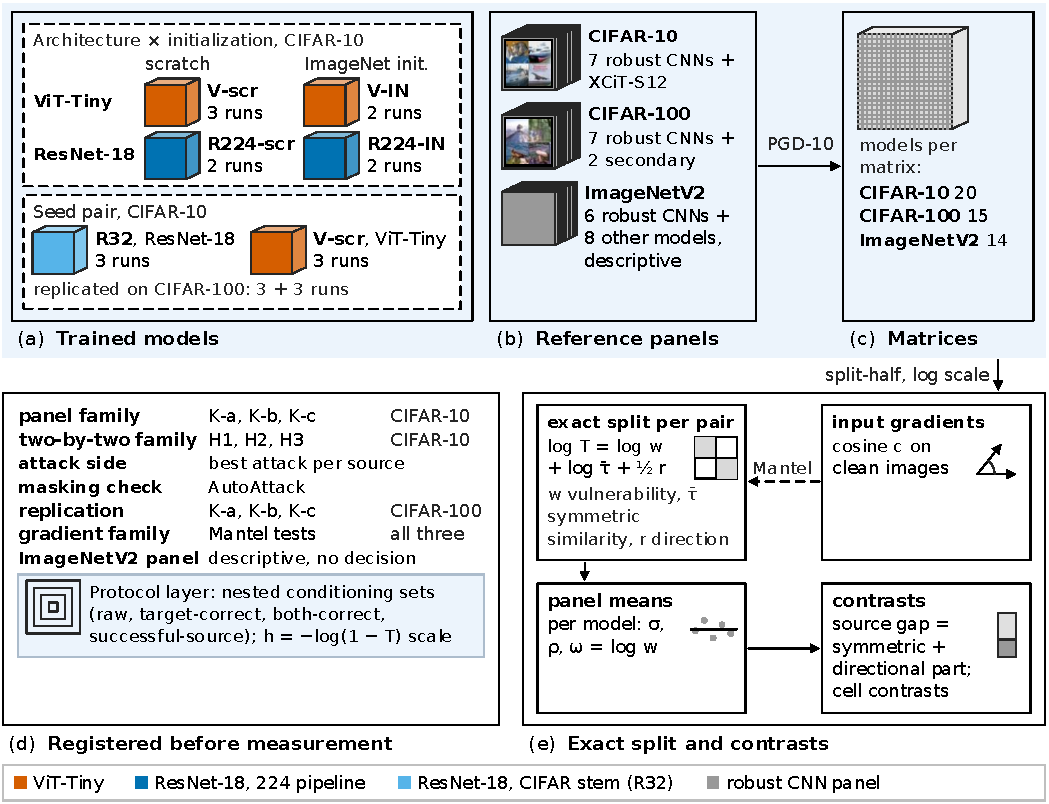
\includegraphics[width=\textwidth]{../figures/fig1_study_overview.pdf}
\caption{\textbf{Çalışmanın genel görünümü.} (a) Trained models, (b) Reference panels ve (c) Matrices panellerinde çift ve $2\times2$ tasarım, gürbüz CNN'lerden oluşan sabit panellere karşı PGD-10 saldırısıyla değerlendirilmektedir (panel üyeleri Şekil~\ref{fig:panel_members} içinde). (d) Registered before measurement paneli test ailelerini, (e) Exact split and contrasts paneli ise her matrisin log ölçeğinde bölünmüş yarı kestirimlerle ayrıştırılmasını vermektedir. Renkler ViT-Tiny'yi, iki ResNet-18 hattını ve paneli birbirinden ayırmaktadır.}
\label{fig:study_overview}
\end{figure*}

% ----------------------------------------------------------------------------
% 3.1 Tehdit modeli ve modeller
% ----------------------------------------------------------------------------
\subsection{Tehdit Modeli ve Modeller}
\label{subsec:setup}

% KAYNAK: ON_KAYIT Sec. 2-3 (eps, alpha, girdi hatti, timm adlari); EK Sec.
% 5.2 (ImageNetV2 eps 4/255, alpha 1/255); parametre sayilari eski metin
% 03:43 ve 03:47 (tasarim olgusu, sonuc degil).
% KAYNAK: raporlar/konsey_2026-10-29/_ek_flop_olcumu.json (param_M 5.53, on sinifli baslik; birlesik.md m10)
Bütün saldırılar hedefsizdir ve $\Linf$ normuyla, $\mathcal{B}_\eps(x) = \{x' : \|x' - x\|_\infty \leq \eps\}$ bölgesi içinde sınırlanmaktadır. Pertürbasyon bütçesi CIFAR-10 ve CIFAR-100~\cite{krizhevsky2009learning} için $\eps = 8/255$, ImageNetV2 için $\eps = 4/255$ olarak belirlenmiştir.

% KAYNAK: raporlar/hakem_konsey_2026-10-31/uygulama.md Sec. 9 (timm 1.0.27 vit_tiny_patch16_224, konteynerde okundu:
% patch_size 16, depth 12, embed_dim 192, num_heads 3, img_size 224); ON_KAYIT Sec. 3 (32->224 bilinear buyutme; degerler 32, 224).
Eğitilen modellerin tasarımdaki yeri Şekil~\ref{fig:study_overview}(a) içinde gösterilmiştir. Bu çalışmada R32 olarak anılan CIFAR ResNet-18~\cite{he2016deep}, $3\times3$ bir giriş katmanına ve 11{,}2M parametreye sahiptir ve $32\times32$ girdi almaktadır. ViT-Tiny (\texttt{timm}~\cite{rw2019timm}; 5{,}5M parametre, $16\times16$ yamalar, 3 başlı ve 192 genişlikli 12 blok) ile $7\times7$ giriş katmanlı \texttt{timm} \texttt{resnet18} modeli olan R224, 32 pikselden 224 piksele çift doğrusal olarak büyütülmüş girdileri okumaktadır. ImageNet ağırlıkları \texttt{deit\_tiny\_patch16\_224.fb\_in1k}~\cite{touvron2021training} ve \texttt{resnet18.a1\_in1k}~\cite{wightman2021resnet} kontrol noktalarından alınmıştır. CIFAR modelleri $[0,1]$ aralığındaki ham pikselleri okurken ImageNet ile başlatılan modeller ImageNet normalizasyonunu model içinde uygulamaktadır.

% ----------------------------------------------------------------------------
% 3.2 Saldirilar
% ----------------------------------------------------------------------------
\subsection{Saldırı Yöntemleri}
\label{subsec:attack_methods}

% KAYNAK: ON_KAYIT Sec. 5 B5 (MI-PGD mu 1.0, alpha eps/10; TGR alpha 2/255,
% mu 1.0, gamma 0.5; adim 10); eski metin 03:62-69 ve 03:171 (TGR uyarlamasi).
PGD~\cite{madry2018towards}, düzgün dağılımlı rastgele bir başlangıçtan çapraz entropi üzerinde $\alpha = 2/255$ (ImageNetV2'de $1/255$) boyunda on işaretli gradyan adımı atmakta ve her adımdan sonra $\mathcal{B}_\eps(x)$ üzerine izdüşüm almaktadır. Bu PGD-10 eğitimde, beyaz kutu değerlendirmede ve bütün transfer matrislerinde kullanılmıştır. AutoAttack~\cite{croce2020reliable}, APGD-CE, APGD-T, FAB-T ve Square saldırılarından oluşan standart topluluktur. Sonucun saldırıya bağlılığını yoklamak için iki kaynak saldırısı daha eklenmiştir. Bunlardan ilki MI-FGSM'i~\cite{dong2018boosting} izleyen momentumlu PGD-10'dur ($\mu = 1{,}0$, $\alpha = \eps/10$). İkincisi ise yalnız ViT kaynaklarında uygulanan ve momentumu $1{,}0$, adım boyu $\alpha = 2/255$, ölçek katsayısı $\gamma = 0{,}5$ olan TGR'dir~\cite{zhang2023tgr} (Bölüm~\ref{subsec:rw_transfer}). Bu çalışmadaki TGR dikkat, QKV ve MLP yollarına tek bir $\gamma$ uyguladığından ve her örnek ve kanal için jetonlar boyunca yalnız bir en büyük ve bir en küçük girdiyi sıfırladığından sonuçları yalnız bu uyarlama için geçerlidir.

Her kaynağın en iyi saldırısı, izin verilen saldırılar arasından örnekleri panele en iyi transfer olan saldırıdır. Seçim çift indisli görüntülerde yapılıp tek indisli görüntülerde puanlanmış, ardından roller değiştirilmiş ve kaynak açığı bu seçim altında yeniden hesaplanmıştır (Bölüm~\ref{subsec:decomposition_def}). Adım boyları saldırılar arasında farklıdır ve ayarlanmamıştır.

% ----------------------------------------------------------------------------
% 3.3 Egitim
% ----------------------------------------------------------------------------
\subsection{Çekişmeli Eğitim}
\label{subsec:training}

% KAYNAK: eski metin 03:78-100 (C1 tarifi, dogrulama bolmesi, tohumlar);
% CLAUDE.md (LR secimi). Tasarim sabitleri, sonuc degil.
Bütün modellerde $\tfrac12\mathcal{L}_{\mathrm{CE}}(f_\theta(x), y) + \tfrac12\mathcal{L}_{\mathrm{CE}}(f_\theta(x_{adv}), y)$ kaybı enküçültülmekte, $x_{adv}$ ise Rice vd.'nin~\cite{rice2020overfitting} referans gerçeklemesinde olduğu gibi model eğitim kipindeyken PGD-10 ile üretilmiştir. Kaybın yarısı temiz olduğundan ve eğitim temiz kontrol noktalarından başladığından bu karma kayıplı PGD çekişmeli ince ayar, Madry vd.'nin~\cite{madry2018towards} PGD çekişmeli eğitimiyle aynı yöntem değildir ve ürettiği gürbüz doğruluklar o yöntemin referans sonuçlarıyla karşılaştırılarak okunmamalıdır. Mimarinin savunmayla karışmaması için her hücrede tek bir tarif kullanılmıştır.

% KAYNAK: scripts/run_c1_pipeline.sh (temiz 200 epok, SGD lr 0.1, batch 128; AT 100 epok, lr 1e-3, ViT batch 64, sabir 20;
% tohumlar 1001-1003 ve 2001-2003); src/training/trainer.py (SGD weight_decay 5e-4, AdamW weight_decay 0.05);
% cli/train.py (--grad-clip 10); experiments/rev2/make_val_split.py (val-size 2000, split-seed 777); CLAUDE.md (min_delta 0.1).
R32 ve ViT-Tiny'nin temiz eğitiminde kosinüs tavlama~\cite{loshchilov2016sgdr} uygulanmış, CNN'de SGD (ağırlık sönümü $5\times10^{-4}$), ViT'te AdamW~\cite{loshchilov2017decoupled} (ağırlık sönümü 0{,}05) kullanılmıştır. Ardından gelen çekişmeli ince ayar da kosinüs çizelgesiyle yürütülmüş, her koşunun epok sayısı, öğrenme oranı, parti boyu ve tohumları Şekil~\ref{fig:design_recipe} içinde verilmiştir. İnce ayarda gradyanlar $L_2$ normu 10'da kırpılmış, sonlu olmayan partiler atlanmış ve veri artırma 4 piksel dolgulu rastgele kırpma ile yatay çevirmeyle yapılmıştır. Seçim ve erken durdurma (sabır 20, eşik 0{,}1 puan), sabit 2.000 görüntülük bir doğrulama bölmesindeki PGD-10 doğruluğuna dayanmaktadır. Bu bölme tohum 777 ile bir kez çekilmiş ve her modelin iki eğitim aşamasından da çıkarılmıştır. Tohumlar indekse göre eşlenmiş, tablolar ise koşular üzerinden ortalama ve standart sapma vermektedir.

% 2026-10-04 (koordinator karari): onceki cift karantinadadir; hicbir sayisi metne girmez.
Temiz ön eğitimin zaten gördüğü bir doğrulama bölmesiyle seçilmiş daha eski bir kontrol noktası çifti de aynı mutlak sıralamayı vermiştir. Ancak bu çift sızıntısız protokolden önceye ait olduğundan hiçbir sayısı bu makaleye girmemektedir.

% ----------------------------------------------------------------------------
% 3.4 Mimari x baslatma tasarimi
% ----------------------------------------------------------------------------
\subsection{Mimari \texorpdfstring{$\times$}{x} Başlatma Tasarımı}
\label{subsec:design}

% KAYNAK: ON_KAYIT Sec. 3 (hucreler, tarif, normalizasyon demeti), Sec. 4
% (denetimler); FOY:M9:1443 (hucre tanimlari).
Sıfırdan eğitilmiş bir ViT-Tiny, R32'den mimari, girdi hattı ve belki de eğitimin yeterliliği bakımından ayrılmaktadır. ViT'lerin çekişmeli eğitiminin ön eğitime bağlı olduğu da bilinmektedir~\cite{mo2022adversarial}. Şekil~\ref{fig:design_recipe} ile verilen tasarım bu etkenleri birbirinden ayırmak için kurulmuştur. \cellname{R224-scr}, ViT-Tiny koşularının (\cellname{V-scr}) girdi hattını ve temiz aşama komutunu paylaşmaktadır. Böylece sıfırdan satırındaki iki hücre mimari paketinde, \cellname{V-scr} için ayrıca eğitim kampanyasında ve çekişmeli epok tavanında ayrışmakta, ImageNet satırı ise iki mimariyi de ImageNet ağırlıklarından başlatmaktadır. Başlatma etkeni ağırlıkları, daha kısa bir AdamW temiz aşamasını ve model içi normalizasyonu bir demet hâlinde taşımaktadır. Bu demet iki mimari için aynı olduğundan etkileşim karşıtlığından ancak etkisi mimariye bağlı değilse düşmekte, normalizasyonun ayrı etkisi ise tanımlanamamaktadır.

% Sekil 2: paper/figures/fig2_design_recipe.pdf (visio-cizici Uslup 8; eski Tablo 1 tab:design yerine; sayilar
% results/q1/konsey_b3_tarif.json ve foy M13, kanit fig2_design_recipe.kanit.json). Altyazida sayi yok.
\begin{figure}[!t]
\centering
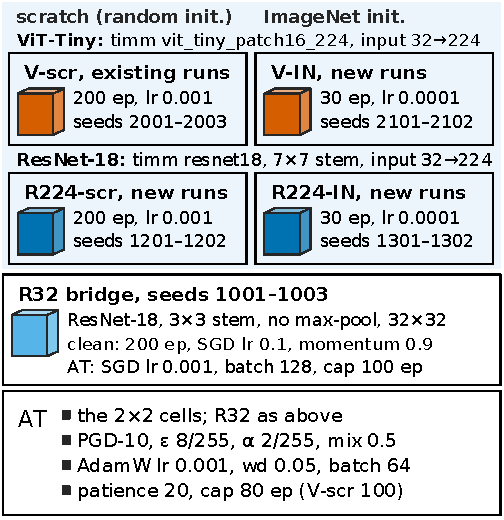
\includegraphics[width=\columnwidth]{../figures/fig2_design_recipe.pdf}
\caption{\textbf{Mimari $\times$ başlatma tasarımı.} CIFAR-10'da ViT-Tiny ve ResNet-18 satır şeritleri, scratch (random init.) ve ImageNet init. sütun şeritleriyle kesişmektedir. Her hücre temiz aşamasını (epok, öğrenme oranı) ve tohumlarını vermekte, var olan koşular özgün çiftten, yenileri ise B3 bloğundan gelmektedir. R32 köprüsü kendi tarifini korumakta, AT şeridi de dört hücrenin çekişmeli tarifini göstermektedir.}
\label{fig:design_recipe}
\end{figure}

% KAYNAK: ON_KAYIT Sec. 4 (denetim esigi 5 puan, cokus esigi 15 yuzde, kirpilma, dislama).
ImageNet ile başlatılan her koşunun, ilk temiz epoğundan sonra, kendi mimarisindeki rastgele başlatılmış koşuların ilk epok doğrulama doğruluğu ortalamasını 5 puan aşması gerekmiştir. Bu koşul, yüklemenin ve normalizasyonun bir denetimi olarak konmuştur. Beşinci çekişmeli epokta doğrulama PGD doğruluğunun \%15'in altında kalması durumunda ImageNet satırının öğrenme oranının düşürülmesi öngörülmüştür. Tavana beş epoktan daha yakın bir noktada seçilen koşu kesilmiş olabileceği gerekçesiyle işaretlenmekte, hiçbir koşu sonuçlarına bakılarak dışlanmamaktadır. Kayıtlı karşıtlıklar $\sigma$ ve $\rho$'nun hücre ortalamalarını kullanmaktadır (Denklem~\eqref{eq:panel_def}):
\begin{align*}
\Asig{scr} &= \sigma(\cellname{V-scr}) - \sigma(\cellname{R224-scr}),\\
\Isig &= [\sigma(\cellname{V-IN}) - \sigma(\cellname{V-scr})]\\
&\quad - [\sigma(\cellname{R224-IN}) - \sigma(\cellname{R224-scr})],\\
\Arho &= \tfrac12\{[\rho(\cellname{V-scr}) - \rho(\cellname{R224-scr})]\\
&\quad + [\rho(\cellname{V-IN}) - \rho(\cellname{R224-IN})]\}.
\end{align*}

% ----------------------------------------------------------------------------
% 3.5 Ayrisim
% ----------------------------------------------------------------------------
\subsection{Kırılganlık, Benzerlik ve Yön}
\label{subsec:decomposition_def}

% KAYNAK: ON_KAYIT Sec. 2 (tanimlar, bolunmus yari, logit ve oran olcekleri,
% panel uyesinin kendi degeri); 01_oneri_P3_kuram_olcum.md satir 15-27
% (Onerme 1); brif Sec. 3.1 gosterim.
% KAYNAK: eski metin 03:109-116 (T_ij tanimi; 2026-10-31 subsec:metrics'ten tasindi).
Gürbüz doğruluk temizde yanlış sınıflandırılan görüntüleri gürbüz olmayan saydığından temiz doğruluk ile koşullu sağkalımın çarpımına birebir ayrışmaktadır. Koşullu sağkalımın tümleyeni, $j$ modelinin beyaz kutu koşullu yanıltma oranı $w_j$'dir. Kaynak $i$'den hedef $j$'ye transferde \emph{hedef doğru} oranı, $j$'nin temizde doğru sınıflandırdığı ve $i$ üzerinde üretilen örnekte yanlış sınıflandırdığı görüntülerin kesridir:
\begin{equation}
    T_{ij} = \frac{\sum_{x} \mathbf{1}[f_j(x) = y]\,\mathbf{1}[f_j(x_{adv}^{(i)}) \neq y]}{\sum_{x} \mathbf{1}[f_j(x) = y]}.
\end{equation}
Bu tanımla $w_j = T_{jj}$ olur.

Hedef doğru oranları $T_{ij}$, $T_{ji}$ ve beyaz kutu oranları $w_i$, $w_j$ olan iki model için
\begin{align}
\log\simt_{ij} &= \tfrac12\left[\log(T_{ij}T_{ji}) - \log(w_i w_j)\right], \label{eq:tau_def}\\
r_{ij} &= \log(T_{ij}/T_{ji}) - \log(w_j/w_i) \label{eq:r_def}
\end{align}
tanımlandığında
\begin{equation}
\log T_{ij} = \log w_j + \log\simt_{ij} + \tfrac12 r_{ij}
\label{eq:decomp}
\end{equation}
eşitliği birebir sağlanır. Burada benzerlik $\simt_{ij} = \simt_{ji}$ iki yön tarafından paylaşılmakta, yönlü artık $r_{ij} = -r_{ji}$ ise kırılganlık oranı çıkarıldıktan sonra kalan log asimetrisini vermektedir. Denklem~\eqref{eq:decomp} bir muhasebe özdeşliğidir. Bu özdeşliğin içeriği terimlerin ölçülen büyüklüklerinde ve bu büyüklüklerin tasarıma verdiği yanıtta yatmaktadır. $r$ olmadan yazılan $T_{ij} = w_j\simt_{ij}$, sütun etkisi ölçülmüş bir değere sabitlenmiş hâliyle Caussinus'un~\cite{caussinus1965contribution} yarı simetri modelidir (Bölüm~\ref{subsec:rw_decomposition}). Bu biçimiyle Demontis vd.'nin~\cite{demontis2019adversarial} üç etkeninden ikisine, hedef kırılganlığına ve gradyan hizalanmasına yakın durmaktadır. Üçüncü etken olan vekil modelin karmaşıklığına ayrı bir terim ayrılmamış, bu etken Önerme~\ref{prop:identifiability}(d)'nin anlattığı biçimde öteki terimlere katılmıştır (Şekil~\ref{fig:decomposition_schematic}).

% Sekil 3: paper/figures/fig3_decomposition_schematic.pdf (visio-cizici Uslup 8; kanit fig3_decomposition_schematic.kanit.json); manifest gosterim.altyazi_notu: T(i, j) = T_ij.
\begin{figure}[!t]
\centering
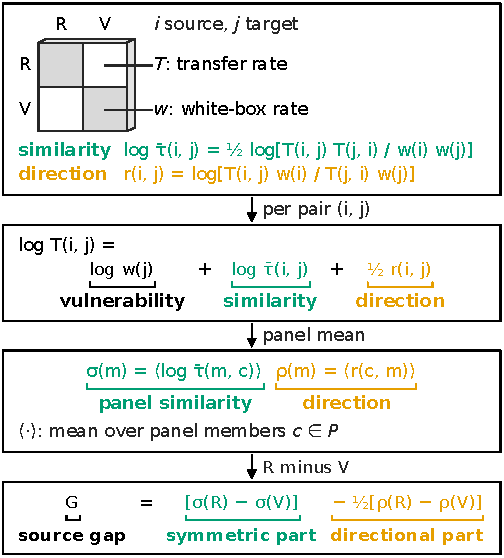
\includegraphics[width=\columnwidth]{../figures/fig3_decomposition_schematic.pdf}
\caption{\textbf{Çalışma boyunca kullanılan ayrışım.} Yukarıdan aşağıya per pair $(i, j)$, panel mean ve R minus V köşeli okları üç adımı işaretlemektedir. Log hedef doğru oranı kırılganlığa, benzerliğe ve yönlü artığın yarısına birebir ayrışmakta, panel ortalamaları $\sigma$ ile $\rho$'yu vermekte, kaynak açığı $G$ ise simetrik ve yönlü parçalara bölünmektedir. Şekildeki $T(i, j)$ gösterimi $T_{ij}$ anlamındadır; $w$, $\simt$ ve $r$ için de aynı gösterim kullanılmıştır.}
\label{fig:decomposition_schematic}
\end{figure}

% KAYNAK: ON_KAYIT Sec. 2 (oranlar yuzde olarak; logit tanimi x/100, dolayisiyla sabit log 100; deger 100).
Model düzeyindeki nicelikler dış modellerden oluşan sabit bir $P$ paneli üzerinden ortalanmaktadır:
\begin{equation}
\begin{gathered}
\sigma_m = \frac{1}{|P|}\sum_{c\in P}\log\simt_{mc}, \qquad \rho_m = \frac{1}{|P|}\sum_{c\in P} r_{cm},\\
\omega_m = \log w_m.
\end{gathered}
\label{eq:panel_def}
\end{equation}
Yüksek bir $\sigma_m$, $m$'nin çekişmeli yönleri panelle paylaştığını gösterir. Pozitif bir $\rho_m$ ise $m$'nin, kırılganlığın açıklayabildiğinin ötesinde, panelden gönderdiğinden fazlasını aldığı, yani yönlü olarak zayıf bir kaynak olduğu anlamına gelir. Oranlar logaritmaya yüzde olarak girdiğinden $\omega$ ve aşağıdaki $L_k$, her karşıtlıktan düşen toplamsal bir $\log 100$ sabiti taşımakta, $\sigma_m$ ise ayrıca $w$'nin yakalamadığı her model ana etkisinin yarısını da üstlenmektedir. $R$ ve $V$ modelleri için panel kaynak açığı
\begin{equation*}
G = \frac{1}{|P|}\sum_{c\in P}\left[\log T_{Rc} - \log T_{Vc}\right] = (\sigma_R - \sigma_V) - \tfrac12(\rho_R - \rho_V)
\end{equation*}
olarak tanımlanmakta ve $V$'nin üçüncü modellere karşı $R$'den ne kadar zayıf bir kaynak olduğunu ölçmektedir. Bu açığın simetrik payı $q = (\sigma_R - \sigma_V)/G$'dir. Tohum çifti $s$ için $q_s$, çiftler üzerinden ortalama için $q$ yazılmakta, panelin kendi kırılganlıkları bu paydan düşmektedir. Saf bir kaynak etkisi, K-a'nın sıfır değeri olan $q = 1/2$'yi verir ve daha büyük bir $q$, kaynak etkisinin ötesindeki farklılığı ölçer. Kaynak saldırısı $k$ için $L_k(m) = |P|^{-1}\sum_{c\in P}\log T_k(m\to c)$, $m$ kaynağının panel ortalamalı log transferidir ve böylece $G = L_{\mathrm{PGD}}(R) - L_{\mathrm{PGD}}(V)$ olur. $\Gk{k}$ aynı farkın R32 ve ViT-Tiny koşuları için $k$ saldırısı altındaki değeridir. Korunan oran $\Gk{best}/\Gk{PGD}$ ise açığın her kaynağın en iyi saldırısı altında korunup korunmadığını sorar (Bölüm~\ref{subsec:attack_methods}). Aile içi benzerlik $\Dseed$, ViT tohum çiftleri üzerinden ortalama $\log\simt$ değerinden bu tohumların $\sigma$ ortalamasının çıkarılmasıyla elde edilir.

\begin{proposition}[Tanımlanabilirlik]
\label{prop:identifiability}
Aşağıda $i \neq j$ için $\ell_{ij} = \log T_{ij}$ yazılmaktadır. (a) İki modelde $\ell$'nin antisimetrik kısmı tek bir sayıdan, $\ell_{12} - \ell_{21}$ farkından ibarettir. Simetrik $s$ ile kurulan $\ell_{ij} = \mu + \alpha_i + \beta_j + s_{ij}$ toplamsal uydurması yalnız $(\alpha_1 - \alpha_2) - (\beta_1 - \beta_2)$ farkını tanımlar, bu farkın kaynak ile hedef arasındaki bölüşümünü tanımlamaz. (b) $\ell_{ij}$ bir $\gamma\,\mathbf{1}[i,j \in C]$ aile terimi içeriyorsa ve tasarımda $C$'ye ait olmayan tek bir $V$ modeli varsa toplamsal uydurma bu terimi $V$'nin kaynak ve hedef etkilerine eşit $-\gamma$ ağırlığıyla katar ve asimetriyi değiştirmez. (c) $\ell_{ij}$ içindeki her simetrik terim, aile terimi de dâhil, $r_{ij}$'den düşer ve $\log\simt_{ij}$'ye bütünüyle girer, sabit bir panel üzerinde de $\sigma_m$'yi değiştirip $\rho_m$'yi değiştirmez. (d) $\ell_{ij}$ içindeki bir $\alpha_i$ kaynak ana etkisi $r_{ij}$'ye $\alpha_i - \alpha_j$ potansiyel farkı olarak, $\log\simt_{ij}$'ye ise $\tfrac12(\alpha_i+\alpha_j)$ olarak girer. $R$ ile $V$ arasında simetrik bir fark yoksa bu etki $q = 1/2$ verir.
\end{proposition}

(a) şıkkı, $K$ model için $K-1$ potansiyel ve $(K-1)(K-2)/2$ dolaşım serbestlik derecesi veren Hodge ayrışımının~\cite{jiang2011statistical} serbestlik derecesi sayımından gelmektedir. (b) şıkkı $i\neq j$ için $\mathbf{1}[i,j\in C] = 1 - \mathbf{1}[i=V] - \mathbf{1}[j=V]$ eşitliğinden, (c) ve (d) şıkları ise Denklem~\eqref{eq:tau_def} ve~\eqref{eq:r_def} içinde yerine koymadan çıkmaktadır. Dolayısıyla tek bir ViT bulunan bir tasarımda ViT'in toplamsal bir kaynak etkisi CNN'lerden farklılığından ayırt edilemez ve ayrışım bu farklılığı $\sigma$'ya yüklemektedir.

Kestirimler bölünmüş yarı düzeniyle yapılmaktadır (Şekil~\ref{fig:study_overview}(e)). $w$ çift indisli test görüntülerinden, $T$ tek indisli görüntülerden alınmış, ardından roller değiştirilip iki yarının ortalaması hesaplanmış ve böylece bir köşegen hücresi ile bir köşegen dışı hücre hiçbir zaman aynı görüntüleri paylaşmaz. $\omega$ ise tam örneklemden hesaplanan $w$'yi kullanmaktadır. Bir panel üyesinin kendi $\sigma$ ve $\rho$ değerleri o üye dışarıda bırakılarak hesaplanmıştır. Doğal logaritma birincil ölçektir. Duyarlılık analizi olarak logit ölçeği $\log x$ yerine $\log[x/(1-x)]$ kullanmakta, oran ölçeği ise oranların kendisiyle çalışmaktadır.

% ----------------------------------------------------------------------------
% 3.6 Paneller
% ----------------------------------------------------------------------------
\subsection{Referans Panelleri}
\label{subsec:panels}

% KAYNAK: ON_KAYIT Sec. 2 ve Dondurma eki (c) (P yedi uye, XCiT ikincil,
% en az bes uye); EK Sec. 4.1 (P9), Sec. 5.1-5.5 (ImageNetV2, P8, ciftler,
% on isleme denetimi). FOY:M9.4:1569 (CIFAR-10 K = 20); FOY:M10.1:1820
% (ImageNetV2 n = 2000), 1826 (CIFAR-100 15 model), 1827 (ImageNetV2 14 model).
% 2026-10-31 visio-cizici Faz C: uye adlari (RobustBench kimlikleri) Sekil 4'e (fig:panel_members) tasindi;
% atiflar metinde kaldi (altyazi 60 sozcuk siniri). Ortak hat kurallari, gosterim, Liu ve Mo metinde.
Panel üyeleri RobustBench'ten~\cite{croce2021robustbench} alınmış, her panel transfer hücreleri hesaplanmadan önce dondurulmuş ve bütün üyeler tanımlayıcılarıyla Şekil~\ref{fig:panel_members} içinde listelenmiştir. CIFAR panellerinin üyeleri~\cite{wong2020fast, engstrom2019robustness, carmon2019unlabeled, gowal2020uncovering, sehwag2022robust, addepalli2022efficient, rade2022reducing, rice2020overfitting, pang2022robustness, wang2023better, jia2022lasat, debenedetti2023light, hendrycks2019using} çalışmalarından alınmıştır. CIFAR-10'daki birincil $P$ paneli, ImageNet ön eğitimi olmadan eğitilmiş ve ResNet ailesinden gelen yedi $\Linf$-gürbüz CNN'den oluşmakta, bunların dördü (PreAct) ResNet-18 türevidir. ImageNet ile ön eğitilmiş XCiT-S12 ise ikincil paneli oluşturmaktadır (Şekil~\ref{fig:study_overview}(b)). Çift ve tasarım hücreleriyle birlikte CIFAR-10 matrisi 20 model içermektedir (Şekil~\ref{fig:study_overview}(c)).

% FOY:M10.1:1826 (CIFAR-100 matrisi 15 model)
CIFAR-100 paneli, RobustBench'in elverdiği ölçüde $P$'ye yakın tutulmuş ve yedi CNN'den kurulmuştur. ImageNet ile ön eğitilmiş XCiT-S12 ve Hendrycks vd.'nin modeli ikincil paneli oluşturmaktadır. Bu veri kümesindeki çift, her biri üç tohumlu CIFAR-100 ResNet-18 ve ViT-Tiny modelleridir ve eğitildikleri dönemde geçerli olan, CIFAR-10 kuralından farklı tek bölmeli kurala göre seçilmiştir. Bu veri kümesindeki matris 15 model içermektedir.

% FOY:M10.1:1820,1827 (ImageNetV2 n = 2000; 14 model)
% KAYNAK: EK Sec. 5.2-5.5 (ortak hat Resize 256 ve CenterCrop 224; 1000 sinif logit; kendi hatla temiz dogruluk
% en az 25 yuzde ve RobustBench degerinin 0.6 kati; degerler 256, 224, 1000, 25, 0.6).
ImageNet paneli altı CNN'den oluşmaktadır~\cite{salman2020adversarially, engstrom2019robustness, chen2024data, peng2023robust}. Temiz eğitilmiş modellerden ortak bir tarifle çekişmeli olarak eğitilmiş ve hepsi evrişimli giriş katmanı taşıyan iki CNN-dönüştürücü çifti, yani ConvNeXt-T ile ViT-S ve ConvNeXt-B ile ViT-B~\cite{singh2023revisiting}, ImageNet ile başlatılmış satırı oluşturmaktadır. $k$ çifti için dönüştürücü eksi CNN farkları $\sigma$, $\rho$ ve $\omega$'da sırasıyla $\Ak{\sigma}{k}$, $\Ak{\rho}{k}$ ve $\Ak{\omega}{k}$ ile, $\Ak{\sigma}{k}$'nin bu iki çift üzerinden ortalaması ise $\AbarIN$ ile gösterilmektedir. Liu vd.'nin~\cite{liu2023comprehensive} ConvNeXt-B ve Swin-B modelleri sıfırdan satırını vermektedir. Ancak ortak yapılandırmalarında bir ön eğitim bayrağı bulunmadığından bu dayanak dolaylıdır. Bu çiftin karşıtlığı, CIFAR-10 karşıtlığı $\Asig{scr}$ ile karışmaması için $\Asig{scr,Liu}$ ile yazılmaktadır. Mo vd.'nin ViT-B modeli~\cite{mo2022adversarial} eşi olmadan, XCiT-S12 ise ikincil üye olarak matrise girmekte ve toplam 14 model, ImageNetV2 MatchedFrequency kümesinin~\cite{recht2019imagenet} 2.000 görüntüsü üzerinde değerlendirilmektedir. Bu görüntüler her sınıfın sözlük sırasındaki ilk iki dosyasından oluşmaktadır. Bütün modellere tek bir ön işleme hattı (256 piksele bikübik yeniden boyutlandırma, 224 piksele merkez kırpma) uygulandığından bir kaynağın çekişmeli tensörü her hedefe aynı piksel uzayında ulaşmaktadır. Normalizasyon her RobustBench modelinin uyguladığı biçimde bırakılmış, puanlamada 1.000 logitin tamamı kullanılmıştır. Her modelin kendi hattındaki temiz doğruluğunun \%25'e ve RobustBench değerinin 0{,}6 katına ulaşması, ortak hattaki doğruluktan da en çok 5 puan ayrılması gerekmiştir. Bu panel betimseldir ve $2\times2$ tasarımı yinelememektedir. Panelde başlatma aynı veri kümesinde yapılmış temiz ön eğitim anlamına gelmekte, mimariler de farklı bulunmaktadır.

% Sekil 4: paper/figures/fig4_panel_members.pdf (visio-cizici Uslup 8; yeni sekil Y2; kaynak hucre_tablosu.json, _b9, _b8 birincil/ikincil panel alanlari).
\begin{figure}[!t]
\centering
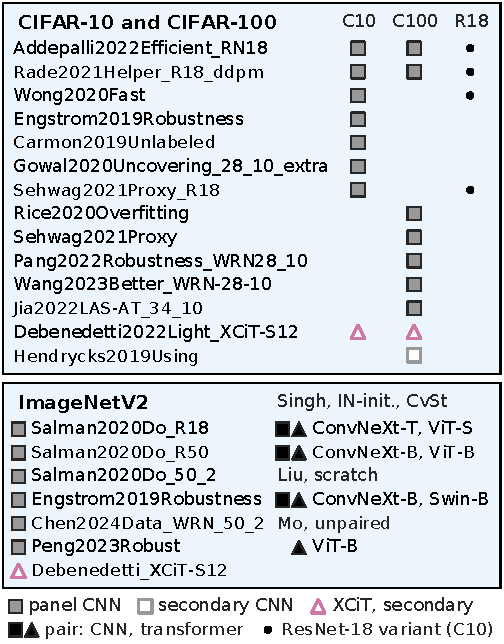
\includegraphics[width=\columnwidth]{../figures/fig4_panel_members.pdf}
\caption{\textbf{Referans paneli üyeleri.} CIFAR-10 and CIFAR-100 başlıklı üst blok, her RobustBench tanımlayıcısının rolünü C10 ve C100 sütunlarında vermekte, ResNet-18 türevlerini de R18 sütununda işaretlemektedir. ImageNetV2 başlıklı alt blok solda CNN panelini ve ikincil XCiT-S12'yi, sağda ise dönüştürücü çiftlerini ve Mo vd.'nin eşi olmayan ViT-B modelini listelemektedir.}
\label{fig:panel_members}
\end{figure}

% ----------------------------------------------------------------------------
% 3.7 Kosullama protokolleri (2026-10-31 hakem konseyi B16: ayrisim ve panellerin ardina alindi;
% T_ij tanimi ayrisim alt bolumune tasindi, boylece tanimlanabilirlik Onerme 1, h olcegi Onerme 2)
% ----------------------------------------------------------------------------
\subsection{Koşullama Protokolleri}
\label{subsec:metrics}

% KAYNAK: scripts/q1_e2_conditional.py (ornek bazli bootstrap, --n-boot 10000; tam test kumesi).
Köşegeni de aynı biçimde koşullandığı için ayrışımda baştan sona hedef doğru oranı kullanılmaktadır. Doğru sınıflandırılan görüntülerle koşullama yerleşik bir uygulamadır (Bölüm~\ref{subsec:rw_protocols}). Ne var ki koşullama kümesi bir protokol seçimidir ve protokol katmanı (Bölüm~\ref{subsec:transfer}) aynı örnek bazındaki kayıtlar üzerinde üç alternatifi puanlamaktadır. Bunlar koşulsuz oran, \emph{her ikisi doğru} oranı~\cite{mahmood2021robustness, ravikumar2023trend} ve Ravikumar vd.'nin~\cite{ravikumar2023trend} \emph{başarılı kaynak} oranıdır ve bunların maskeleri o bölümdeki Şekil~\ref{fig:protocol_sets} üst kartında gösterilmiştir. Sonuncusu, beyaz kutu başarısının temizde doğru sınıflandıran bir kaynağı varsaydığı sıkı okumayla uygulanmakta, bu koşulu aramayan gevşek okuma ise yalnız duyarlılık analizi olarak kullanılmaktadır. Koşulsuz ve her ikisi doğru maskeleri bir çiftin iki yönünde aynı örnekleri kullanırken hedef doğru ve başarılı kaynak maskelerinde iki yönün örnekleri farklıdır. Oranlar örnek bazındaki sonuçları kaydedilmiş tam test kümelerinde hesaplanmakta, sabit kontrol noktalarının aralıkları ise görüntüler üzerinde 10.000 yeniden örneklemeli yüzdelik bootstrap ile elde edilmektedir.

Hedefin temiz hatası $e$, bir yönün koşulsuz ve hedef doğru oranları $r_{\text{ham}}$ ve $r_{\text{koş}}$ ($r_{\text{koş}} = T_{ij}$), hedefin temiz girdide yanlış sınıflandırdığı bir örneğin kaynakta üretilmiş girdide de yanlış sınıflandırılma olasılığı ise $p$ ile gösterilsin. Toplam olasılık yasasına göre
\begin{equation}
r_{\text{ham}} = e\,p + r_{\text{koş}}\,(1 - e)
\label{eq:general_identity}
\end{equation}
olur ve $p=1$ olduğunda
\begin{equation}
r_{\text{ham}} - r_{\text{koş}} = e\,(1 - r_{\text{koş}})
\label{eq:raw_identity}
\end{equation}
elde edilir. Tek bir model üzerinde $p=1$ tanım gereği sağlanırken transferde sabit bir pertürbasyon yanlış sınıflandırılmış bir örneği doğru sınıfa geri taşıyabileceğinden $p$'nin ölçülmesi gerekir. Denklem~\eqref{eq:general_identity}, tek görgül içeriği $p$ olan bir muhasebe özdeşliğidir. Buna karşılık $p<1$ olduğunda Denklem~\eqref{eq:raw_identity} sapmayı $e\,(1-p)$ kadar abartmaktadır. $h = -\log(1-T)$ ölçeğinde ise aynı özdeşlik, protokolün hangi sonuçları değiştirebileceğini de göstermektedir.

\begin{proposition}[$h$ ölçeğinde protokol ayar dönüşümü]
\label{prop:hscale}
Her $i \to j$ yönü için $g_{ij} = -\log\bigl(1 + e_j(1-p_{ij})/[(1-e_j)(1-T_{ij})]\bigr)$ olmak üzere $h^{\text{ham}}_{ij} - h^{\text{koş}}_{ij} = -\log(1 - e_j) + g_{ij}$ eşitliği sağlanır ve $g_{ij}$, $p_{ij} = 1$ olduğunda sıfırlanır. Dolayısıyla $h$ matrisinin toplamsal bir ayrışımındaki kaynak etkileri, ikili simetrik terimler ve dolaşım, $g$ dışında ham ve hedef doğru protokollerinde aynıdır. Yalnız hedef etkileri bilinen $-\log(1-e_j)$ miktarı kadar kaymaktadır.
\end{proposition}

Bu sonuç, Denklem~\eqref{eq:general_identity} $1 - r_{\text{ham}} = (1-e)(1-r_{\text{koş}}) + e(1-p)$ biçiminde yeniden düzenlenerek elde edilmektedir. Maskesi kaynağın temiz doğruluğuna bağlı olduğundan her ikisi doğru protokolü böyle bir ayar dönüşümü oluşturmamaktadır.

% ----------------------------------------------------------------------------
% 3.8 Girdi gradyani hizalanmasi
% ----------------------------------------------------------------------------
\subsection{Girdi Gradyanı Hizalanması}
\label{subsec:gradcos_def}

% KAYNAK: EK Sec. 6.1-6.3 (tanim, ham ve ana etki artikli Spearman,
% permutasyon 9999, tohum 20261030, karar kurali).
Simetrik terimin transfer ve saldırı olmadan ölçülebilen bir şeyi yansıtıp yansıtmadığı, her model çiftinde girdi gradyanlarının temiz görüntülerdeki ortalama kosinüsüyle yoklanmıştır:
\begin{equation}
c_{ij} = \frac{1}{n}\sum_{x} \cos\left(\nabla_x \mathcal{L}_i(x,y),\, \nabla_x \mathcal{L}_j(x,y)\right).
\label{eq:cij}
\end{equation}
Burada $\mathcal{L}_m$, $m$ modelinin çapraz entropisidir. Gradyanlar model içindeki normalizasyondan geçilerek $[0,1]$ piksel uzayında alınmış, modeller değerlendirme kipinde tutulmuş ve ilgili transfer matrisinin görüntüleri kullanılmıştır. Bu nicelik Zhang vd.'nin~\cite{zhang2024why} gradyan benzerliğinin görüntü ortalamasıdır, hizalanma ise Demontis vd.'nin~\cite{demontis2019adversarial} simetrik etkenine karşılık gelmektedir.

% FOY:M10.5:1970 (9999 permutasyon, p tabani 1e-4)
Ham istatistik, sırasız çiftler üzerinde $c_{ij}$ ile $\log\simt_{ij}$ arasındaki Spearman korelasyonu $\rS$'dir. Artık istatistiği ise her matrise kurulan $X_{ij} = \mu + a_i + a_j + e_{ij}$ en küçük kareler uydurmasının artıklarını ilişkilendirmektedir. Bu uydurma, gürbüzlük, gradyan normu ya da temiz doğruluk gibi bir çiftin iki üyesine de eklenen her model düzeyi özelliği ortadan kaldırmakta ve kısmi Mantel testinin~\cite{smouse1986multiple} mantığını bütün model ana etkilerini bir kerede çıkararak izlemektedir. Anlamlılık Mantel testinden~\cite{mantel1967detection} elde edilmektedir. Bu testte $\log\simt$ sabit tutulurken model etiketleri $c$'nin satır ve sütunları üzerinde birlikte 9.999 kez permüte edilmiş ve alt sınırı $10^{-4}$ olan tek yönlü bir $p$ değeri hesaplanmıştır. Toplamsal uydurma çarpımsal ya da etkileşimli model etkilerini ve CNN ile dönüştürücü ailelerinin blok yapısını yerinde bırakmaktadır.

% ----------------------------------------------------------------------------
% 3.9 Istatistiksel cikarim ve kayitli testler
% ----------------------------------------------------------------------------
\subsection{İstatistiksel Çıkarım}
\label{subsec:statistics}

% KAYNAK: ON_KAYIT Sec. 2, 5, 6 (cikarim birimi, delta, karar ilkesi, Holm,
% sonuc haritasi); EK Sec. 2, 4.2, 5.6, 6.3. delta = 0.10 ve 0.06 tasarim
% sabitidir. Dayanaktaki RMS degerleri (havuz r, 21 cift; yalniz CNN
% ciftleri) foyde yok, sayisiz yazildi.
Çıkarım birimi eğitim koşusu, görüntüler ise bütün modellerin paylaştığı yinelenen ölçümlerdir. Bu nedenle koşular üzerinden kurulan aralıklar sabit test görüntülerine ve panel üyelerine koşulludur ve görüntü örneklemesi yalnız görüntüleri yeniden örnekleyen bootstrap analizlerine girmektedir. Tasarımın $2\times2$ karşıtlıkları koşu düzeyindeki hücre ortalamalarını ve 5 serbestlik dereceli, birleştirilmiş varyanslı bir $t$ aralığını kullanmaktadır. Testler Şekil~\ref{fig:study_overview}(d) içindeki kayıtlı aileleri oluşturmakta ve her aile içinde $\alpha = 0{,}05$ düzeyinde Holm düzeltmesi uygulanmaktadır (Şekil~\ref{fig:registry_map}). Eşdeğerlik, $\delta = 0{,}10$ log birimlik marjla iki tek yönlü testle (TOST) sınanmaktadır. Bu marj bir oranda kabaca yüzde onluk göreli değişime karşılık gelmektedir. Eşdeğerlik testi log nicelikleri için kaydedildiğinden logit ve oran ölçeklerinde aynı banda karşı yapılan karşılaştırmalar betimseldir. Marj, ön kayıttan önce görülen çekişmeli eğitilmiş modeller arasındaki yönlü artığın karesel ortalama karekökünden (RMS) alınmıştır. Bu küme ViT'i de içerdiğinden marj gevşektir ve her eşdeğerlik, yalnız CNN çiftlerinden gelen değer olan $\delta = 0{,}06$ ile yinelenmektedir. $\sigma$ karşıtlıkları (H1, H2, K-c) için aynı marj, ayrı bir görgül dayanağı olmayan bir uzlaşımdır.

% KAYNAK: ON_KAYIT Sec. 6 satir 100 (O1 bolgesi ve onceden yazilmis manseti).
% KAYNAK: results/q1/konsey_kayit_kurallari.json (K-a payda kurali, B5 kurallari, H2 logit kosulu).
% FOY:M13:2528,2535,2547
Destek Holm düzeltmeli $p < 0{,}05$ değerinden okunmaktadır. Çürütme ile H1 ve H2'nin eşdeğerlik kolları ham aralıklardan, K-b ve H3 için eşdeğerlik desteği ise önce çürütme denetlenmek koşuluyla Holm düzeltmeli TOST $p$ değerinden okunmaktadır. Böylece aralığı $\pm\delta$ içinde kalan anlamlı bir etki ihmal edilebilir sayılmaktadır. Herhangi bir tohum çiftinde $G_s$ açığı $\delta$ değerini aşmıyorsa K-a kararsız sayılmaktadır. Korunan oran $\Gk{best}/\Gk{PGD}$ ise $\Gk{PGD} \leq \delta$ olduğunda kararsız sayılmakta, \%90 aralığının alt sınırı en az $0{,}5$ olduğunda desteklenmekte, üst sınırı $0{,}5$ değerinin altında kaldığında ise çürütülmektedir. H2'nin desteklenmesi için logit ölçeğindeki kestirimin de pozitif olması gerekmektedir. Hesaplanamayan bir test $p = 1$ sayılmakta, öngörülen büyüklükler ise ölçüt yapılmadan raporlanmaktadır. H1, H2 ve H3 sonuçlarının her bileşimi için önceden bir manşet yazılmış, maskeleme kuralı da bölge seçildikten sonra uygulanmıştır. H1 ve H2'nin desteklendiği, H3'ün eşdeğer çıktığı O1 bölgesinde kayıtlı manşet, ViT'in zayıf kaynak görünümünü ImageNet başlatmasının ViT için daha çok azalttığı simetrik ve mimariye bağlı bir farklılığa bağlamaktadır. Aynı manşet asimetriyi ise hedef kırılganlığına ve mimariden bağımsız küçük bir yönlü terime yüklemektedir. Aşağıdaki sonuçlar bu manşeti daraltmaktadır. Bunun bir nedeni de sıfırdan satırında tasarımın mimariyi yakınsamadan ayıramamasıdır. S1-S7 ikincil analizleri keşifseldir ve düzeltme uygulanmamıştır. Protokol eşdeğerliği ise $\pm1$ ve $\pm3$ puanda TOST ile sınanmaktadır.

% Sekil 5: paper/figures/fig5_registry_map.pdf (visio-cizici Uslup 8; eski Tablo 3 tab:registry yerine; esikler
% results/q1/konsey_kayit_kurallari.json ve foy M13, kanit fig5_registry_map.kanit.json). Altyazida sayi yok.
\begin{figure*}[!t]
\centering
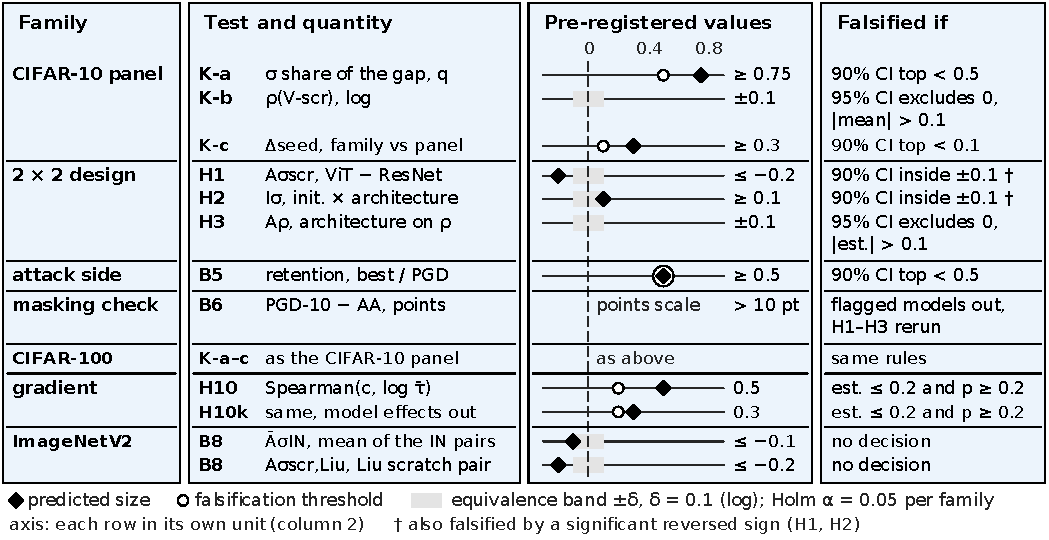
\includegraphics[width=\textwidth]{../figures/fig5_registry_map.pdf}
\caption{\textbf{Kayıtlı testler ve karar kuralları.} Satırlar Family sütununa göre gruplanmıştır. Test and quantity sütunu her testi adlandırmakta, Pre-registered values sütunu öngörülen büyüklüğü ve çürütme eşiğini eşdeğerlik bandıyla birlikte satırın kendi ölçeğine yerleştirmekte, Falsified if sütunu ise çürütme kuralını vermektedir. Holm düzeltmesi her aile içinde uygulanmış, ImageNetV2 satırları betimsel bırakılmıştır. B5, B6 ve B8 ön kayıt bloklarının etiketleridir.}
\label{fig:registry_map}
\end{figure*}

% ----------------------------------------------------------------------------
% 3.10 On kayit
% ----------------------------------------------------------------------------
\subsection{Ön Kayıt}
\label{subsec:prereg}

% FOY:M9.8:1684-1686 (betik, hucre tablosu, on kayit govdesi sha256);
% FOY:M10.6:2022-2032 (ek govde, hucre tablolari, ozgun ve catal betikler);
% FOY:M11.1:2078,2080 (K-a ve K-b hiyerarsik bootstrap: on kayitli, 31.10.2026'da sonradan uretildi);
% FOY:M11.2:2121 (S10-3: ek on kayit 6.4 kesifsel, sonradan uretildi); ONKAYIT_SAPMALAR.md satir 67-87;
% FOY:M9.8:1690, M9.9:1775 (ImageNet top-1 kayitta yok).
% KAYNAK: ON_KAYIT Sec. 1, 7, 8 (m.7, m.17), Dondurma eki (i) m.8;
% EK Sec. 1, 4.4, 5.7, 6.4, 12; R09 Sec. 0, 7; R11 Sec. 6 (beyanlar, brif
% Sec. 8.2). Uretilmeyenler: S9-2, S9-4, S8-1 (D_k, q_k), S8-3 grup
% jackknife, S8-7, S8-8, S10-1..S10-7, B10 her-ikisi-dogru Mantel.
Ana ön kayıt (panel testleri, $2\times2$ tasarım, saldırı tarafı, maskeleme) bu koşuların hiçbirinden önce, 29 Ekim 2026'da dondurulmuştur. Ön kayıt eki (CIFAR-100, ImageNetV2, gradyan hizalanması) ise matrislerinin ve gradyanlarının hiçbiri hesaplanmadan önce, 30 Ekim 2026'da dondurulmuştur (Şekil~\ref{fig:prereg_chain}). Ön kayıtlı testler dondurulmuş analiz betiğiyle, ön kayıt ekinin testleri ise bu betiği çağıran bir sarmalayıcıyla ve bir gradyan betiğiyle koşulmuştur. Bu iki betiğin özetleri ilk koşularından önce kayda geçirilmiştir. Dondurulmuş betiğin (\texttt{4bce2c983ace\ldots}), ek betiklerin, hücre tablolarının ve iki kayıt metninin SHA-256 özetleri, dondurma anında ya da ilk koşudan önce yazılan kayıtlarla ve analiz çıktılarında saklanan özetlerle örtüşmektedir. Ana ön kayıtta bir uygulama sapması bulunmaktadır. Dondurulmuş betikte K-a ve K-b için öngörülen hiyerarşik bootstrap duyarlılığına ait kod bulunmamaktadır. Bu analiz, dondurulmuş fonksiyonları değiştirmeden yükleyen ayrı bir betikle, sonuçlar ve bir iç değerlendirme görüldükten sonra iki CIFAR veri kümesinde hesaplanmıştır (Bölüm~\ref{subsec:panel}). Ön kayıt ekinde sapma yoktur ve bu eke ait keşifsel S10-3 analizi, yani aile göstergeli kısmi Mantel testi, bu noktada belirlenmiştir.

% FOY:M10.2:1842 (K-b(B9) eski yalniz pozitif okuma ile de curutme: evet)
Ön kayıttan önce görülen veriler test sayılmamaktadır. Bu veriler, Şekil~\ref{fig:prereg_chain} içindeki matrislerin yanı sıra havuz matrisi üzerindeki masa çözümlemelerini, $2\times2$ tasarım kodunun gerçek çift matrisleriyle yapılan bir deneme koşusunu ve küçük örneklemli duman testi matrisleri ile temiz doğrulukları kapsamaktadır. Deneme koşusu ve masa çözümlemesi, çiftin ViT'i ile 32 piksellik ResNet'i arasındaki $\sigma$ açığını zaten göstermişti ve H1 öngörüsü bu açık bilinerek yazılmıştır. H1'in bunun ötesinde sınadığı şey, ViT'in girdi hattındaki 224 piksellik bir ResNet-18'in açığın ResNet tarafını yeniden üretip üretmediğidir. Yeni bir hücrenin tam tarifli hiçbir koşusu görülmediğinden CIFAR-10 panel öngörüleri ilk tohumdaki gözlemi iki ek tohuma ve yedi üyeli bir panele genişletmektedir. Veri görüldükten sonra iki kural değişmiştir. K-b'nin çürütme ölçütü iki işarete genişletilmiş ve bu değişiklik çürütmeyi kolaylaştırmıştır. Bununla birlikte CIFAR-100'deki çürütme özgün tek yönlü kuraldan da çıkmaktadır. Bir yükleme denetimi olan temiz aşama denetimi ilk epoğa taşınmış ve \cellname{R224-IN} için referans olarak tek bir \cellname{R224-scr} koşusu alınmıştır. Hiçbir karar bu denetime bağlı değildir. Saldırı tarafı öngörüsünün momentum ve TGR duman testi matrislerinden önce yazılıp yazılmadığı dosya geçmişinden doğrulanamamaktadır. CIFAR-10 panel tablosunun yönlü değerlerine ön kayıt eki dondurulmadan önce bakılmış, ekin öngörüleri de dondurulmuş öngörülerden kopyalanmıştır. CIFAR-100 matrisi hesaplanırken bir başlatma betiği tek bir kaynağın günlük satırlarını ekrana basmış, analiz ise seçim bırakmayan tek bir çağrıdan oluşmaktadır.

Kayda geçirilmiş bazı duyarlılık ve keşifsel analizler üretilmemiştir. Bunlar arasında CIFAR-100'ün her ikisi doğru ve Hodge analizleri, ImageNetV2 ve gradyan analizlerinin bir kısmı ve her ikisi doğru Mantel testi bulunmaktadır. İki başlatma kontrol noktasının ImageNet top-1 doğruluğu kaydedilmemiştir.

% Sekil 6: paper/figures/fig6_prereg_chain.pdf (visio-cizici Uslup 8; yeni sekil Y5; results/q1/konsey_zaman_cizelgesi.json,
% foy M13 ve M9.8:1680-1686, kanit fig6_prereg_chain.kanit.json). Altyazidaki tek sayi takvim yili (Ekim 2026).
\begin{figure*}[!t]
\centering
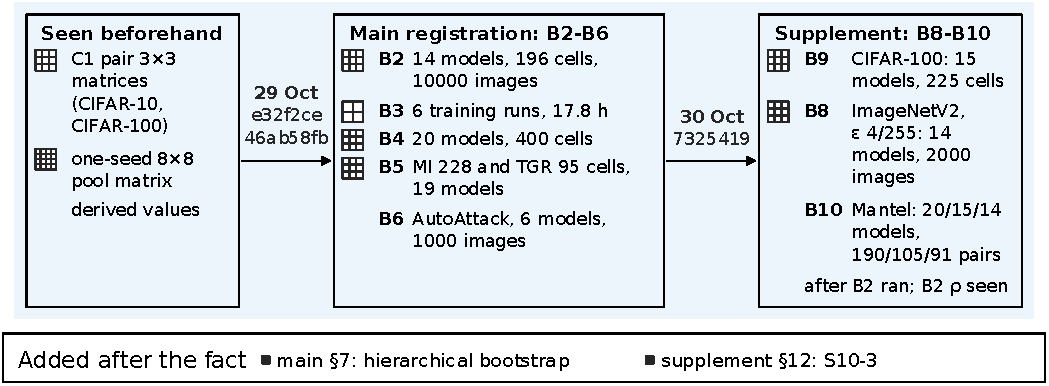
\includegraphics[width=\textwidth]{../figures/fig6_prereg_chain.pdf}
\caption{\textbf{Ön kayıt zinciri.} Seen beforehand şeridi ön kayıttan önce bakılan verileri listelemektedir. Main registration: B2-B6 şeridi ile metindeki ön kayıt ekine karşılık gelen Supplement: B8-B10 şeridi her bloğun modellerini, görüntülerini ve hücrelerini vermektedir. Oklar dondurma tarihlerini (Ekim 2026), sürüm kayıtlarını (commit) ve ön kayıt özetinin önekini taşımakta, Added after the fact şeridi ise sonuçlardan sonra üretilen iki analizi adlandırmaktadır.}
\label{fig:prereg_chain}
\end{figure*}

% ============================================================================
% BOLUM 4: DENEYLER
% ============================================================================
% 2026-10-04 (LeCun turu): EN 04_experiments.tex ile cumle duzeyinde esitlendi.
% Sira: A mutlak gurbuzluk -> B protokoller ve ozdeslik -> C kaynak etkisi ->
% D ayarlar arasi + yayilim/temiz fark sekli -> E standart hedefler ve dis havuz
% -> F secim kurali -> G uc okuma (gradyan, dikkat, TGR) -> H varyans kaynaklari.
% Karantina literalleri (eski Tablo 2 alt blogu, Tablo 3 dipnotu) cikarildi.
% Her sayi results/C1_REFERANS_FOYU.md'den.
\section{Deneyler}
\label{sec:experiments}

% ----------------------------------------------------------------------------
% A. Gurbuzluk karsilastirmasi
% ----------------------------------------------------------------------------
\subsection{Gürbüzlük Karşılaştırması}
\label{subsec:robustness}

Tablo~\ref{tab:main_results} mutlak gürbüzlüğü vermektedir. Bu çalışmada eğitilen modellere ait her hücre, mimari başına üç bağımsız eğitim koşusunun ortalaması ve bu koşular üzerindeki standart sapmadır; her koşu 10.000 örneklik tam test kümesinde değerlendirilmiştir.

\begin{table}[!t]
\centering
\caption{CIFAR-10'da ana gürbüzlük sonuçları ($\eps = 8/255$); mimari başına üç bağımsız eğitim koşusu üzerinden ortalama$\pm$std. AA, standart takımla AutoAttack anlamına gelmektedir.}
\label{tab:main_results}
\scriptsize
\setlength{\tabcolsep}{2pt}
\begin{tabular}{lcccccc}
\toprule
\textbf{Model} & \textbf{Savunma} & \textbf{Param.} & \textbf{Temiz} & \textbf{FGSM} & \textbf{PGD-10} & \textbf{AA} \\
\midrule
\multicolumn{7}{l}{\textit{CNN Modelleri}} \\
ResNet-18 & Yok & 11,2M & 95,25$\pm$0,15 & 40,29$\pm$1,77 & 0,03$\pm$0,03 & -- \\
ResNet-18 & AT & 11,2M & 85,78$\pm$0,36 & 53,46$\pm$0,08 & 44,11$\pm$0,50 & \textbf{37,93$\pm$0,14} \\
WRN-28-10 & AT$^\dagger$ & 36,5M & 89,48 & 70,91 & 66,92 & 62,76 \\
\midrule
\multicolumn{7}{l}{\textit{Görü Dönüştürücüsü Modelleri}} \\
ViT-Tiny & Yok & 5,7M & 80,09$\pm$0,60 & 6,10$\pm$1,47 & 0,05$\pm$0,05 & -- \\
ViT-Tiny & AT & 5,7M & 73,53$\pm$0,55 & 36,31$\pm$0,42 & 32,69$\pm$0,22 & \textbf{29,14$\pm$0,40} \\
\bottomrule
\multicolumn{7}{l}{\scriptsize $^\dagger$Gowal vd.'nin~\cite{gowal2020uncovering} RobustBench~\cite{croce2021robustbench} üzerinden dağıtılan gürbüz kontrol}\\
\multicolumn{7}{l}{\scriptsize \phantom{$^\dagger$}noktası; tek harici kontrol noktası olduğundan standart sapma yoktur.}\\
\multicolumn{7}{l}{\scriptsize \phantom{$^\dagger$}Temiz/FGSM/PGD-10: yerel tam test değerlendirmeleri; AA: RobustBench'in}\\
\multicolumn{7}{l}{\scriptsize \phantom{$^\dagger$}raporladığı değer (bu model üzerinde AutoAttack yeniden koşulmamıştır).}
\end{tabular}
\end{table}

CNN her saldırı altında \emph{mutlak} bir gürbüzlük üstünlüğü taşımaktadır: ResNet-18 AT, AutoAttack altında $\%37{,}93\pm0{,}14$ gürbüz doğruluğa ulaşırken ViT-Tiny AT $\%29{,}14\pm0{,}40$'ta kalmaktadır. Bir çiftin iki modeli de aynı 10.000 örnekte, örnek bazında kayıtla değerlendirildiğinden her koşu içinde McNemar'ın eşleştirilmiş testi uygulanabilmekte ve bu test üç çiftte de CNN lehine sonuç vermektedir (AutoAttack altında $p < 2\times10^{-84}$, PGD-10 altında $p < 2\times10^{-120}$). Çekişmeli eğitilmiş çiftte tohum düzeyindeki değişim raporlanan hiçbir doğrulukta 0,55 puanı aşmamaktadır; dolayısıyla sıralama koşudan koşuya gürültü değildir. CNN ayrıca daha yüksek bir temiz doğruluğu korumaktadır ($\%85{,}78$'e karşı $\%73{,}53$, 12,3 puanlık fark). Bu fark ViT'leri küçük veri kümelerinde sıfırdan eğitmenin güçlüğünü yansıtmaktadır; AutoAttack gürbüzlüğü de iki mimaride PGD-10'un altına düşmektedir (ResNet-18 için 6,2, ViT-Tiny için 3,6 puan). \%62{,}76'daki WideResNet-28-10 referansı~\cite{gowal2020uncovering}, kapasitenin, ek eğitim verisinin ve daha güçlü bir tarifin gürbüzlüğü mimari seçiminin ötesine birlikte ne kadar taşıdığını göstermektedir; bu model çalışma boyunca eşleşmiş çiftten ayrı tutulmaktadır.

\begin{table}[!t]
\centering
\caption{Tam test kümesinde beyaz kutu gürbüzlüğünün koşullu ayrıştırması; üç koşu üzerinden ortalama$\pm$std.}
\label{tab:conditional}
\scriptsize
\setlength{\tabcolsep}{2.5pt}
\begin{tabular}{lcccc}
\toprule
& \multicolumn{2}{c}{\textbf{Koşullu yanıltma (\%)}} & \multicolumn{2}{c}{\textbf{Her ikisi doğru gürbüz (\%)}} \\
\textbf{Model} & \textbf{PGD-10} & \textbf{AA} & \textbf{PGD-10} & \textbf{AA} \\
\midrule
ResNet-18 AT & \textbf{48,58}$\pm$0,80 & \textbf{55,78}$\pm$0,23 & \textbf{59,86}$\pm$0,35 & \textbf{51,89}$\pm$0,49 \\
ViT-Tiny AT & 55,53$\pm$0,50 & 60,37$\pm$0,33 & 46,11$\pm$0,59 & 41,15$\pm$0,39 \\
\bottomrule
\end{tabular}
\end{table}

Tablo~\ref{tab:conditional} mutlak skorları temiz doğruluk ve koşullu duyarlılık bileşenlerine ayırmaktadır (Bölüm~\ref{subsec:metrics}). Temizde yanlış sınıflandırılan girdiler gürbüz olmayan sayıldığından çarpanlara ayırma birebirdir ve AutoAttack için CNN'de $85{,}78 \times 0{,}442 = 37{,}93$, ViT'te $73{,}53 \times 0{,}396 = 29{,}14$ olarak okunmaktadır. İki çarpan da CNN lehinedir. CNN 12,3 puan daha yüksek bir temiz doğruluktan başlamakta \emph{ve} çözdüklerinin daha küçük bir kesrini kaybetmektedir; koşullu yanıltma PGD-10 altında $\%48{,}58$'e karşı $\%55{,}53$, AutoAttack altında $\%55{,}78$'e karşı $\%60{,}37$'dir. Çiftin iki modelinin de temizde doğru sınıflandırdığı $n=7.061\pm68$ örnekte, yani birebir eşleştirilmiş bir karşılaştırmada CNN 13,8 ve 10,7 puan öndedir (her koşuda McNemar $p<10^{-67}$; bu sınır söz konusu altkümede hesaplanmıştır ve yukarıda anılan tam küme sınırından zayıftır, aradaki fark büyük paydanın sağladığı kazançtır).

% 2026-10-04 (koordinator karari): onceki kontrol noktasi ciftinin sayilari (karantina)
% tablodan ve metinden cikarildi; yalniz nitel cumle kalir.
İki çarpanın aynı yönü göstermesi zorunlu olmadığından ayrıştırma, çarpanlar uyuştuğunda bile raporlanmaya değerdir. Sabit bölme protokolünden önce eğitilmiş ve temiz ön eğitimin zaten gördüğü bir doğrulama bölmesiyle seçilmiş daha eski bir kontrol noktası çifti aynı mutlak sıralamayı vermiş, ancak temiz doğruluk ile koşullu duyarlılık arasındaki payı farklı dağıtmıştır (Bölüm~\ref{subsec:training}). Bu türden bir atıf bu nedenle tek bir eğitim koşusundan çıkarılmamalıdır; tek başına raporlanan mutlak skor da işi hangi çarpanın yaptığını gizlemektedir.

Şekil~\ref{fig:epsilon_sweep}, $\eps \in \{2/255, 4/255, 8/255, 16/255\}$ bütçelerinde tam test kümesindeki PGD-10 gürbüz doğruluğunu göstermektedir.

\begin{figure}[!t]
\centering
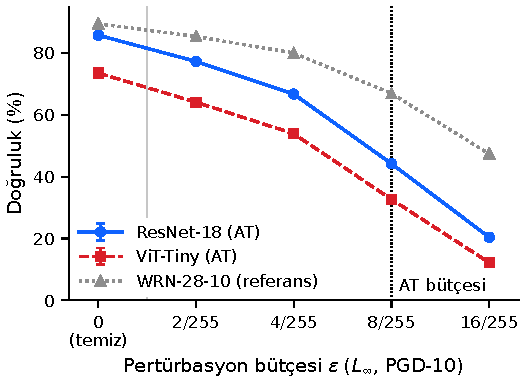
\includegraphics[width=\columnwidth]{../figures/final_tr/fig2_epsilon_sweep.pdf}
\caption{Pertürbasyon bütçesi $\eps$'a göre PGD-10 gürbüz doğruluğu, tam test kümesi (üç koşu ortalaması; $\pm$1 std hata çubukları işaretçilerden dardır). Yatay eksen kategoriktir ve $\eps=0$ temiz doğruluktur. Tarama ayrı bir PGD-10 değerlendirmesidir; bu yüzden $8/255$ noktası Tablo~\ref{tab:main_results}'den en çok $0{,}08$ puan ayrılır. CNN'in ViT üzerindeki marjı sabit değildir; küçük bütçelerde en geniş, $16/255$'te ise daralmış durumdadır.}
\label{fig:epsilon_sweep}
\end{figure}


% ----------------------------------------------------------------------------
% B. Protokoller ve ozdeslik
% ----------------------------------------------------------------------------
\subsection{Sabit Modeller Üzerinde Dört Koşullama Protokolü}
\label{subsec:transfer}

Her tohum çifti için PGD-10 çekişmeli örnekleri kaynak modelde üretilmiş ve tam test kümesinde bir hedef üzerinde değerlendirilmiştir. Sonuçlar örnek bazında kaydedildiğinden aynı saldırı koşusu, yeniden hesaplama gerekmeden Tablo~\ref{tab:protocol_masks}'teki her protokol altında puanlanabilmektedir; protokoller yalnızca paydaya hangi örneklerin girdiğinde ayrışmaktadır.

\begin{table}[!t]
\centering
\caption{Koşulsuz oran ve üç yerleşik koşullama protokolü altında transfer asimetrisi (PGD-10, $\eps$=8/255, tam test kümesi; üç tohum çifti üzerinden ortalama$\pm$std).}
\label{tab:transfer_protocols}
\footnotesize
\setlength{\tabcolsep}{3pt}
\begin{tabular}{lccc}
\toprule
\textbf{Protokol} & \textbf{CNN$\rightarrow$ViT} & \textbf{ViT$\rightarrow$CNN} & \textbf{Fark (puan)} \\
\midrule
Koşulsuz (ham) & 41,02$\pm$0,55 & 27,45$\pm$0,27 & $+$13,57$\pm$0,33 \\
Hedef doğru & 19,87$\pm$0,18 & 15,51$\pm$0,59 & $+$4,36$\pm$0,44 \\
Her ikisi doğru & 18,25$\pm$0,17 & 9,98$\pm$0,31 & $+$8,27$\pm$0,23 \\
Başarılı kaynak & 36,39$\pm$0,76 & 17,02$\pm$0,52 & $+$19,37$\pm$1,27 \\
\bottomrule
\end{tabular}
\end{table}

% Ic ice kosullama kumeleri sekli; TR surumu final_tr (surum 4: sag panelde uc ikili uzaklik).
\begin{figure}[!t]
\centering
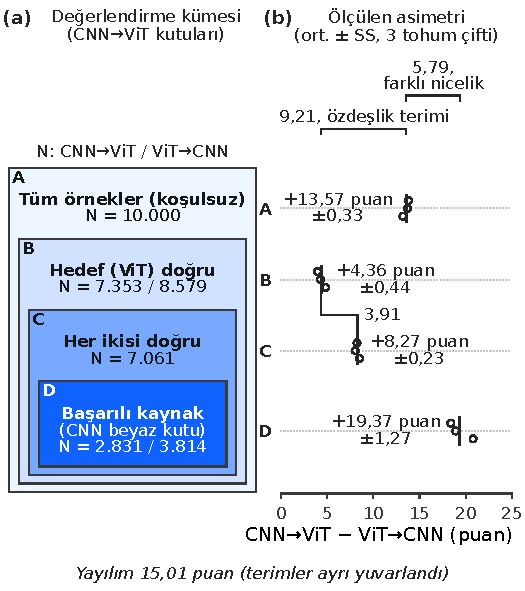
\includegraphics[width=\columnwidth]{../figures/final_tr/fig_protocol_sets.pdf}
\caption{Dört transfer protokolünün CNN$\rightarrow$ViT yönündeki iç içe değerlendirme kümeleri (a; kutular şematiktir ve alanla orantılı değildir, $N$ üç tohum çiftinin ortalamasıdır) ve her protokolün aynı modeller ve aynı veri üzerinde verdiği CNN$\rightarrow$ViT eksi ViT$\rightarrow$CNN asimetrisi (b; üç tohum çifti üzerinden çift içi eşleştirilmiş farkın ortalaması$\pm$SS, tek tek çiftler içi boş işaretçilerle). ViT$\rightarrow$CNN kümeleri aynı sırayla iç içedir ($N$ = 10.000, 8.579, 7.061 ve 3.814); koşulsuz ve her ikisi doğru kümeleri iki yönde aynıdır, diğer ikisi ise aynı değildir. (b) panelindeki bağlayıcılar üç ikili uzaklığı işaretlemektedir. CIFAR-10'da $15{,}01$ puanlık yayılım, başarılı kaynağın her ikisi doğru üzerindeki fazlası ($11{,}10$ puan, farklı bir nicelik) ile onaylanan ikili içindeki uzaklığın ($3{,}91$ puan) toplamıdır; koşulsuz kestirim bu aralığın içinde, Denklem~\eqref{eq:raw_identity}'in yerleştirdiği gibi hedef doğrunun $9{,}21$ puan üstünde yer almaktadır.}
\label{fig:protocol_sets}
\end{figure}

% REF: Tablo III: transfer protokolleri (N degerleri, 15.01 +- 0.84, ~4.4 kat)
% REF: Secim kuralinin asimetriye etkisi, B (kosumlar arasi araliklar 0.63 / 0.86 / 0.46 / 2.41)
Paydalar protokoller arasında keskin biçimde değişmektedir. CNN$\rightarrow$ViT ve ViT$\rightarrow$CNN için paydalar sırasıyla koşulsuz durumda 10.000/10.000, hedef doğruda 7.353/8.579, her ikisi doğruda 7.061 ortak örnek ve başarılı kaynakta 2.831/3.814'tür. Aynı modeller ve aynı veri üzerinde asimetri $+4{,}36\pm0{,}44$ ile $+19{,}37\pm1{,}27$ puan arasında değişmekte, uç değerler arasında 4,4 katlık bir oran bulunmakta ve en büyük ile en küçük protokol kestirimi arasındaki çift başına ortalama yayılım $15{,}01\pm0{,}84$ puan olmaktadır. Yeniden eğitim aynı niceliği çok daha az oynatmaktadır. Üç eğitim çifti boyunca asimetri, tablodaki sırayla dört protokol altında $0{,}63$, $0{,}86$, $0{,}46$ ve $2{,}41$ puanlık aralıklara yayılmaktadır; dolayısıyla benzeri benzeriyle, yani aralığı aralıkla karşılaştıran ölçüt $15{,}01$ puana karşı en çok $2{,}41$ puandır. Fark sütunundaki standart sapma ($0{,}23$ ile $1{,}27$ puan) çift içi eşleştirilmiş farka aittir ve iki yön çiftler boyunca birlikte değiştiği için yön başına yayılımlardan geri hesaplanamamaktadır.

% REF: Turetilmis, Protokol farklarinin farki (raw-tc +9.21+-0.76; ss-raw +5.79; ss-bc +11.10+-1.09; bc-tc +3.91+-0.32;
%      C100 raw-tc +13.58, bc-tc +5.97; L2 bc-tc +1.95; SVHN bc-tc +0.82 / +0.49)
% REF: Turetilmis, bc - tc kosum duzeyi %95 t araligi ([+3.12; +4.70]; C100 [+3.53; +8.40]; L2 [+1.33; +2.56])
Yayılım tek bir nicelik değildir. CIFAR-10'da yayılım bitişik protokoller arasındaki iki uzaklığa ayrılmaktadır (Şekil~\ref{fig:protocol_sets}b). Başarılı kaynak kestirimi kaynağın kendi beyaz kutu başarısızlığına koşullandığı için farklı bir niceliği, yani zaten işe yaramış bir saldırının ne ölçüde taşındığını kestirmektedir ve her ikisi doğru kestiriminin $11{,}10\pm1{,}09$ puan üstündedir. Yönlü iddialar için onaylanan ve yalnızca kaynağın da doğru olmasının gerekip gerekmediğiyle ayrışan iki protokol, hedef doğru ve her ikisi doğru, birbirinden $3{,}91\pm0{,}32$ puan uzaktadır; koşum düzeyindeki \%95 $t$ aralığı $[3{,}12;\ 4{,}70]$'tir (iki serbestlik derecesi). Bu uzaklık çözümleyicinin takdirinden değil iki farklı kestirilen nicelik arasındaki farktan doğmaktadır ve aşağıda betimlenen marjinal altkümeler onu açıklamaktadır. Her çiftte hedef doğru en küçük, başarılı kaynak en büyük kestirim olduğundan iki uzaklık birlikte $15{,}01$ puanlık aralığı oluşturmaktadır. Koşulsuz kestirim bu aralığın içinde, hedef doğrunun $9{,}21\pm0{,}76$ puan üstünde ve başarılı kaynağın $5{,}79$ puan altında yer almaktadır; hedeflerin temiz hataları, koşullu oranlar ve ölçülen öncül $p$ bilindiğinde Denklem~\eqref{eq:raw_identity} onu tam bu konuma yerleştirmektedir (Bölüm~\ref{subsubsec:matrix}). Onaylanan uzaklık CIFAR-100'de $5{,}97$ puan (aralık $[3{,}53;\ 8{,}40]$), $L_2$ bütçesi altında $1{,}95$ puan ($[1{,}33;\ 2{,}56]$), iki SVHN çiftinde ise $0{,}82$ ve $0{,}49$ puandır. CIFAR-100'de koşulsuz kestirim aralığın üst ucudur ve $13{,}58$ puanlık özdeşlik terimi $13{,}83$ puanlık yayılımın neredeyse tamamını oluşturmaktadır.

Protokol istatistiksel okumayı da değiştirmektedir. İki yönü aynı örnekler üzerinde puanlayan ve bu yüzden eşleştirilmiş çıkarımı destekleyen her ikisi doğru protokolünde fark $8{,}27\pm0{,}24$ puandır; bu değerin tablodaki $\pm0{,}23$'ten hafifçe ayrılmasının tek nedeni iki kestiricinin farklı olmasıdır. Her koşunun kendi eşleştirilmiş bootstrap güven aralığı vardır ($[7{,}61;\ 9{,}44]$, $[7{,}10;\ 9{,}01]$ ve $[7{,}28;\ 9{,}20]$). Uç noktaların ortalaması $[7{,}33;\ 9{,}22]$ aralığını vermektedir; bu aralık üç aralığın bir betimlemesidir ve kendi başına kapsama garantisi taşımamaktadır. Koşum düzeyinde çıkarım için koşumlar arası $t$ aralığı $[7{,}68;\ 8{,}86]$'dır. İşaret çevirme permütasyonunun $p$ değeri her tohumda $5\times10^{-5}$'in altındadır ve her aralık $\pm3$'ün tamamen dışında kaldığı için TOST üç marjın hiçbirinde ($\pm1$, $\pm2$ ve $\pm3$ puan) eşdeğerliği kuramamaktadır.

% REF: Turetilmis, Basarili-kaynak: siki ve gevsek okuma (+14.60; 10.45; +4.77+-0.39)
Protokol adları alt seçimleri de açık bırakmaktadır. Kaynağın temiz girdide zaten yanlış sınıflandırdığı örnekleri de içeri alan gevşek başarılı kaynak okumasında (Tablo~\ref{tab:protocol_masks}) ölçülen asimetri $+19{,}37$ puandan $+14{,}60$ puana, protokol yayılımı ise $15{,}01$ puandan $10{,}45$ puana inmektedir. Bu $4{,}77\pm0{,}39$ puanlık kayma, Tablo~\ref{tab:transfer_protocols}'teki herhangi bir protokolün koşumlar arası standart sapmasından üç kattan fazla büyüktür; diğer üç protokol ise yapısı gereği değişmemektedir.

CIFAR-10'da kararlı olan yöndür. CNN'de üretilen örnekler ViT'e, dört protokolün dördünde, üç tohumun üçünde ve momentum tabanlı MI-FGSM~\cite{dong2018boosting} altında da tersinden daha iyi transfer olmaktadır ($19{,}07\pm0{,}33$'e karşı $\%15{,}42\pm0{,}52$, hedef doğru; bu iki yönlü kontrol başka yerde kullanılan $\alpha=2/255$ yerine saldırının kendi varsayılan adımı olan $\alpha=\eps/10$'u kullanmaktadır ve ViT$\rightarrow$CNN değerinin Tablo~\ref{tab:tgr}'deki eşleşmiş bütçeli değerden hafifçe ayrılmasının nedeni budur). Dolayısıyla etki PGD saldırısının kendisinin bir artefaktı değildir. Etkinin büyüklüğü ve anlamlılığı, onlarla birlikte de her türlü eşdeğerlik iddiası protokole bağlıdır.

Onaylanan iki protokol arasındaki uzaklığın bileşimsel bir kaynağı vardır. Hedefin temizde çözdüğü ama kaynağın çözemediği örnekler ortak çözülenlerden üç-dört kat daha kırılgandır ($\%41{,}2\pm0{,}8$ ve $\%59{,}1\pm1{,}7$ yanıltmaya karşı $\%10{,}0$ ve $\%18{,}2$) ve bu marjinal altkümeler, iki model temiz doğrulukta ayrıştığı için boyutça beş kat farklıdır ($1.517\pm102$'ye karşı $291\pm16$). Hedef doğru koşullaması iki marjinal altkümeyi de içeri almakta ve bunların asimetrik boyutları iki oranı birbirine doğru çekmektedir; her ikisi doğru koşullaması ise onları dışarıda bırakmakta ve yönlü fark yeniden ortaya çıkmaktadır. Bu açıklama dört protokolün üçünü kapsamaktadır. Başarılı kaynak protokolü \emph{kaynağın} kendi gürbüzlüğüne göre seçim yapmaktadır; bu gürbüzlük çiftin temiz doğruluk farkının bir fonksiyonu olmadığından protokol ikinci, kısmen ters yönlü bir terim katmaktadır (Bölüm~\ref{subsubsec:spread_gap}).

% ----------------------------------------------------------------------------
% B.1 Uc mimarili kontrol ve oncul p
% ----------------------------------------------------------------------------
\subsubsection{Ham oranın ne kadarı hedefin temiz hatası?}
\label{subsubsec:matrix}

% REF: C3: WRN dahil 3x3 matris (r = 0.997; egim 0.762)
% REF: Dis veri: Mahmood, "Ozdeslikte kullanilan p" (p_min 0.989014, results/q1/ozdeslik_kontrol.json)
WideResNet-28-10 referansının hem kaynak hem hedef olarak eklenmesi her eğitim çifti için bir $3\times3$ matris vermektedir (Tablo~\ref{tab:transfer_matrix}); Denklem~\eqref{eq:raw_identity} bu matrisin altı köşegen dışı yönünde, temiz hataları birbirinden çok farklı hedeflere karşı sınanabilmektedir. Özdeşliğin öncülü bu çekişmeli eğitilmiş hedeflerde sıkı biçimde sağlanmaktadır. $36$ köşegen dışı yönde (iki veri kümesi, üç tohum çifti, üç hedef, iki kaynak) ölçülen $p$ değeri $0{,}989$ ile $1{,}000$ arasındadır. Bu nedenle $p=1$ biçimi ölçülen her koşulsuz oranı $0{,}41$ puan içinde yeniden üretmektedir; ortalama mutlak artık $0{,}095$ puandır ve artık, açıkladığı sapmanın en çok $\%1{,}39$'u kadardır. Bu artık puan cinsinden yeniden yazılmış öncül, yani $e\,(1-p)$ olduğundan ikinci bir doğrulama sayılmamaktadır; bilgi taşıyan nicelik $p$'nin kendisidir. Aynı sonuç sapma ile hedefin temiz hatası arasındaki bir korelasyon olarak ifade edilseydi ($r = 0{,}997$) eksik anlatılmış olurdu, çünkü bir niceliğin kendi baskın bileşeniyle bire yakın korelasyonu aritmetiktir.

Veri kümesine özgü kalan şey orantı çarpanıdır. $(1 - r_{\text{koş}})$ saldırının ne kadar transfer edilebilir olduğuna bağlı olduğundan uydurulan eğim CIFAR-10'da hedef hatasının puanı başına $0{,}762$, CIFAR-100'de $0{,}656$ puandır. Bu eğim ölçülen hedefler üzerinden bir ortalamadır ve özdeşlik başka model havuzlarına her uygulandığında yeniden kestirilmelidir. Koşulsuz transfer oranları bu yüzden mimariler arası transfer edilebilirliği ölçmemekte, transfer edilebilirliği hedefin temiz zayıflığıyla birlikte, Denklem~\eqref{eq:raw_identity}'in açıkça gösterdiği bir oranda ölçmektedir.

\begin{table}[!t]
\centering
\caption{$3\times3$ transfer matrisi (PGD-10, $\eps$=8/255, tam test kümesi; üç tohum çifti üzerinden ortalama$\pm$std; WideResNet satır ve sütunu tek harici kontrol noktasını kullanır). Ham = koşulsuz yanıltma oranı, Koş. = hedef doğru koşullu oran. Köşegen girdileri beyaz kutu saldırılardır. Bu matrisin saldırıları ayrı bir koşuda üretilmiştir (saldırı tohumu 42); Tablo~\ref{tab:conditional} ve Tablo~\ref{tab:transfer_protocols} ile paylaştığı hücreler onlardan en çok $0{,}06$ puan ayrılır ve bu fark Bölüm~\ref{subsec:statistics_results}'teki saldırı başlatma varyansının içindedir.}
\label{tab:transfer_matrix}
\footnotesize
\setlength{\tabcolsep}{3pt}
\begin{tabular}{llcc}
\toprule
\textbf{Kaynak} & \textbf{Hedef} & \textbf{Ham (\%)} & \textbf{Koş.\ (\%)} \\
\midrule
ResNet-18 AT & ResNet-18 AT & 55,84$\pm$0,53 & 48,52$\pm$0,84 \\
ResNet-18 AT & ViT-Tiny AT & 41,07$\pm$0,58 & 19,93$\pm$0,20 \\
ResNet-18 AT & WRN-28-10 & 21,69$\pm$0,09 & 12,48$\pm$0,10 \\
ViT-Tiny AT & ResNet-18 AT & 27,45$\pm$0,34 & 15,52$\pm$0,64 \\
ViT-Tiny AT & ViT-Tiny AT & 67,34$\pm$0,18 & 55,57$\pm$0,44 \\
ViT-Tiny AT & WRN-28-10 & 18,25$\pm$0,12 & 8,65$\pm$0,14 \\
WRN-28-10 & ResNet-18 AT & 32,63$\pm$0,14 & 21,48$\pm$0,31 \\
WRN-28-10 & ViT-Tiny AT & 39,73$\pm$0,25 & 18,15$\pm$0,28 \\
WRN-28-10 & WRN-28-10 & 33,03 & 25,16 \\
\bottomrule
\end{tabular}
\end{table}

% ----------------------------------------------------------------------------
% C. Kaynak etkisi
% ----------------------------------------------------------------------------
\subsection{Hedef Zayıflığı Değil, Kaynak Etkisi}
\label{subsec:source_target}

Üç mimarili $3\times3$ matrisler yönün nereden geldiğini de göstermektedir. Bir CNN$\rightarrow$ViT üstünlüğü, CNN'de üretilen örneklerin herhangi bir hedefe daha iyi taşınmasından, yani bir kaynak etkisinden ya da ViT'in herhangi bir kaynak için daha kolay hedef olmasından, yani bir hedef etkisinden doğabilir. İki etki, her eğitim çiftinin altı köşegen dışı oranına protokol protokol uydurulan ve toplamı sıfır kodlama kullanan $r(s\rightarrow t) = \mu + \alpha_s + \beta_t + \varepsilon_{st}$ toplamsal modeliyle ayrılmıştır. Böylece asimetri, kaynak farkı $\alpha_{\text{CNN}} - \alpha_{\text{ViT}}$, hedef farkı $\beta_{\text{ViT}} - \beta_{\text{CNN}}$ ve bir artık farkının toplamına eşit olmaktadır. Altı hücre ve beş parametre tek bir artık serbestlik derecesi bıraktığından yüksek bir $R^2$ beklenen bir sonuçtur ve az kanıt taşımaktadır; uydurma her matrisi betimlemekte, hiçbir şeyi sınamamaktadır, aşağıdaki sabit üçüncü model karşıtlıkları ise hiçbir model gerektirmemektedir.

% REF: Kaynak-hedef toplamsal ayristirma, CIFAR-10 ve CIFAR-100 cift basina ayristirma (tc, bc, ss, ham)
% REF: Kaynak-hedef toplamsal ayristirma, sabit-WRN karsitliklari; C3: WRN dahil 3x3 matris (gelen transfer; r = 0.986)
Kaynak terimi asimetriyi iki veri kümesinde de taşımaktadır (Tablo~\ref{tab:source_target}). CIFAR-10'da kaynak farkı $+5{,}13\pm0{,}09$, hedef farkı $-2{,}03\pm0{,}51$ puandır. ViT üzerinde üretilen örnekler daha kötü taşınmakta ve ViT iki hedefin \emph{daha az} kırılgan olanı olmaktadır; dolayısıyla hedef terimi ölçülen $+4{,}41\pm0{,}45$ puanlık asimetriye karşı çalışmaktadır. CIFAR-100 aynı örüntüyü daha büyük ölçekte yinelemektedir ($+9{,}54\pm0{,}64$'e karşı $-6{,}19\pm0{,}93$). Kaynak terimi puanlanabilen her protokolde işaretini korurken hedef terimi korumamaktadır. Her ikisi doğru protokolünde hedef farkı CIFAR-10'da sıfırdan ayırt edilemeyen $-0{,}53\pm0{,}59$, CIFAR-100'de $-2{,}85\pm0{,}93$ olurken kaynak farkı $+6{,}76\pm0{,}35$ ve $+11{,}79\pm0{,}83$'e çıkmaktadır; CIFAR-100 kayıtlarının izin verdiği başarılı kaynak protokolünde ise terimler $+20{,}82\pm1{,}43$ ve $-8{,}12\pm2{,}23$'tür. WideResNet aynı karşıtlıkları model gerektirmeden sağlamaktadır. Sabit bir hedef olarak WideResNet, ResNet'te üretilen örneklerin $\%12{,}48$'i, ViT'te üretilenlerin ise $\%8{,}65$'i ile kandırılmaktadır; yani ViT'te üretilen örnekler üçüncü bir mimariye bile daha kötü taşınmaktadır. Sabit bir kaynak olarak ise ResNet'i $\%21{,}48$, ViT'i $\%18{,}15$ oranında kandırmaktadır; dolayısıyla ViT üçüncü bir modelin pertürbasyonları için de daha zor hedeftir. Sabit model karşıtlıkları her ikisi doğru protokolünde de bu işaretleri korumakta (CIFAR-10'da $+4{,}69\pm0{,}38$ ve $-2{,}60\pm0{,}72$), hedef karşıtlığı ise iki veri kümesinde de her koşullu protokolde negatif kalmaktadır. Ham oranlarla puanlandığında aynı ayrıştırma CIFAR-10'da $+8{,}13$, CIFAR-100'de $+10{,}72$ puanlık bir hedef farkı vermektedir; koşulsuz oranlar ViT'in daha büyük temiz hatasını da saydığı için onu daha zayıf hedef gibi göstermektedir. Daha zayıf hedef okuması gelen transfer korelasyonuna da dayandırılamaz. Gelen koşullu transfer her hedefin kendi beyaz kutu koşullu yanıltma oranını izlemektedir (üç hedef üzerinde $r = 0{,}986$), ancak bu korelasyonu iki aileden gelen saldırıları da soğuran gürbüz WideResNet taşımaktadır ($\%10{,}57$ gelen transfer). ResNet ile ViT arasında gelen transfer yalnızca $0{,}54$ puan farklıdır ($\%18{,}50$'ye karşı $\%19{,}04$), asimetri ise $4{,}41$ puandır.

% REF: Kaynak-hedef toplamsal ayristirma, Mahmood ve ark. (2021) CIFAR-10 ve CIFAR-100 8x8 uydurmalari
% REF: Dis veri: Mahmood ve ark., Aile duzeyi asimetri ve guclu kaynak ailesi sayimi (12/12; 6/6)
Mahmood vd.'nin~\cite{mahmood2021robustness} $8\times8$ matrisleri, başka yerde eğitilmiş modeller üzerinde aynı ayrıştırmaya imkân vermektedir. Bu matrisler kendi her ikisi doğru protokolleri altında, çift başına $m=1000$ örnekle ve her hücrede FGSM, PGD ve MIM saldırılarının en güçlüsüyle ($\eps=0{,}031$) elde edilmiştir. Mahmood vd.'nin rejimi bu karşılaştırma için önemli olan her bakımdan buradakinden farklıdır. ViT ve BiT-M modelleri ImageNet-21k üzerinde ön eğitilmiş ve çekişmeli eğitim olmadan ince ayarlanmış, ResNet-56 ve ResNet-164 ise CIFAR üzerinde çekişmeli eğitim olmadan eğitilmiştir; köşegenleri de beyaz kutu saldırısı değil aynı modelin bağımsız eğitilmiş bir kopyası olduğundan dışarıda bırakılmıştır. Aile içi transfer aileler arası transferden çok daha güçlü olduğu için toplamsal model bu matrislere zayıf uymaktadır (CIFAR-10'da $R^2=0{,}368$, CIFAR-100'de $0{,}451$); aynı aile terimi $R^2$'yi $0{,}785$ ve $0{,}843$'e çıkarmaktadır. İki uydurmada da aile düzeyindeki kaynak farkı CIFAR-10'da ViT lehinedir (CNN eksi ViT olarak toplamsal uydurmada $-25{,}01$, aile terimiyle $-10{,}78$ puan) ve buradaki yönün tersini göstermektedir; melez ViT-R50'nin dışarıda bırakıldığı $12$ aileler arası çiftin tamamında da ViT daha güçlü kaynaktır. CIFAR-100'de ResNet-56 ve ResNet-164 bu çalışmanın yönünü göstermekte ve $6/6$ çiftte CNN$\rightarrow$ViT daha güçlü olmaktadır; ancak bu yönü hedef terimi taşımakta (toplamsal $+30{,}15$, aile terimiyle $+16{,}81$), kaynak terimi ise yine ViT lehine kalmaktadır ($-21{,}90$ ve $-8{,}55$). Orada yön buradakiyle uyuşmakta, mekanizma ise uyuşmamaktadır. Bölüm~\ref{subsec:findings} bu durumun açık bıraktığı soruyu tartışmaktadır.

% REF: tablo hucrelerinin tamami "Kaynak-hedef toplamsal ayristirma" ve "Dis veri: Mahmood ve ark." bolumlerinden.
\begin{table*}[!t]
\centering
\caption{Transfer matrislerinin toplamsal kaynak-hedef ayrıştırması (puan; köşegen dışı hücreler). Kaynak farkı $=\alpha_{\text{CNN}}-\alpha_{\text{ViT}}$ (pozitif değer CNN'de üretilen örneklerin daha iyi taşındığını gösterir); hedef farkı $=\beta_{\text{ViT}}-\beta_{\text{CNN}}$ (pozitif değer ViT'in daha kırılgan hedef olduğunu gösterir); asimetri $=$ CNN$\rightarrow$ViT eksi ViT$\rightarrow$CNN. Üst blok: bu çalışmanın $3\times3$ matrisleri (ResNet-18 AT, ViT-Tiny AT, WideResNet-28-10; standart eğitilmiş satırda her çiftin temiz eğitilmiş ResNet-18 ve ViT-Tiny modelleri ile RobustBench'in standart WideResNet-28-10 modeli), eğitim çifti ve protokol başına uydurulmuş, üç çift üzerinden ortalama$\pm$std. Matrisler Tablo~\ref{tab:transfer_matrix}'deki ayrı saldırı koşusundan geldiği için CIFAR-10 hedef doğru asimetrisi burada $4{,}41$, Tablo~\ref{tab:transfer_protocols}'te $4{,}36$'dır; altı hücre ve beş parametreyle $R^2$ sınamaz, yalnızca betimler. Orta blok: uydurma yapılmadan sabit üçüncü model olarak WideResNet; hedef olarak bir kaynak karşıtlığı (CNN'den gelen oran eksi ViT'ten gelen oran), kaynak olarak bir hedef karşıtlığı (ViT'e giden oran eksi CNN'e giden oran) verir. Alt blok: Mahmood vd.'nin~\cite{mahmood2021robustness} $8\times8$ her ikisi doğru matrisleri (standart eğitilmiş modeller, $m$=1000, köşegen hariç); aksi belirtilmedikçe melez ViT-R50 dışındaki CNN ve ViT aileleri, aynı aile terimli ve terimsiz uydurmalar.}
\label{tab:source_target}
\footnotesize
\setlength{\tabcolsep}{4pt}
\begin{tabular}{llccccc}
\toprule
\textbf{Veri} & \textbf{Protokol ya da uydurma} & \textbf{Kaynak farkı} & \textbf{Hedef farkı} & \textbf{Asimetri} & \textbf{En büyük $|$artık$|$} & \textbf{$R^2$} \\
\midrule
\multicolumn{7}{l}{\textit{Bu çalışmanın matrisleri, eğitim çifti başına toplamsal uydurma}} \\
CIFAR-10 & Hedef doğru & $+$5,13$\pm$0,09 & $-$2,03$\pm$0,51 & $+$4,41$\pm$0,45 & 0,65$\pm$0,05 & 0,9782$\pm$0,0032 \\
CIFAR-10 & Her ikisi doğru & $+$6,76$\pm$0,35 & $-$0,53$\pm$0,59 & $+$8,30$\pm$0,16 & 1,04$\pm$0,11 & 0,9643$\pm$0,0072 \\
CIFAR-10 & Koşulsuz & $+$4,47$\pm$0,10 & $+$8,13$\pm$0,33 & $+$13,62$\pm$0,38 & 0,51$\pm$0,03 & 0,9964$\pm$0,0004 \\
CIFAR-100 & Hedef doğru & $+$9,54$\pm$0,64 & $-$6,19$\pm$0,93 & $+$4,96$\pm$1,02 & 0,80$\pm$0,05 & 0,9871$\pm$0,0015 \\
CIFAR-100 & Her ikisi doğru & $+$11,79$\pm$0,83 & $-$2,85$\pm$0,93 & $+$10,92$\pm$0,34 & 0,99$\pm$0,10 & 0,9851$\pm$0,0035 \\
CIFAR-100 & Başarılı kaynak & $+$20,82$\pm$1,43 & $-$8,12$\pm$2,23 & $+$17,50$\pm$0,92 & 2,40$\pm$0,06 & 0,9830$\pm$0,0008 \\
CIFAR-100 & Koşulsuz & $+$6,48$\pm$0,38 & $+$10,72$\pm$0,97 & $+$18,53$\pm$0,71 & 0,67$\pm$0,01 & 0,9946$\pm$0,0003 \\
C10, standart eğitim & Hedef doğru & $+$69,18$\pm$2,31 & $-$75,05$\pm$1,72 & $-$4,49$\pm$0,85 & 0,69$\pm$0,20 & 0,9996$\pm$0,0002 \\
\midrule
\multicolumn{7}{l}{\textit{Sabit üçüncü model olarak WideResNet-28-10, uydurma yok}} \\
CIFAR-10 & Hedef doğru & $+$3,83$\pm$0,17 & $-$3,33$\pm$0,59 & -- & -- & -- \\
CIFAR-10 & Her ikisi doğru & $+$4,69$\pm$0,38 & $-$2,60$\pm$0,72 & -- & -- & -- \\
CIFAR-100 & Hedef doğru & $+$7,94$\pm$0,54 & $-$7,79$\pm$0,95 & -- & -- & -- \\
CIFAR-100 & Her ikisi doğru & $+$9,81$\pm$1,03 & $-$4,83$\pm$0,75 & -- & -- & -- \\
CIFAR-100 & Başarılı kaynak & $+$16,03$\pm$1,42 & $-$12,91$\pm$2,29 & -- & -- & -- \\
C10, standart eğitim & Hedef doğru & $+$67,80$\pm$2,11 & $-$76,43$\pm$2,02 & -- & -- & -- \\
\midrule
\multicolumn{7}{l}{\textit{Mahmood vd.~\cite{mahmood2021robustness}, $8\times8$ her ikisi doğru matrisler, aile düzeyi}} \\
CIFAR-10 & Toplamsal & $-$25,01 & $+$2,08 & $-$24,01 & 74,04 & 0,3681 \\
CIFAR-10 & Aynı aile terimi & $-$10,78 & $-$12,15 & $-$24,01 & 29,33 & 0,7852 \\
CIFAR-100 & Toplamsal & $-$22,77 & $+$14,74 & $-$9,02 & 66,29 & 0,4508 \\
CIFAR-100 & Aynı aile terimi & $-$9,43 & $+$1,39 & $-$9,02 & 24,33 & 0,8425 \\
CIFAR-100 & ResNet-56/164 ile ViT, toplamsal & $-$21,90 & $+$30,15 & $+$9,15 & -- & -- \\
CIFAR-100 & ResNet-56/164 ile ViT, aynı aile & $-$8,55 & $+$16,81 & $+$9,15 & -- & -- \\
\bottomrule
\end{tabular}
\end{table*}

% ----------------------------------------------------------------------------
% D. Ayarlar arasi
% ----------------------------------------------------------------------------
\subsection{Veri Kümeleri ve Tehdit Modelleri Arasında}
\label{subsec:settings}

Tablo~\ref{tab:protocol_settings} bu makaledeki her ayarda dört protokolü bir araya getirmektedir. Onaylanan iki protokol her ayarın içinde aynı işareti vermektedir; protokoller arasında işaret yalnızca SVHN'de değişmekte ve orada dört kestirimin tamamı sıfırın üç puan yakınında kalmaktadır. Ayarlar aşağıda sırayla ele alınmakta (Bölüm~\ref{subsec:cifar100} ile~\ref{subsec:l2} arası), ardından ölçülen her çiftte yayılım ile temiz doğruluk farkı arasındaki ilişki incelenmektedir (Bölüm~\ref{subsubsec:spread_gap}).

% ----------------------------------------------------------------------------
% D.1 Ikinci veri kumesi (E1)
% ----------------------------------------------------------------------------
\subsubsection{İkinci bir veri kümesi: CIFAR-100}
\label{subsec:cifar100}

Yalnızca CIFAR-10'da var olan bir protokol etkisi genel bir raporlama önerisini desteklemeyeceği için tasarımın tamamı CIFAR-100 üzerinde yinelenmiştir; mimariler, tehdit modeli, saldırı bütçesi, üç tohumlu yapı ve dört protokol aynı tutulmuştur. Üç yönsel ön kestirim ile üç uç nokta bandı, bu veri kümesinden herhangi bir ölçüm mevcut olmadan önce salt eklemeli bir belgeye kaydedilmiş, böylece sonucun ölçüldükten sonra yeniden yorumlanmasının önüne geçilmiştir. Kayıt eğitimin başlangıcından önce gelmemektedir; kayıt işlemesi, sayı bildiren ilk adımdan, yani epok 5'teki pilot kapısından altmış altı dakika öncedir.

\begin{table}[!t]
\centering
\caption{CIFAR-100 yinelemesi (mimari başına üç bağımsız eğitim koşusunun ortalaması$\pm$std, tam test kümesi, $\eps$=8/255). İki model de Bölüm~\ref{subsec:training}'deki tarifle eğitilmiştir. Mutlak gürbüzlük iki mimaride de CIFAR-10'a göre düşüktür ve CNN'in ViT üzerindeki sıralaması değişmemiştir.}
\label{tab:cifar100_results}
\footnotesize
\begin{tabular}{lccc}
\toprule
\textbf{Model} & \textbf{Temiz (\%)} & \textbf{PGD-10 (\%)} & \textbf{AutoAttack (\%)} \\
\midrule
ResNet-18 AT & 63,86$\pm$1,05 & 19,30$\pm$0,32 & 15,04$\pm$0,54 \\
ViT-Tiny AT  & 43,17$\pm$1,10 & 11,15$\pm$0,60 & 8,87$\pm$0,83 \\
\bottomrule
\end{tabular}
\end{table}

Mutlak gürbüzlük CIFAR-10'a göre düşüktür ve CNN'in ViT üzerindeki sıralamasını korumaktadır (Tablo~\ref{tab:cifar100_results}). Aynı dört protokol boyunca ölçülen CNN$\rightarrow$ViT asimetrisi $+4{,}96\pm1{,}01$ puandan (hedef doğru) $+18{,}53\pm0{,}71$ puana (koşulsuz) uzanmakta; her ikisi doğru protokolünde $+10{,}92\pm0{,}34$, başarılı kaynak protokolünde ise $+17{,}50\pm0{,}92$ puan olmaktadır. Tohum başına ortalama yayılım $13{,}83\pm1{,}30$ puandır; CIFAR-10'da bu değer $15{,}01\pm0{,}84$ olduğuna göre daha zor veri kümesi protokol etkisini aynı aralıkta, CIFAR-10 değerinin bir miktar altında bırakmaktadır. Yön, CIFAR-10'da olduğu gibi on iki ölçümün tamamında pozitiftir (dört protokol $\times$ üç tohum çifti). Her ikisi doğru protokolünde eşleştirilmiş fark $10{,}92$ puandır. CIFAR-10'da olduğu gibi verilen $[9{,}47;\ 12{,}35]$ aralığı üç tohumun kendi bootstrap uç noktalarının ortalamasıdır ve kapsama garantisi taşımamaktadır; mimarilere ilişkin bir iddiayla eşleşen koşumlar arası $t$ aralığı ise $[10{,}07;\ 11{,}77]$'dir. İşaret çevirme permütasyonunun $p$ değeri her tohumda $20.000$ permütasyonun çözünürlüğünün altındadır ve TOST sınanan hiçbir marjda eşdeğerliği kuramamaktadır.

Kaydedilen üç ön kestirimin biri doğrulanmış, biri bağlayıcı kabul edilen okumada tutmamış, üçüncüsü ise bu tasarımda sınanamamıştır. İşaretin korunacağı ön kestirimi doğrulanmıştır ($12/12$). Protokol yayılımının daha zor veri kümesinde büyüyeceği ön kestirimi CIFAR-10 yayılımına karşı bir karşılaştırma olarak kaydedilmiş ve o tarihte bu yayılım $10{,}45$ puan olarak anılmıştı. Bu sayısal eşiğe karşı kestirim tutmaktadır ($13{,}83 > 10{,}45$); sıkı başarılı kaynak okuması altındaki güncel CIFAR-10 yayılımına karşı ise tutmamaktadır ($13{,}83 < 15{,}01$). Kayıt sayıyı değil CIFAR-10 yayılımını adlandırdığı için bu sonuç bir başarısızlık olarak sayılmıştır. Üçüncü ön kestirim, koşulsuz oranın koşullu orandan sapmasının hedefin temiz hatasıyla birlikte büyüyeceğini öngörüyordu. Ölçülen eğim hedef hatasının puanı başına $+0{,}656$ puandır ve öngörüldüğü gibi pozitiftir. Ancak CIFAR-100'de üç hedeften ikisinin temiz hatası yalnızca $0{,}21$ puan farklıdır ($36{,}15$ ve $36{,}36$); dolayısıyla korelasyon üç değil iki etkin küme üzerinden hesaplanmakta ve değeri (altı yön üzerinde $r = 0{,}931$, hedef düzeyinde $0{,}974$) iki noktalı bir karşıtlığa dayanmaktadır. Ölçüm ön kestirimi \emph{sınamadan} onunla \emph{tutarlıdır} ve üçüncü bir doğrulama sayılmamaktadır.

Kaydedilen uç noktalardan biri tutmamıştır. Çekişmeli eğitilmiş ViT için temiz doğruluk $\%33$ ile $40$ bandında öngörülmüş, $\%43{,}17\pm1{,}10$ ölçülmüştür. Bant, çekişmeli eğitimin temiz doğruluk bedelinin iki mimaride aynı biçimde ölçekleneceği varsayımıyla türetilmişti. Bu varsayım tutmamıştır; ViT çekişmeli eğitim altında temiz ön eğitim doğruluğunun $0{,}885$'ini korurken ResNet $0{,}802$'sini korumuştur. Protokol iddiasının dayandığı iki çekişmeli uç nokta ise bantlarının içinde kalmıştır (PGD-10 öngörüsü $\%10$ ile $14$, ölçüm $11{,}15$; AutoAttack öngörüsü $\%8$ ile $11$, ölçüm $8{,}87$). Koşullama sınıf karışımını da değiştirdiğinden bir asimetri ilke olarak bir bileşim artefaktı olabilirdi, ancak ölçümler bunu göstermemektedir. Hedef doğru protokolünde asimetrinin bileşim bileşeni üç tohum çiftinde $-1{,}249$, $-1{,}330$ ve $-1{,}065$ puandır ve \emph{negatiftir}; yani sınıf karışımı yeniden dengelenseydi asimetri büyürdü. Başarılı kaynak protokolünde bu bileşen küçüktür ve her tohumda pozitiftir ($+0{,}527$, $+0{,}435$ ve $+0{,}382$ puan); koşulsuz ve her ikisi doğru protokollerinde ise ayrıştırmanın gerektirdiği gibi tam olarak sıfırdır.

Bu sonuç iki niteleme taşımaktadır. Birincisi, iki çekişmeli bant en yakın tohum düzeyi kenarında $0{,}22$ puanlık (AutoAttack) ve $0{,}48$ puanlık (PGD-10) marjlarla tutmuştur ve bu marjlar aynı veri kümesindeki kontrol noktası seçimi gürültüsünden küçüktür. Eğitim koşusu sabit tutularak CIFAR-100 yörüngelerinde erken durdurma sabrı ve eğri yumuşatması tarandığında raporlanan PGD-10 doğruluğu $0{,}18$ ile $1{,}83$ puan arasında oynamaktadır (ortalama $0{,}86$). Aynı dokuz hücreli tarama CIFAR-10'da doğrulama bölmesi başına $0{,}54$ ile $2{,}83$ puan vermektedir; Bölüm~\ref{subsec:selection}'deki on sekiz hücreli değer ise bölmeyi de değiştirdiği için daha da büyüktür ve CIFAR-100 protokolünde bu boyut bulunmamaktadır. İkincisi, iki bağımsız bölme yerine aynı ayrılmış bölme iki aşamada da seçim için kullanılmıştır; bu tercih iki veri kümesini karşılaştırılabilir tutmak amacıyla CIFAR-10 protokolünden devralınmıştır.

% ----------------------------------------------------------------------------
% D.2 Ucuncu veri kumesi: SVHN, esleşmeye yakin cift
% ----------------------------------------------------------------------------
\subsubsection{Eşlenmeye yakın bir çiftle üçüncü bir veri kümesi: SVHN}
\label{subsec:svhn}

CIFAR-10 ve CIFAR-100 iki mimariyi temiz doğrulukta birbirinden hayli uzağa yerleştirmektedir (yaklaşık $12$ ve $21$ puan). SVHN~\cite{netzer2011reading} ise böyle değildir. Aynı tarifle çekişmeli eğitildiğinde ResNet iki koşuda $\%94{,}76$ ve $\%93{,}77$ (ortalama $94{,}27$), ViT ise $\%92{,}82$ ve $\%92{,}03$ (ortalama $92{,}42$) temiz doğruluğa ulaşmakta, aradaki farklar $1{,}94$ ve $1{,}74$ puan (ortalama $1{,}84$) olmaktadır. İki koşudan hesaplanan $0{,}70$ ve $0{,}56$'lık standart sapmalar az bilgi taşıdığından koşu değerleri ayrı ayrı verilmiştir. Ortalama gürbüz doğruluklar PGD-10 altında $\%55{,}52$ ve $\%52{,}30$'dur. PGD-10 farkı hâlâ yaklaşık üç puan olduğundan bu çift eşlenmiş değil, eşlenmeye yakın olarak adlandırılmaktadır. Özdeşlik terimi temiz doğruluk farkını izliyorsa burada yönün kendisi bir protokol meselesine dönüşmelidir.

\begin{table*}[!t]
\centering
\caption{Bu makaledeki her ayarda dört koşullama protokolü altında transfer asimetrisi (CNN$\rightarrow$ViT eksi ViT$\rightarrow$CNN, yüzde puan; PGD-10; $L_\infty$ altında $\eps$=8/255, $L_2$ altında $\eps$=0,5; tam test kümeleri). Üç tohum çiftli ayarlarda çiftler üzerinden ortalama$\pm$std verilir; SVHN'de iki çift olduğundan standart sapma yerine iki değer ayrı ayrı basılır. Yayılım, çift başına dört protokol üzerindeki açıklığın çiftler üzerinden ortalamasıdır. Onaylanan iki protokol, hedef doğru ve her ikisi doğru, her ayarın içinde aynı işareti verir; protokoller arasında işaret yalnızca SVHN'de değişir ve orada dört kestirimin tamamı sıfırın üç puan yakınındadır.}
\label{tab:protocol_settings}
\footnotesize
\begin{tabular}{lcccc}
\toprule
\textbf{Protokol} & \textbf{CIFAR-10, $L_\infty$} & \textbf{CIFAR-100, $L_\infty$} & \textbf{SVHN, $L_\infty$} & \textbf{CIFAR-10, $L_2$} \\
 & 3 çift, $n$=10.000 & 3 çift, $n$=10.000 & 2 çift, $n$=26.032 & 3 çift, $n$=10.000 \\
\midrule
Koşulsuz (ham) & $+$13,57$\pm$0,33 & $+$18,53$\pm$0,71 & $+$0,33 / $+$0,45 & $+$13,03$\pm$0,81 \\
Hedef doğru & $+$4,36$\pm$0,44 & $+$4,96$\pm$1,01 & $-$1,16 / $-$0,85 & $+$2,12$\pm$0,18 \\
Her ikisi doğru & $+$8,27$\pm$0,23 & $+$10,92$\pm$0,34 & $-$0,34 / $-$0,36 & $+$4,07$\pm$0,36 \\
Başarılı kaynak & $+$19,37$\pm$1,27 & $+$17,50$\pm$0,92 & $+$2,98 / $+$2,41 & $+$12,06$\pm$0,23 \\
\midrule
Yayılım (en büyük $-$ en küçük) & 15,01$\pm$0,84 & 13,83$\pm$1,30 & 4,14 / 3,26 & 10,92$\pm$0,82 \\
\bottomrule
\end{tabular}
\end{table*}

% REF: Transfer asimetrisi, dort protokol, ayarlar (SVHN satirlari; Her ikisi dogru, eslesmis analiz: SVHN)
Ölçümler bu beklentiyle uyuşmaktadır. Dört protokolün ikisi CNN, ikisi ViT üstünlüğü bildirmektedir (Tablo~\ref{tab:protocol_settings}). Yönlü iddialar için onaylanan iki protokol, hedef doğru ile her ikisi doğru, birbiriyle uyuşmakta ve ikisi de ViT lehine çıkmaktadır; işaret değişimi bu iki protokolü koşulsuz ve başarılı kaynak oranlarından ayırmaktadır. Koşulsuz orandaki çevrilme Denklem~\eqref{eq:raw_identity}'den aritmetik olarak çıkmaktadır. Burada ViT hedefinin temiz hatası CNN'inkini yaklaşık iki puan aşmakta ve bu fark $-1{,}00$'lık hedef doğru farkını $+0{,}39$'luk ham farka taşımaya yetmektedir. İki yönü özdeş örnekler üzerinde puanladığı için birincil kabul edilen her ikisi doğru protokolünde fark $-0{,}35$ puandır; işaret çevirme permütasyonunun $p$ değeri $0{,}105$'tir ve TOST eşdeğerliği, sınanan en dar marj ($\pm1$ puan) dahil üç marjın üçünde de kabul edilmektedir. Böyle bir eşdeğerlik iddiasının kurulup kurulamayacağına da protokol karar vermektedir. Ölçümden önce sabitlenen $\pm2$ marjında iki nokta kestirimi ($+2{,}98$ ve $+2{,}41$) marjın dışında kaldığı için hiçbir başarılı kaynak kestirimi bu sınamayı geçemezken, iki her ikisi doğru kestirimi ($-0{,}34$ ve $-0{,}36$) marjın rahatça içindedir. Kabul bir niteleme gerektirmektedir. SVHN iki tohum çiftiyle koşulduğundan verilen $[-0{,}76;\ +0{,}07]$ aralığı iki tohumun bootstrap uç noktalarının ortalamasıdır ve koşumlar arası bir aralık elde edilememektedir; eşdeğerlik koşum içi karşılaştırmaya ve iki koşumun yakın uyuşmasına dayanmakta, iki koşum ise koşumlar arası değişimi sınırlayamamaktadır. Yalnızca başarılı kaynak oranını raporlayan bir çalışma SVHN'de $2{,}70$ puanlık bir CNN üstünlüğü, yalnızca hedef doğru oranını raporlayan bir çalışma ise $1{,}00$ puanlık bir ViT üstünlüğü duyururdu.

SVHN'de dört protokollü yayılım iki çiftte $4{,}14$ ve $3{,}26$ puandır (ortalama $3{,}70$); bu değer CIFAR-10'da $15{,}01\pm0{,}84$, CIFAR-100'de $13{,}83\pm1{,}30$ puan iken temiz doğruluk farkları sırasıyla $1{,}84$, $\approx12$ ve $\approx21$ puandır. Özdeşlik terimine karşılık gelen üç protokollü yayılım ise $1{,}49$ ve $1{,}30$ puandır. İlişki üç veri kümesi arasında tekdüze değildir ve en büyük fark en büyük yayılımı vermemektedir. SVHN'i ayıran özellik eşlenmeye yakın çifttir. Yayılım yeterince küçüldüğünde asimetrinin kendisini aşamamakta ve işaret mimarilerin değil protokolün bir özelliği haline gelmektedir; Bölüm~\ref{subsec:transfer}'te kararlı olarak raporlanan yön, iki CIFAR veri kümesinin de bulunduğu \emph{iki modelin temiz doğrulukta ayrıştığı rejimde} kararlıdır. SVHN önceden sabitlenmiş indirgenmiş bir yapılandırmayla koşulmuştur; üç yerine iki tohum çifti kullanılmış, çekişmeli eğitim $50$ epokla sınırlanmış, AutoAttack ve üçüncü mimari yer almamıştır. Bu nedenle Bölüm~\ref{subsubsec:matrix}'teki $3\times3$ kontrol burada kurulmamıştır.

% ----------------------------------------------------------------------------
% D.3 Tehdit modelinin degistirilmesi
% ----------------------------------------------------------------------------
\subsubsection{İkinci bir tehdit modeli: $L_2$}
\label{subsec:l2}

Protokol etkisinin $\Linf$'ye özgü bir artefakt olup olmadığını sınamak için aynı CIFAR-10 kontrol noktaları $\eps=0{,}5$'lik bir $L_2$ bütçesi altında yeniden değerlendirilmiş ve üç yönsel ön kestirim herhangi bir $L_2$ çıktısına bakılmadan önce kaydedilmiştir. Modeller $\Linf$ ile eğitildiğinden bu ölçüm $L_2$ gürbüzlüğünü değil protokolün sonucu nasıl etkilediğini yoklamaktadır ve aşağıdaki mutlak değerler $L_2$ ile eğitilmiş referanslarla karşılaştırılamamaktadır.

\begin{table}[!t]
\centering
\caption{Aynı kontrol noktaları, $L_2$ bütçesi ($\eps$=0,5; üç tohum çiftinin ortalaması$\pm$std). PGD-L2 tam test kümesini, AutoAttack-L2 ise ölçümden önce sabitlenen $5.000$ örneklik bir altkümeyi kullanır; bu yüzden temiz sütunu tam küme değerinden bir miktar farklıdır ve ikisi aynı örneklerden gelmez.}
\label{tab:l2_results}
\footnotesize
\begin{tabular}{lcccc}
\toprule
\textbf{Model} & \textbf{Temiz} & \textbf{PGD-L2} & \textbf{Temiz (5k)} & \textbf{AA-L2} \\
\midrule
ResNet-18 AT & 85,78 & 63,78$\pm$0,38 & 85,33 & 60,61$\pm$0,42 \\
ViT-Tiny AT & 73,53 & 51,72$\pm$0,23 & 73,61 & 49,85$\pm$0,20 \\
\bottomrule
\end{tabular}
\end{table}

Norm değişince protokol yayılımı $10{,}92$ puana küçülmektedir ($\Linf$ altında $15{,}01$); ancak hem kayıtta belirlenen iki puanlık tabanın hem de koşumlar arası standart sapmanın çok üstünde kalmakta ve işaret on iki ölçümün tamamında pozitif çıkmaktadır; böylece kaydedilen ilk iki ön kestirim tutmaktadır. Dört protokolün (Tablo~\ref{tab:protocol_settings}) bildirdiği asimetriler $+13{,}03\pm0{,}81$ (koşulsuz), $+2{,}12\pm0{,}18$ (hedef doğru), $+4{,}07\pm0{,}36$ (her ikisi doğru) ve $+12{,}06\pm0{,}23$ puandır (başarılı kaynak). Üçüncü ön kestirim, yani koşulsuz oranın koşullu orandan sapmasının hedefin temiz hatasıyla artacağı, Denklem~\eqref{eq:raw_identity} sağlandığı sürece yanlışlanamaz ve uydurulan $+0{,}914$ eğimi bir şeyi sınamak yerine $1 - r_{\text{koş}}$'u kestirmektedir. On sekiz yön yalnızca yedi ayrık hedef hatası değeri aldığından ve bunların altısı aynı sabit WideResNet'ten geldiğinden korelasyon yerine eğim raporlanmaktadır. Ön kestirim özdeşlik yazılmadan önce kaydedilmişti ve şimdi özdeşliğin örneklem dışı bir sınaması işlevini görmektedir. Eğim de özdeşliğin öngördüğü yerde durmaktadır. Koşullu oranlar bu $L_2$ bütçesi altında $\Linf$'dekinden çok daha düşük olduğundan (kabaca $\%2$ ile $9$'a karşı $\%9$ ile $22$) özdeşlik daha dik bir eğim öngörmektedir ve ölçülen $0{,}914$, aynı modellerin $\Linf$ altındaki $0{,}762$ değerini aşmaktadır. Mutlak gürbüzlük (Tablo~\ref{tab:l2_results}) iki saldırı altında da CNN'in ViT üzerindeki sıralamasını korumakta ve McNemar $p<10^{-57}$ her tohum çiftinde sağlanmaktadır.

% ----------------------------------------------------------------------------
% D.4 Yayilim ve temiz dogruluk farki
% ----------------------------------------------------------------------------
\subsubsection{Yayılım ve temiz doğruluk farkı}
\label{subsubsec:spread_gap}

% REF: Uc-protokol egimi, SVHN dahil (+0.4697 [+0.3606; +0.6649]; dort protokol -0.1331 [-0.5700; +0.4686];
%      yalniz ozdeslik terimi +0.4712 [+0.3615; +0.6666]; 19/20 esitlik; en buyuk sapma 0.16; 20 nokta, 8 kume)
Yukarıdaki ayarlar yayılımın temiz doğruluk farkıyla büyüdüğünü düşündürmektedir; CIFAR-100 ve SVHN ölçümlerinden önce kaydedilen analiz bu ilişkiyi tüm final modellerin yön çiftleri üzerinde sınamıştır (sekiz tohum ve veri kümesi kümesinden $20$ yön çifti, küme bootstrap). Dört protokollü eğim $-0{,}133$'tür ve $[-0{,}570;\ +0{,}469]$ aralığı sıfırı içerdiği için geri çekilmiştir. Başarılı kaynak protokolünü dışarıda bırakan üç protokollü eğim ise $+0{,}470$ $[+0{,}361;\ +0{,}665]$'tir. Bu eğim bir mekanizma için bağımsız kanıt değildir. Yön çiftlerinin $20$'sinden $19$'unda, her ikisi doğru kestirimi ikisinin arasında kaldığı için üç protokollü yayılım koşulsuz ve hedef doğru asimetrileri arasındaki mutlak farka eşittir ve bu fark Denklem~\eqref{eq:raw_identity}'in öngörüsüyle $0{,}16$ puan içinde uyuşmaktadır; yalnızca özdeşlik terimi $+0{,}471$ $[+0{,}3615;\ +0{,}6666]$ eğimini vermektedir. Üç protokollü eğim özdeşliğin ikinci kez ölçülmesidir ve Denklem~\eqref{eq:raw_identity}'in örneklem dışı bir sınaması olarak okunmaktadır.

Bu uydurmada ilk kullanılan havuz SVHN çiftini dışarıda bırakmıştı. Bu tercih, SVHN'i uydurulan kola koyan ve onu küçük farklardaki boş bandı dolduracak çift olarak adlandıran ön kayıttan bir sapmadır; bağımsız bir tutarlılık kontrolüne yeniden atanması SVHN sonucu elde edildikten sonra yazıldığından yukarıdaki SVHN'i içeren uydurma bağlayıcıdır. SVHN'in dışarıda bırakıldığı havuzda dört protokollü eğim $-0{,}528$ $[-0{,}664;\ -0{,}418]$, üç protokollü eğim $+0{,}431$ $[+0{,}333;\ +0{,}633]$'tür. Zıt işaretler, orada $18$ çiftin $16$'sında dördün ucu olan başarılı kaynak protokolünden gelmektedir ve en geniş protokol çifti hedef doğru ile başarılı kaynak arasındadır ($23{,}77$ puan ortalama açıklık, $18$ yönün $13$'ünde en geniş). Kontrollü bir kol aynı ilişkiyi eğitim yörüngeleri içinde kalibre etmektedir. Çiftin bir üyesi sabit tutulup diğeri kendi yörüngesi boyunca taranmakta, böylece mimari, tohum, veri kümesi ve bütçe sabit kalırken fark değişmektedir (sekiz kümeden $116$ nokta, yörünge düzeyinde küme bootstrap). Bu kolun üç protokollü eğimi $+0{,}673$ $[+0{,}602;\ +0{,}727]$ ile gözlemsel eğimin işaretini taşımakta, o da özdeşlik teriminin baskın olduğu bir nicelik olduğu için aynı uyarıya tabi olmaktadır. Dört protokollü eğimi $+0{,}273$ $[+0{,}219;\ +0{,}371]$ ise bağlayıcı havuzdaki gözlemsel aralığın tamamen içinde kaldığından kollar bu nicelikte ne uyuşmakta ne de ayrışmaktadır; gözlemsel havuz eşlenmiş mimari çiftine kısıtlandığında dört protokollü eğim $-0{,}100$ $[-0{,}464;\ +0{,}092]$ olmaktadır. Hangi çiftlerin uydurmaya girdiğine bu kadar duyarlı bir nicelik bir mekanizma iddiasına dayanak olamaz. Altı ile sekiz küme varken yüzdelik küme bootstrap kapsamayı düşük tuttuğundan bu aralıkların tümü genişliklerini olduğundan dar göstermektedir; ayrıca tek ve sabit bir kontrol noktası olan WideResNet her gözlemsel kümede yer almaktadır.

% Yeni sekil (2026-10-04): betik paper/figures/fig_yayilim_temiz_fark.py --lang tr, veri
% results/q1/fig_yayilim_temiz_fark_veri.json, kanit final_tr/fig_spread_clean_gap.kanit.json.
\begin{figure}[!t]
\centering
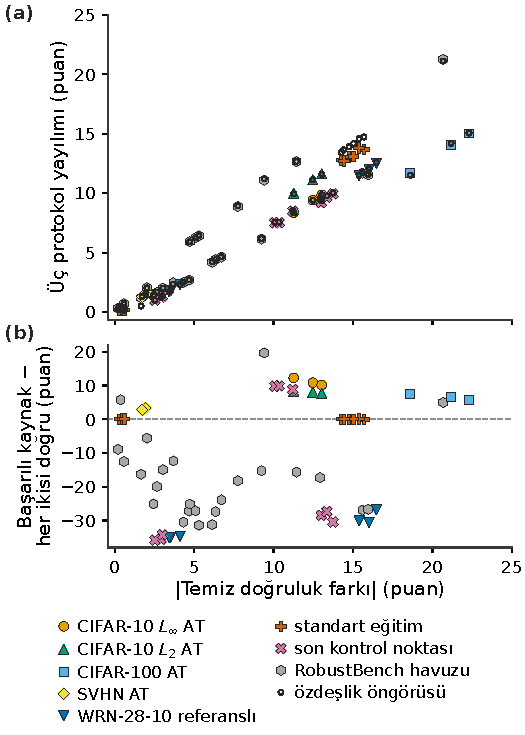
\includegraphics[width=\columnwidth]{../figures/final_tr/fig_spread_clean_gap.pdf}
\caption{Ölçülen $60$ model çiftinin tamamında protokol yayılımının mutlak temiz doğruluk farkına göre değişimi. (a) Asimetrinin koşulsuz, hedef doğru ve her ikisi doğru protokolleri üzerindeki yayılımı; küçük içi boş halkalar aynı çift için $p=1$ alınarak hesaplanan Denklem~\eqref{eq:raw_identity} öngörüsünü gösterir. (b) Aynı çiftlerde başarılı kaynak eksi her ikisi doğru asimetrisi, yani üç protokollü yayılımın dışarıda bıraktığı terim. İşaretçiler her ayarın çekişmeli eğitilmiş çiftlerini, bunların WideResNet-28-10 referansıyla eşleşmelerini, son kontrol noktasındaki aynı çiftleri, standart eğitilmiş çiftleri ve RobustBench havuzunu ayırır; çiftler modelleri paylaştığı için uydurma doğrusu çizilmemiştir.}
\label{fig:spread_clean_gap}
\end{figure}

% REF: Yayilim - temiz fark iliskisi (tum ciftler): uc protokol egim +0.796, r 0.9571, grup-birak +0.767; +0.855;
%      57/60 esitlik; ozdeslik paritesi en buyuk 1.09, ortalama 0.13; dort protokol +0.092, r 0.0532
Şekil~\ref{fig:spread_clean_gap} ilişkiyi ölçülen her çifte genişletmektedir. Bu çiftler üç veri kümesinin ve iki tehdit modelinin çekişmeli eğitilmiş çiftleri, bunların WideResNet ile eşleşmeleri, son kontrol noktasındaki aynı CIFAR-10 çiftleri (Bölüm~\ref{subsec:selection}), standart eğitilmiş çiftler ve Bölüm~\ref{subsec:external}'teki dış havuzdur; toplam $60$ sırasız çift söz konusudur. CIFAR-100 ve $L_2$ ayarlarının WideResNet eşleşmeleri dahil edilmemiş, havuzun ilk CIFAR-10 eğitim çiftiyle çakışan üç çifti ise çekişmeli eğitilmiş gruplarda bir kez sayılmıştır. Üç protokollü yayılım farkla birlikte artmakta (eğim $+0{,}796$, Pearson $r = 0{,}957$; herhangi bir grup dışarıda bırakıldığında $+0{,}767$ ile $+0{,}855$ arasında) ve $60$ noktanın $57$'sinde koşulsuz eksi hedef doğru farkına eşit olmaktadır. İçi boş halkalarla çizilen Denklem~\eqref{eq:raw_identity} öngörüsü her noktayı $1{,}09$ puan içinde izlemekte (ortalama mutlak sapma $0{,}13$), en büyük sapmalar ise $p$'nin birden en uzak olduğu standart eğitilmiş hedeflerde görülmektedir (Bölüm~\ref{subsec:external}). Dört protokollü yayılım farkı izlememekte (eğim $+0{,}092$, $r = 0{,}053$) ve temiz doğrulukları neredeyse eşit gürbüz çiftlerde büyük kalmaktadır. Bu yayılım Carmon vd.~\cite{carmon2019unlabeled} ile Gowal vd.'nin~\cite{gowal2020uncovering} iki WideResNet-28-10 kontrol noktasında ($0{,}21$ puan fark) $9{,}03$, XCiT-S12 ile Gowal vd.\ modelinde ($0{,}58$) $12{,}73$, bu çalışmanın ResNet-18 modeli ile Engstrom vd.'nin~\cite{engstrom2019robustness} ResNet-50 modelinde ($1{,}66$) ise $17{,}50$ puandır. Bunun nedenini (b) paneli göstermektedir. Başarılı kaynak terimi farkla ilişkisizdir; PGD-10 gürbüz doğrulukları sıfıra yakın olduğu için hemen her kaynak saldırısının başarılı olduğu standart eğitilmiş çiftlerde sıfıra yakın, gürbüz modeller arasında ise büyüktür ve iki işaretten birini taşımaktadır. Çiftler modelleri ve koşumları paylaştığı için bu eğimler havuzu betimlemekte, hiçbir şeyi sınamamaktadır.

% REF: Yayilim - temiz fark iliskisi, grup araliklari (SVHN uc protokol 1.30; 1.49)
% REF: Standart egitimli hedeflerde oncul p, cift turune gore ozet (0.47+-0.16; 0.19+-0.02)
Eşlenmiş çift öngörüsü ayrı bir bulgu değil, özdeşliğin bir sonucudur. Koşulsuz, hedef doğru ve her ikisi doğru kestirimleri temiz hatalarla ölçeklenen terimler üzerinden ayrıştığından, temiz doğrulukta eşlenmiş bir çiftin mimarisi ne olursa olsun bu kestirimleri birbirine yakın bırakması beklenir. Verilerin katkısı, öngörünün gerektirdiği üç ölçülmüş olgudur. İncelenen her çekişmeli eğitilmiş hedefte $p$ en az $0{,}984$'tür, her ikisi doğru kestirimi $60$ noktanın $57$'sinde diğer ikisinin arasında yer almaktadır ve başarılı kaynak terimi farka bağlı değildir. Buna uygun olarak $1{,}84$ puanlık farkla SVHN'in iki çiftinde üç protokollü yayılım $1{,}49$ ve $1{,}30$ puandır; aralarında $0{,}47\pm0{,}16$ puan bulunan standart eğitilmiş ResNet-18 ile WideResNet-28-10 çiftinde ise dört protokolün tamamı $0{,}19\pm0{,}02$ puan içindedir (Bölüm~\ref{subsec:external}). CIFAR-10'daki $15$ puanlık aralığın temiz doğruluk farkından gelen kısımları, yani özdeşlik terimi ve onaylanan ikili içindeki uzaklık, temiz doğrulukta eşlenmiş çiftlerde küçülmelidir; yukarıdaki gürbüz çiftlerin gösterdiği gibi başarılı kaynak fazlasının küçülmesi ise gerekmemektedir.

% ----------------------------------------------------------------------------
% E. Standart egitilmis hedefler ve dis havuz
% ----------------------------------------------------------------------------
\subsection{Standart Eğitilmiş Hedefler ve Dış Model Havuzu}
\label{subsec:external}

% REF: Standart egitimli hedeflerde oncul p (temiz ciftler); RobustBench havuzu (8 model, tohum 42)
\begin{sloppypar}
Bu çalışmanın çekişmeli eğitilmiş çiftinin yanıtlayamadığı iki soru kalmaktadır. Bunlar öncül $p$'nin transfer çalışmalarının çoğunun saldırdığı rejim olan standart eğitilmiş hedeflerde sağlanıp sağlanmadığı ve eşlenmiş çift öngörüsünün başkalarının eğittiği modellerde tutup tutmadığıdır. İki soru da yeni bir eğitim yapılmadan yanıtlanmıştır. İlk olarak üç eğitim çiftinin, çekişmeli ince ayarın başlangıç noktaları olan temiz eğitilmiş ResNet-18 ve ViT-Tiny kontrol noktaları, RobustBench~\cite{croce2021robustbench} üzerinden dağıtılan standart eğitilmiş WideResNet-28-10 (tanımlayıcı \texttt{Standard}) ile birleştirilerek çift başına bir $3\times3$ matris kurulmuştur. İkinci olarak sekiz modelli bir CIFAR-10 havuzu, ilk çiftin çekişmeli eğitilmiş ResNet-18 ve ViT-Tiny modellerini, standart eğitilmiş WideResNet'i ve RobustBench tanımlayıcılarıyla anılan beş gürbüz RobustBench kontrol noktasını bir araya getirmektedir: bir PreAct ResNet-18 (\texttt{Wong2020Fast})~\cite{wong2020fast}, bir ResNet-50 (\texttt{Engstrom2019Robustness})~\cite{engstrom2019robustness}, etiketsiz veriyle eğitilmiş bir WideResNet-28-10 (\texttt{Carmon2019Unlabeled})~\cite{carmon2019unlabeled}, dikkati evrişim bileşenleriyle birleştiren bir XCiT-S12 (\texttt{Debenedetti2022Light\_XCiT-S12})~\cite{debenedetti2023light} ve önceki bölümlerin WideResNet-28-10 referansı~\cite{gowal2020uncovering}. Her yöne tam test kümesinde, örnek bazında kayıtla $\eps=8/255$ bütçeli PGD-10 saldırısı uygulanmış; dört protokol, $p$ ve $p=1$ artığı bu kayıtlardan hesaplanmıştır (Tablo~\ref{tab:external_pool}).
\end{sloppypar}

% REF: Standart egitimli hedeflerde oncul p, hedef turune gore (tum yonler 0.8774-1.0000; Standard WRN hedef 0.8774-0.9962;
%      ViT temiz hedef 0.9231-0.9338; artik en buyuk 1.58)
% REF: RobustBench havuzu (56 yon, p 0.9330-1.0000; artik en buyuk 0.35; AT hedeflerde p en kucuk 0.9846)
% REF: Secim kuralinin asimetriye etkisi, B (son kontrol noktasi p en kucuk 0.9915; artik en buyuk 0.20)
Standart eğitilmiş hedeflerde öncül zayıflamaktadır. Üç temiz matrisin $18$ köşegen dışı yönünde $p$ değeri $0{,}877$ ile $1{,}000$ arasında değişmektedir; en düşük değerler standart eğitilmiş WideResNet hedef olduğunda görülmekte ($0{,}877$ ile $0{,}996$), temiz ViT-Tiny hedefinde ise $p$ $0{,}923$ ile $0{,}934$ arasında kalmaktadır. Bu durumda $p=1$ biçimi koşulsuz oranı, üç hedef içinde temiz hatası en büyük olan ViT-Tiny hedefinde $1{,}58$ puana kadar ıskalamaktadır. Orada Denklem~\eqref{eq:raw_identity} bir üst sınırdır ve kullanılması gereken düzeltme, ölçülmüş $p$ ile genel biçim olan Denklem~\eqref{eq:general_identity}'dir. Sekiz hedeften yedisinin çekişmeli eğitilmiş olduğu havuzda her çekişmeli eğitilmiş hedefte $p\geq0{,}984$, standart eğitilmiş hedefte $p\geq0{,}933$'tür ve $p=1$ artığı $56$ yönün tamamında $0{,}35$ puan içinde kalmaktadır; bu çalışmanın çiftlerinin son kontrol noktasında ise artık $0{,}20$ puanı aşmamaktadır (Bölüm~\ref{subsec:selection}).

% REF: Standart egitimli hedeflerde oncul p, cift basina dort protokol asimetrisi ve cift turune gore ozet
Standart eğitilmiş matrisler eşlenmiş çift öngörüsünü farklı bir eğitim rejiminde de sınamaktadır. Temiz ResNet-18 ile standart WideResNet temiz doğrulukta $0{,}47\pm0{,}16$ puan ayrışmakta ve dört protokol kestirimleri $0{,}19\pm0{,}02$ puan içinde uyuşmaktadır (ilk çiftte $-3{,}35$, $-3{,}54$, $-3{,}51$ ve $-3{,}50$). Yaklaşık $15$ puan ayrışan iki eşlenmemiş çiftte ($15{,}16\pm0{,}48$ ve $14{,}69\pm0{,}60$) yayılım $13{,}25\pm0{,}34$ ve $13{,}08\pm0{,}60$ puandır ve her koşuda koşulsuz protokol diğer üçünün bildirdiği işareti tersine çevirmektedir; temiz ResNet-18 ve ViT-Tiny için koşulsuz protokol $+7{,}81$ ile $+10{,}09$ puan verirken hedef doğru protokolü $-5{,}22$ ile $-3{,}56$ puan vermektedir. Dolayısıyla standart eğitim altında bu çalışmanın ResNet-18 ve ViT-Tiny modelleri her koşullu protokolde ters yönü, yani Mahmood vd.'nin bildirdiği yönü göstermektedir (her ikisi doğru $-3{,}02$ ile $-1{,}30$), ancak onların mekanizmasını göstermemektedir. Toplamsal uydurma (Tablo~\ref{tab:source_target}) temiz ViT-Tiny modelini açık ara en zayıf kaynak olarak tutmakta (kaynak farkı $+69{,}18\pm2{,}31$) ve işareti hedef terimi üzerinden çevirmektedir ($-75{,}05\pm1{,}72$); temiz ViT-Tiny, zayıf bir kaynak olduğundan da daha zor bir hedeftir. Standart WideResNet iki karşıtlığı da doğrudan göstermektedir; ResNet'te üretilen örneklerin $\%81{,}40$'ı, ViT'te üretilenlerin ise $\%13{,}60$'ı tarafından kandırılmakta, kendisi de ResNet'i $\%84{,}05$, ViT'i $\%7{,}62$ oranında kandırmaktadır.

% REF: RobustBench havuzu (28 cift; temiz fark 0.21-20.68; uc protokol +0.872 [+0.534; +1.274], r 0.9438;
%      dort protokol +0.559 [-0.205; +4.582]; isaret donen 1/28; ViT_Tiny_AT/Standard -6.72 / +14.53, fark 20.68;
%      Carmon2019/Gowal2020: fark 0.21, uc 0.32, dort 9.03; toplamsal: R2 0.8955, kaynak etkileri, hedef etkileri)
Temiz farkları $0{,}21$ ile $20{,}68$ puan arasında değişen $28$ çiftli havuzda üç protokollü yayılım temiz farkın puanı başına $0{,}872$ puan artmakta (model dışarıda bırakmalı bootstrap aralığı $[+0{,}534;\ +1{,}274]$, $r = 0{,}944$), dört protokollü yayılım ise güvenilir bir ilişki göstermemektedir ($+0{,}559$, $[-0{,}205;\ +4{,}582]$). İşaret protokoller arasında $28$ çiftin yalnızca birinde, bu çalışmanın çekişmeli eğitilmiş ViT-Tiny modeli ile standart eğitilmiş WideResNet çiftinde değişmektedir; bu çift aynı zamanda en geniş farka sahip çifttir ($20{,}68$ puan; koşulsuz $-6{,}72$, hedef doğru $+14{,}53$). Temiz doğrulukları neredeyse eşit gürbüz modeller eşlenmiş çift öngörüsünü ve onun sınırını aynı anda doğrulamaktadır. Carmon vd.\ ile Gowal vd.'nin aralarında $0{,}21$ puan bulunan iki gürbüz WideResNet-28-10 kontrol noktasında üç protokollü yayılım $0{,}32$, dört protokollü yayılım ise $9{,}03$ puandır. Havuzun hedef doğru matrisine yapılan toplamsal uydurma ($56$ hücrede $R^2 = 0{,}8955$) bu çalışmanın ViT-Tiny modelini çekişmeli eğitilmiş en zayıf kaynak olarak konumlandırmakta (kaynak etkisi $-4{,}87$, diğer gürbüz modellerde $+2{,}94$ ile $+3{,}65$), hedef etkisini ise gürbüz modellerin aralığı ($-4{,}26$ ile $+2{,}76$) içinde $-0{,}63$ olarak vermektedir. Evrişim bileşenli bir dikkat modeli olan gürbüz XCiT-S12, CNN'ler kadar güçlü bir kaynaktır ($+3{,}06$). Bölüm~\ref{subsec:source_target}'deki kaynak etkisi bu nedenle bir aile olarak dönüştürücülerin değil, sıfırdan düşük bir temiz doğruluğa eğitilmiş bu ViT-Tiny modelinin özelliği olarak okunmalıdır; havuzdaki tek gürbüz dikkat tabanlı model daha fazlasını söylemeye yetmemektedir.

% REF: tablo hucreleri: "Standart egitimli hedeflerde oncul p", "RobustBench havuzu",
%      "Secim kuralinin asimetriye etkisi" B, ozdeslik_kontrol.json (36 yon, 0.41)
\begin{table}[!t]
\centering
\caption{Denklem~\eqref{eq:general_identity}'deki öncül $p$ ve bu çalışmanın çekişmeli eğitilmiş çifti dışında eşlenmiş çift öngörüsü (CIFAR-10, PGD-10, $\eps$=8/255, tam test kümesi). Üst blok: köşegen dışı yönler üzerinden hedef türüne göre $p$ ve $p=1$ biçiminin puan cinsinden en büyük mutlak hatası (``--'': hedef türü başına saklanmamıştır). Orta blok: her biri bir eğitim çiftinin temiz ResNet-18 ya da ViT-Tiny modeli veya RobustBench'in standart eğitilmiş WideResNet-28-10 modeli olan standart eğitilmiş çiftler, üç çift üzerinden ortalama$\pm$std; işaret dönmesi dört protokolün işarette uyuşmadığını gösterir. Alt blok: sekiz modelli havuzun $28$ çifti üzerinde protokol yayılımının mutlak temiz doğruluk farkına göre eğimi; çiftler modelleri paylaştığı için aralık model dışarıda bırakmalı bootstrap ile verilmiştir.}
\label{tab:external_pool}
\footnotesize
\setlength{\tabcolsep}{3pt}
\begin{tabular}{lccc}
\toprule
\textbf{Hedef} & \textbf{Yön} & \textbf{$p$ aralığı} & \textbf{Maks.\ $|$artık$|$} \\
\midrule
AT hedefleri, $3\times3$ & 36 & 0,9890--1,0000 & 0,41 \\
AT hedefleri, son k.\,n. & 18 & 0,9915--1,0000 & 0,20 \\
Temiz ViT-Tiny & 6 & 0,9231--0,9338 & 1,58 \\
Temiz ResNet-18 & 6 & 0,8961--1,0000 & 0,51 \\
Standart WRN-28-10 & 6 & 0,8774--0,9962 & 0,64 \\
Havuz, AT hedefleri & 49 & 0,9846--1,0000 & -- \\
Havuz, standart WRN & 7 & 0,9330--0,9962 & -- \\
Havuz, tüm hedefler & 56 & 0,9330--1,0000 & 0,35 \\
\midrule
\textbf{Std.\ eğitilmiş çift} & \textbf{$|$Temiz fark$|$} & \textbf{Yayılım} & \textbf{İşaret dön.} \\
\midrule
ResNet-18 / WRN & 0,47$\pm$0,16 & 0,19$\pm$0,02 & 0/3 \\
ResNet-18 / ViT-Tiny & 15,16$\pm$0,48 & 13,25$\pm$0,34 & 3/3 \\
ViT-Tiny / WRN & 14,69$\pm$0,60 & 13,08$\pm$0,60 & 3/3 \\
\midrule
\textbf{Havuz yayılımı} & \textbf{Eğim} & \textbf{\%95 aralık} & \textbf{$r$} \\
\midrule
Üç protokol & $+$0,872 & [$+$0,534; $+$1,274] & 0,944 \\
Dört protokol & $+$0,559 & [$-$0,205; $+$4,582] & 0,350 \\
İşaret dön.\ (4 prot.) & \multicolumn{3}{c}{1/28 çift} \\
\bottomrule
\end{tabular}
\end{table}

% ----------------------------------------------------------------------------
% F. Kontrol noktasi secimi
% ----------------------------------------------------------------------------
\subsection{Kontrol Noktası Seçimi ve Asimetri}
\label{subsec:selection}

Sabit bir yörüngeden son kontrol noktasını seçen çevrimdışı kural, gürbüz aşırı öğrenme bu seçimi çekişmeli eğitimde sonuç doğurucu kılsa da~\cite{rice2020overfitting} genellikle örtük bırakılmaktadır. Bir eğitim yörüngesi sabit tutulup yalnızca son kontrol noktasının nasıl seçildiği, yani doğrulama bölmesi, erken durdurma sabrı ve argmaks öncesinde doğrulama eğrisinin yumuşatılıp yumuşatılmadığı değiştirildiğinde (on sekiz bileşim) raporlanan PGD-10 doğruluğu ResNet'te tohum başına $2{,}62$ ile $2{,}85$, ViT'te $1{,}58$ ile $2{,}09$ puan oynamaktadır. Bu hücrelerde diskteki ağırlıklar özdeştir ve yalnızca içlerinden birini seçen kural farklıdır. Bu yayılımın yaklaşık yarısı üç boyuttan yalnızca birinden gelmektedir. Argmaks öncesinde doğrulama eğrisini yumuşatmak, üç ResNet koşumunun üçünde ve üç ViT koşumunun ikisinde test PGD-10 doğruluğunu monoton biçimde düşürmektedir; yani sistematik olarak daha kötü bir kuraldır. Çalışmaların fiilen değiştirdiği bölme ve sabır seçimleriyle sınırlandığında yayılım ResNet'te tohum düzeyi standart sapmanın $1{,}09$ katına, ViT'te $1{,}42$ katına inmektedir. Bu yayılım mutlak birimlerle raporlanmakta ve bilinçli olarak tohum düzeyi yayılıma oran biçiminde verilmemektedir; çünkü o oran on sekiz hücreden hangisinin referans alındığına bağlıdır ve on sekizinin tamamı tarandığında ResNet'te $0{,}67$ ile $3{,}38$, ViT'te $0{,}63$ ile $7{,}38$ arasında değişerek bazı referanslarda karşılaştırmayı tersine çevirmektedir.

CIFAR-100 koşuları bir karşı ağırlık sağlamaktadır. Bu çalışmanın protokolünün seçtiği epok üç ResNet tohumu arasında $25$ epok kaymakta, buna karşılık ortaya çıkan test PGD-10 standart sapması $0{,}32$ puanda kalmaktadır. Seçim \emph{yolu} oynak, seçilen \emph{sonuç} ise kararlı olmuştur; bunlardan hangisinin gerçekleşeceği mimariye değil yörüngenin platosuna bağlıdır.

% REF: Secim kuralinin asimetriye etkisi, B. Son kontrol noktasi ve fark ozeti
%      (temiz fark 12.26+-0.90 -> 10.55+-0.59, degisim -1.71+-0.84; dort yayilim 15.01+-0.84 -> 12.84+-0.34,
%       degisim -2.16+-0.93; uc yayilim 9.21+-0.76 -> 7.84+-0.56; tc +4.36+-0.44 -> +4.64+-0.56;
%       ss +19.37 -> +17.48; p en kucuk 0.9915; artik en buyuk 0.20)
Seçim kuralı, yayılımın bağlı olduğu temiz doğruluk farkını belirlediği için transfer asimetrisine de ulaşmaktadır. Üç eğitim çiftinin seçilen kontrol noktası yerine son kontrol noktasında, yani erken durdurmanın eğitimi sonlandırdığı epokta yeniden puanlanması (ResNet'ler için $71$, $76$ ve $77$, ViT'ler için $45$, $38$ ve $39$; seçilen $51$, $56$, $57$ ve $25$, $18$, $19$. epoklardan yirmi epok sonra) temiz farkı $12{,}26\pm0{,}90$ puandan $10{,}55\pm0{,}59$ puana (değişim $-1{,}71\pm0{,}84$), dört protokollü yayılımı ise $15{,}01\pm0{,}84$ puandan $12{,}84\pm0{,}34$ puana (değişim $-2{,}16\pm0{,}93$) daraltmaktadır; üç protokollü yayılım da $9{,}21\pm0{,}76$'dan $7{,}84\pm0{,}56$'ya inmektedir. Hedef doğru asimetrisi neredeyse yerinden oynamamakta ($+4{,}36\pm0{,}44$'e karşı $+4{,}64\pm0{,}56$), başarılı kaynak kestirimi $+19{,}37$'den $+17{,}48$'e düşmekte, dört protokolün tamamı her çiftte CNN$\rightarrow$ViT işaretini korumakta ve öncül önceki gibi sağlanmaktadır ($p\geq0{,}9915$, $p=1$ artığı en çok $0{,}20$ puan).

% REF: Secim kuralinin asimetriye etkisi, A. Saklanan egitim yorungeleri (CIFAR-10 temiz fark secilen 10.59-12.65,
%      son 11.83-13.83; yayilim Delta ResNet -1.53+-1.15, ViT -0.03+-1.15; tc Delta ViT +2.53+-0.15;
%      CIFAR-100 yayilim Delta ResNet -1.84+-0.94, ViT +0.84+-0.24)
Saklanan eğitim yörüngeleri eğitim boyunca aynı tabloyu vermektedir. Bu yörüngeler ana çiftlerin seçilen kontrol noktalarından değil, aynı tohumlarla yapılan CIFAR-10 yeniden eğitim koşularından ve doğrudan CIFAR-100 koşularından gelmekte ve yaklaşık her on epokta bir kaydedilmektedir. CIFAR-10'da bu yeniden eğitim koşuları temiz farkı hem seçilen hem son epokta $10{,}59$ puanda ya da üstünde tutmaktadır; dolayısıyla seçim farkı yaklaşık $1{,}7$ puan oynatmakta, ancak ortadan kaldırmamaktadır. Farkın tam büyüklüğü ise seçime duyarlıdır. Bir çiftin bir üyesini seçilen epoğundan son epoğuna taşımak dört protokollü yayılımı ResNet taşındığında $-1{,}53\pm1{,}15$ puan, ViT taşındığında $-0{,}03\pm1{,}15$ puan değiştirmekte, ViT'in taşınması ise hedef doğru asimetrisini $+2{,}53\pm0{,}15$ puan kaydırmaktadır; CIFAR-100'de yayılım $-1{,}84\pm0{,}94$ ve $+0{,}84\pm0{,}24$ puan değişmektedir. Seçim kuralı böylece asimetrinin düzeyini yaklaşık iki buçuk puana, yayılımını ise yaklaşık iki puana kadar oynatmakta, ancak yönü ya da büyüklük mertebesini değiştirmemektedir. Bu kuralın yöntem bölümünde belirtilmesi gerekir.

% ----------------------------------------------------------------------------
% G. Uc okuma (gradyan, dikkat, TGR tek alt bolumde)
% ----------------------------------------------------------------------------
\subsection{Doğrudan Ölçümde Ayakta Kalmayan Üç Okuma}
\label{subsec:readings}

Mimari karşılaştırmaları transfer asimetrisinin ötesinde üç okumayı da akla getirmektedir: CNN gradyanlarının mekansal olarak daha lokalize olduğu, çekişmeli pertürbasyonun ViT dikkatini bozduğu ve ViT'e özgü transfer saldırılarının ViT kaynaklı transferi iyileştirdiği. Her biri doğrudan ölçülmüş, hiçbiri bu rejimde geçerli çıkmamış ve aynı ölçümler iki davranışsal farkı ayakta bırakmıştır.

% ----------------------------------------------------------------------------
% G.1 Gradyan seyrekligi ve mekansal lokalite
% ----------------------------------------------------------------------------
\subsubsection{Mekansal lokalite olmadan gradyan seyrekliği}
\label{subsec:gradient}
\label{subsubsec:spatial}

\begin{table}[!t]
\centering
\caption{Örnek başına kayıp gradyanlarından hesaplanan gradyan karakteristikleri (koşu başına $n$=500 test örneği; üç koşu üzerinden ortalama$\pm$std). Kalın yazı, çekişmeli eğitilmiş iki modelden büyük olanı gösterir; yerel kontrol tek bir kontrol noktası olduğundan standart sapma verilmemiştir.}
\label{tab:gradient}
\footnotesize
\setlength{\tabcolsep}{2.5pt}
\begin{tabular}{lccc}
\toprule
\textbf{Metrik} & \textbf{ResNet-18 AT} & \textbf{ViT-Tiny AT} & \textbf{ViT (yerel)$^\ddagger$} \\
\midrule
Hoyer seyrekliği & \textbf{0,4928}$\pm$0,0120 & 0,4561$\pm$0,0055 & 0,4046 \\
Gini katsayısı & \textbf{0,6498}$\pm$0,0089 & 0,6099$\pm$0,0051 & 0,5712 \\
Maks.\ \%1 altı kesir & \textbf{0,3477}$\pm$0,0210 & 0,2682$\pm$0,0090 & 0,1785 \\
Hizalanma (mutlak) & 0,0378$\pm$0,0009 & \textbf{0,0562}$\pm$0,0004 & 0,0794 \\
Hizalanma (işaretli) & 0,0010$\pm$0,0003 & 0,0004$\pm$0,0001 & -- \\
\bottomrule
\multicolumn{4}{l}{\scriptsize $^\ddagger$CIFAR'a özgü ViT kontrolü ($4\times4$ yama, 5,4M parametre); sabit bölme}\\
\multicolumn{4}{l}{\scriptsize \phantom{$^\ddagger$}protokolünden önceye ait, test kümesinde seçilmiş tek kontrol noktası;}\\
\multicolumn{4}{l}{\scriptsize \phantom{$^\ddagger$}yalnızca büyütme etkisinin işareti için eklenmiştir.}
\end{tabular}
\end{table}

% REF: Gradyan yapisi (Hoyer temiz 0.3467 / 0.3804; hizalanma temiz 0.0293 / 0.0581; Cohen d 0.32-1.23; isaretli en buyuk 0.0014)
CNN girdi gradyanları üç ölçekten bağımsız ölçünün üçünde de ViT gradyanlarından daha seyrektir (Tablo~\ref{tab:gradient}; normlar değerlendirme parti boyuna bağlı olmasın diye örnek başına kayıp gradyanları, hizalanma için tüm $500\times499/2$ örnek çifti üzerinden ortalama mutlak kosinüs) ve sıralama, tohum düzeyi standart sapmalar farktan en az üç kat küçük kalarak her koşuda yeniden üretilmektedir. İki çıkarım biriminin uyuşmadığı tek yer burasıdır ve bu nedenle ikisi de raporlanmaktadır. Aynı 500 örneğin iki modelde de ölçüldüğü koşum içinde örnek başına eşleştirilmiş Wilcoxon testleri üç ölçüde de sıfır hipotezini reddetmektedir (Holm düzeltmeli $p<10^{-11}$, eşleştirilmiş Cohen $d$ 0,32 ile 1,23 arasında). Mimari bir iddianın gerektirdiği birim olan koşum düzeyinde ise üç eşleştirilmiş koşum Gini, \%1 altı kesir ve Hoyer için $0{,}036$, $0{,}042$ ve $0{,}067$ ham $p$ değerleri vermekte, Holm düzeltmesi bunları $0{,}108$'e çıkarmaktadır. Sıralama her koşuda tutarlı ama koşum düzeyinde anlamsız olduğu için anlamlı olarak değil, yeniden üretilebilir olarak raporlanmaktadır. Sıralama çekişmeli eğitimin ürünüdür. Aynı koşuların temiz eğitilmiş karşılıklarında daha seyrek model \emph{ViT'tir} (Hoyer $0{,}380\pm0{,}009$'a karşı $0{,}347\pm0{,}002$); bu durum Chalasani vd.'nin~\cite{chalasani2020concise} çekişmeli eğitilmiş modeller için bildirdiği daha seyrek öznitelik atıflarıyla uyumludur. CIFAR'a özgü ViT kontrolü ise her ölçüde büyütülmüş ViT'ten daha az seyrektir; dolayısıyla sıralama $32\rightarrow224$ büyütmenin artefaktı değildir. Örnekler arası hizalanma mutlak kosinüste ViT'te daha yüksektir; bu fark koşum düzeyinde anlamlılığa ulaşmakta ($p=0{,}0009$) ve temiz eğitilmiş çiftte zaten görülmektedir ($0{,}058$'e karşı $0{,}029$). \emph{İşaretli} ortalama kosinüs ise iki modelde de sıfıra yakındır (her koşumda $\leq0{,}0014$); yani örnekler duyarlılık eksenlerini paylaşmakta, ancak tutarlı bir yönü paylaşmamaktadır.

\begin{table}[!t]
\centering
\caption{Girdi gradyanlarının mekansal lokalitesi (koşu başına $n$=500 örnek; üç koşu üzerinden ortalama$\pm$std). Eşleştirilmiş farklar aynı örnekler üzerinde hesaplanır. Çıkarım koşum düzeyindedir: $p$, üç koşumun ortalama farkları üzerinde tek örneklem $t$ testidir ve dört ölçüye Holm düzeltmesi uygulanmıştır; böylece çıkarımın birimi iddianın birimiyle eşleşir. Düşük alan ve entropi daha lokalize, yüksek Moran's $I$ daha kümeli demektir.}
\label{tab:spatial}
\scriptsize
\setlength{\tabcolsep}{1.6pt}
\begin{tabular}{lcccc}
\toprule
\textbf{Ölçüt} & \textbf{ResNet-18} & \textbf{ViT-Tiny} & \textbf{Fark (R$-$V)} & \textbf{$p$ (Holm)} \\
\midrule
\%50 enerji alanı & 0,0378$\pm$0,0017 & 0,0397$\pm$0,0010 & $-$0,0019$\pm$0,0027 & 0,54 \\
\%90 enerji alanı & 0,2345$\pm$0,0078 & 0,2570$\pm$0,0067 & $-$0,0224$\pm$0,0133 & 0,40 \\
Mekansal entropi (nat) & 5,2014$\pm$0,0387 & 5,2524$\pm$0,0197 & $-$0,0509$\pm$0,0580 & 0,54 \\
Moran's $I$ & 0,4141$\pm$0,0132 & 0,3941$\pm$0,0024 & $+$0,0200$\pm$0,0156 & 0,47 \\
\bottomrule
\end{tabular}
\end{table}

% REF: Tablo 9 ek sutunlari (Holm p 0.402-0.535; kosum degerleri: alan50 ve entropi isaret degistiriyor)
Seyreklik kaç gradyan bileşeninin büyük olduğunu saymakta, ancak bu bileşenlerin görüntüde bir arada durup durmadığını, yani gradyanları lokalize olarak betimleyen ifadenin ileri sürdüğü şeyi söylememektedir. Aynı gradyanların kanal toplamı enerji haritası üzerinde dört ölçekten bağımsız betimleyicinin hiçbiri koşum düzeyinde farklılaşmamaktadır (Tablo~\ref{tab:spatial}; Holm düzeltmeli $p$ değerleri $0{,}40$ ile $0{,}54$ arasında). Enerjinin \%90'ını taşıyan alan CNN için görüntü alanının iki yüzde puanı kadar \emph{daha küçük} bir alana işaret etmekte ve dört mekansal sıralamanın ikisi koşumlar arasında işaret değiştirmektedir; seyreklik sıralaması ise her koşuda her ölçüde korunmaktadır. Çekişmeli eğitilmiş CNN gradyanları kütlelerinin daha büyük kısmını daha az piksele yerleştirmekte, ancak bu pikseller ViT'inkilerden mekansal olarak daha kümeli olmamaktadır; bu nedenle bu çalışmanın iddiaları seyreklikle sınırlı tutulmuştur. Şekil~\ref{fig:gradient_analysis} ölçekten bağımsız ölçülerin yakalamadığı örnek başına gradyan normlarının dağılımını eklemektedir; Şekil~\ref{fig:gradient_heatmap}'teki büyüklük haritaları da lokalite olarak değil seyreklik olarak okunmalıdır.

\begin{figure}[!t]
\centering
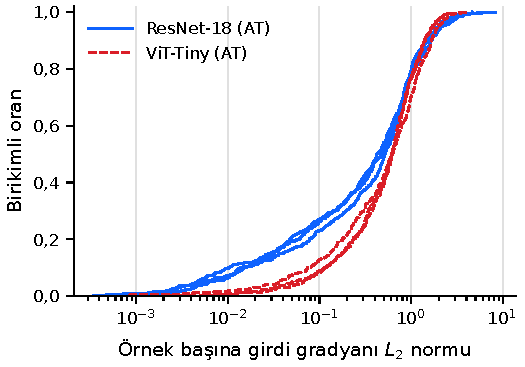
\includegraphics[width=\columnwidth]{../figures/final_tr/fig4b_gradient_distribution.pdf}
\caption{Örnek başına girdi gradyanı $L_2$ normlarının deneysel dağılımı (örnek başına çapraz entropi kaybı, ilk $500$ test görüntüsü, eğitim koşusu başına bir eğri, mimari başına üç koşu; logaritmik eksen). Bu girdilerden dördünün büyüklük haritaları Şekil~\ref{fig:gradient_heatmap}'te verilmektedir.}
\label{fig:gradient_analysis}
\end{figure}

\begin{figure}[!t]
\centering
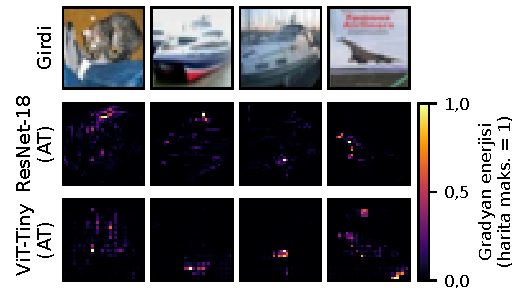
\includegraphics[width=\columnwidth]{../figures/final_tr/fig4_gradient_comparison.pdf}
\caption{Aynı test görüntüleri için iki modelde girdi gradyanı büyüklük haritaları (tohum çifti 1; ilk dört test görüntüsü; her harita kendi en büyük değerine ölçeklendiğinden büyüklükler paneller arasında karşılaştırılamaz). CNN gradyanları kütlelerinin daha büyük kısmını daha az bileşene yerleştirmektedir (Tablo~\ref{tab:gradient}). Tablo~\ref{tab:spatial} bu durumun mekansal dizilişte bir farkla birlikte gelmediğini göstermektedir; bu yüzden paneller lokalite olarak değil seyreklik olarak okunmalıdır.}
\label{fig:gradient_heatmap}
\end{figure}

% ----------------------------------------------------------------------------
% G.2 Dikkat ve oznitelik kaymasi
% ----------------------------------------------------------------------------
\subsubsection{Dikkat entropisi ve öznitelik kayması}
\label{subsec:attention}

\begin{table}[!t]
\centering
\caption{Her modelin kendi beyaz kutu PGD-10 saldırısı altında blok bazlı temizden çekişmeliye kosinüs benzerliği (koşu başına $n$=1000; üç koşu ortalaması). Tüm özetler artık blok çıkışında alınmıştır, böylece ViT ve CNN sütunları eşdeğer noktalarda ölçülmektedir; ViT sütunları yalnızca bir bloğun jetonlarının nasıl toplandığında ayrışır. MLP alt-blok çıkışına ait değerler metinde verilmiştir. Koşumlar arası standart sapma ViT sütunlarında en çok 0,0061, ResNet sütununda en çok 0,0181'dir (aşama 4, blok 1); kalın yazı her sütunun en küçük değerini gösterir.}
\label{tab:feature_degradation}
\footnotesize
\setlength{\tabcolsep}{2.5pt}
\begin{tabular}{lccc@{\hspace{9pt}}lc}
\toprule
\multicolumn{4}{c}{\textbf{ViT-Tiny AT}} & \multicolumn{2}{c}{\textbf{ResNet-18 AT}} \\
\cmidrule(lr){1-4} \cmidrule(lr){5-6}
\textbf{Blok} & \textbf{CLS} & \textbf{Yama ort.} & \textbf{Tüm jetonlar} & \textbf{Aşama.blok} & \textbf{Kosinüs} \\
\midrule
1 & 0,9993 & 0,9980 & 0,9927 & 1.1 & 0,9951 \\
2 & 0,9950 & 0,9959 & 0,9901 & 1.2 & 0,9918 \\
3 & 0,9902 & 0,9940 & 0,9881 & 2.1 & 0,9879 \\
4 & 0,9873 & 0,9919 & 0,9861 & 2.2 & 0,9853 \\
5 & 0,9845 & 0,9904 & 0,9847 & 3.1 & 0,9753 \\
6 & 0,9814 & 0,9894 & 0,9835 & 3.2 & 0,9607 \\
7 & 0,9782 & 0,9885 & 0,9826 & 4.1 & \textbf{0,8777} \\
8 & 0,9743 & 0,9875 & 0,9816 & 4.2 & 0,9108 \\
9 & 0,9703 & \textbf{0,9870} & 0,9809 & & \\
10 & 0,9661 & 0,9872 & 0,9805 & & \\
11 & \textbf{0,9604} & 0,9874 & \textbf{0,9803} & & \\
12 & 0,9663 & 0,9915 & 0,9837 & & \\
\bottomrule
\end{tabular}
\end{table}

% REF: C4: oznitelik kaymasi ve attention (CLS 0.9604 blok 11; yama 0.9870 blok 9; oran 3.05;
%      MLP alt-blok: CLS 0.9343 blok 10, yama 0.9840 blok 8); ResNet layer4.0 0.8777+-0.0181, -13.14+-1.89%; layer4.1 0.9108+-0.0060
Çekişmeli hasarın derinlik boyunca nerede biriktiği iki mimaride farklıdır (Tablo~\ref{tab:feature_degradation}; artık blok çıkışları, koşu başına $n=1000$) ve bu ölçüm temiz eğitilmiş ViT'lerin katman bazlı analizlerini~\cite{raghu2021vision} çekişmeli eğitilmiş ortama taşımaktadır. ViT'te kayma kademelidir ve yalnızca yönü değiştirmektedir. Benzerlik 11. bloktaki minimuma kadar azalmakta ve çıkışta hafifçe toparlanmakta, öznitelik normları ise temiz değerlerinin \%0,45'i içinde kalmaktadır. CNN'de ise hasar yoğunlaşmıştır; son aşamanın ilk bloğu $-\%13{,}14\pm1{,}89$'luk bir norm daralmasıyla $0{,}8777\pm0{,}0181$'e düşmekte, son blok ise temsili kısmen onarmaktadır ($0{,}9108\pm0{,}0060$). Ölçülen ViT profili jeton agregasyonuna bağlıdır. Minimumlarında CLS yolu yama jetonu ortalamasının yaklaşık üç katı kaymakta ($0{,}9604$'e karşı $0{,}9870$; $1-\cos$ cinsinden oran $3{,}05$) ve minimumlar farklı derinliklerde (blok 11 ve 9) bulunmaktadır; artık blok çıkışı yerine MLP alt-blok çıkışında okunduğunda minimumlar blok 10'da $0{,}9343$'e ve blok 8'de $0{,}9840$'a kaymaktadır. Farklı makalelerden katman bazlı kayma eğrileri ancak hem agregasyon hem de tensör belirtildiğinde karşılaştırılabilir.

% REF: Dikkat entropisi TOST ve devrilen/devrilmeyen kosinus (12/12; en buyuk p 0.00611; en buyuk |degisim| 0.0045;
%      temiz entropi 4.613-5.105; devrilen/devrilmeyen ViT 0.9895/0.9877, p 0.2010; ResNet 0.9058/0.9143, p 0.0804)
% REF: Dikkat entropisi ve CLS dikkat yer degistirmesi (TV 0.0276 -> 0.0841)
Dikkat okuması bu ölçümlerde doğrulanmamaktadır. Çekişmeli pertürbasyon CLS dikkat dağılımının entropisini değiştirmemektedir. Katman başına en büyük ortalama değişim $0{,}0045$ nat iken temiz katman ortalamaları $4{,}61$ ile $5{,}11$ nat arasındadır; ölçünün ölçeğinden sabitlenen $\pm0{,}05$ nat marjıyla üç koşum üzerinden yapılan koşum düzeyi TOST, $12$ katmanın tamamında eşdeğerliği kabul etmekte ve en zayıf sonuç $p=0{,}006$ olmaktadır (Şekil~\ref{fig:feature_degradation}a). Derinlikle büyüyen şey dikkat haritasının yer değiştirmesidir; bu değer ilk katmanda $0{,}028$ toplam varyasyondan son katmanda $0{,}084$'e çıkmaktadır (panel b). Dolayısıyla saldırı dikkati hafifçe yeniden yönlendirmekte, ancak genişletmemekte ya da keskinleştirmemektedir. Şekil~\ref{fig:attention_layers}'teki tek örnekli haritalar yayılmayı değil yeniden yönlendirmeyi göstermektedir ve 8 örneklik daha önceki bir şekil kümesi bu ölçümün desteklemediği bir dikkat etkisi izlenimi vermişti. Öznitelik kayması devrilen ve devrilmeyen örnekleri de ayırmamaktadır; buradaki devrilmeyen grup, modelin temiz girdide zaten yanlış sınıflandırdığı örnekleri de içermektedir. Son blok kosinüsü ViT'te devrilen örneklerde $0{,}9895$, devrilmeyenlerde $0{,}9877$, CNN'de ise $0{,}9058$ ve $0{,}9143$'tür; iki fark da koşum düzeyinde anlamlı değildir (üç koşum üzerinden eşleştirilmiş $t$, $p=0{,}20$ ve $p=0{,}080$), ancak CNN farkı üç koşumun üçünde de aynı işareti taşımaktadır. Yama pertürbasyonları altındaki dikkat kayması etkileri~\cite{gu2022vision} ve dikkat mekanizmasının kendisine yönelik saldırılar~\cite{fu2022patchfool} farklı bir tehdit modeline aittir.

\begin{figure}[!t]
\centering
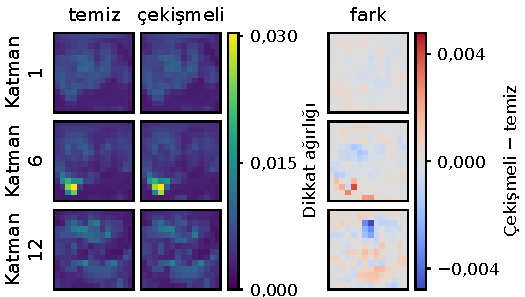
\includegraphics[width=\columnwidth]{../figures/final_tr/fig5_attention_comparison.pdf}
\caption{Çekişmeli saldırı altında ViT katmanları boyunca CLS jetonu dikkat haritaları (softmax sonrası, başlar üzerinden ortalanmış). Her satır farklı bir katmanı (1, 6, 12) gösterir; sütunlar temiz dikkat, çekişmeli dikkat ve farklarıdır ve dikkat sütunları için bir, fark sütunu için bir ortak renk ölçeği kullanılmıştır. Gösterilen tek bir örnektir (ilk test görüntüsü, tohum çifti 1); dikkat yer değiştirmesindeki derinlik eğilimi koşu başına $n$=1.000 örnek üzerinden Şekil~\ref{fig:feature_degradation}(b)'de ölçülmektedir.}
\label{fig:attention_layers}
\end{figure}

\begin{figure}[!t]
\centering
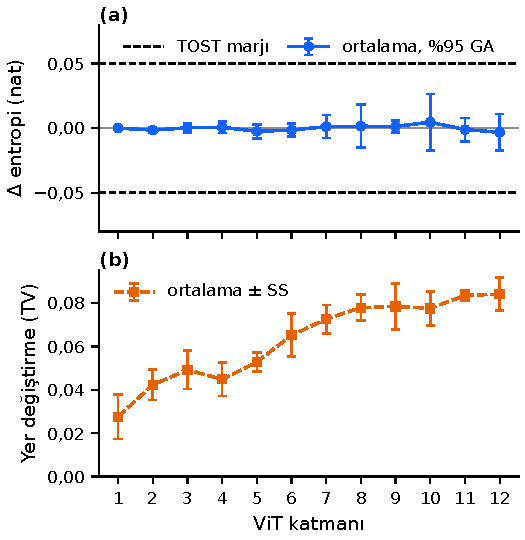
\includegraphics[width=\columnwidth]{../figures/final_tr/fig5b_attention_entropy.pdf}
\caption{(a) Saldırı altında CLS dikkat entropisindeki değişim (çekişmeli eksi temiz), katman başına, üç koşum ortalaması ve \%95 $t$ güven aralıkları; kesikli çizgiler $\pm0{,}05$ nat TOST marjını gösterir ve her aralık bu marjın içindedir. (b) CLS dikkat yer değiştirmesi (temiz ile çekişmeli haritalar arasındaki toplam varyasyon), katman başına, koşumlar üzerinden ortalama$\pm$std. Koşu başına $n$=1.000 örnek; tek örnekli haritalar Şekil~\ref{fig:attention_layers}'te verilmektedir.}
\label{fig:feature_degradation}
\end{figure}

% ----------------------------------------------------------------------------
% G.3 ViT'e ozgu transfer saldirisi
% ----------------------------------------------------------------------------
\subsubsection{ViT'e özgü bir transfer saldırısı}
\label{subsec:tgr}

\begin{table}[!t]
\centering
\caption{Eşleşmiş bütçede Jeton Gradyanı Düzenlileştirme (TGR)~\cite{zhang2023tgr} ve düz momentumlu yinelemeli FGSM (MI-FGSM) altında ViT$\rightarrow$CNN transferi ($L_\infty$, $\eps$=8/255, 10 adım, $\alpha$=2/255; koşu başına $n$=10.000; üç koşu üzerinden ortalama$\pm$std).}
\label{tab:tgr}
\footnotesize
\begin{tabular}{lcc}
\toprule
\textbf{Ölçüt (\%)} & \textbf{TGR} & \textbf{MI-FGSM} \\
\midrule
Kaynakta beyaz kutu (ham) & 51,56$\pm$0,80 & \textbf{66,43}$\pm$0,29 \\
Transfer, hedef doğru & 12,70$\pm$0,41 & \textbf{15,71}$\pm$0,60 \\
Transfer, her ikisi doğru & 7,93$\pm$0,42 & \textbf{10,08}$\pm$0,30 \\
\bottomrule
\end{tabular}
\end{table}

% REF: C2: TGR vs MI-FGSM (66.43 - 51.56 = 14.87; 15.71 - 12.70 = 3.01; 10.08 - 7.93 = 2.15; McNemar p)
Transfer sonuçlarına yöneltilebilecek doğal bir itiraz, dönüştürücü yapısı için tasarlanmış saldırıların daha iyi taşındığı bildirildiğinden ViT'i genel türevlenebilir bir model olarak ele alan gradyan saldırılarının ViT kaynaklı yönü dezavantajlı bıraktığıdır. Geri yayılım sırasında kaynağın dikkat, QKV ve MLP yollarındaki uç değerli jeton gradyanlarını bastıran Jeton Gradyanı Düzenlileştirme (TGR)~\cite{zhang2023tgr} bu itirazı sınamaktadır; bu çalışmadaki uyarlama yöntemi makale boyunca kullanılan bütçeyle CIFAR-10 ViT-Tiny modeline uygulamakta (Bölüm~\ref{subsec:attack_methods}) ve aynı koşuda eşleştirilmiş kontrol olarak düz MI-FGSM üretmektedir. TGR bu rejimde transferi iyileştirmemekte, tersine kötüleştirmektedir (Tablo~\ref{tab:tgr}). Kaynakta 14,9 puanlık beyaz kutu gücünden vazgeçmekte, koşullu transfer ise hedef doğru protokolünde 3,0, her ikisi doğruda 2,2 puan düşmektedir; her ikisi doğru altkümesindeki eşleştirilmiş McNemar testleri her koşuda MI-FGSM lehinedir ($p = 6{,}1\times10^{-10}$, $1{,}1\times10^{-27}$, $7{,}0\times10^{-34}$). Hedefler çekişmeli eğitilmiş, girdiler model içinde büyütülen $32\times32$ CIFAR-10 görüntüleri, kaynak ise 5,7M parametreli bir ViT-Tiny'dir; TGR ise standart eğitilmiş ImageNet ViT'leri için kurulmuştur. Bu nedenle sonuç yöntemi genel olarak değil, bu rejimdeki uyarlamayı sınırlamaktadır. Bu makale açısından sonucun anlamı, CNN$\rightarrow$ViT asimetrisinin mimariden bağımsız saldırıların bir artefaktı olmamasıdır; ViT yönüne dönüştürücüye özgü bir saldırı vermek onu zayıflatmaktadır.

% ----------------------------------------------------------------------------
% H. Varyans kaynaklari
% ----------------------------------------------------------------------------
\subsection{Varyans Kaynakları}
\label{subsec:statistics_results}

Yukarıdaki karşılaştırmaları dört varyans kaynağı ilgilendirmektedir. Saldırı başlatma stokastisitesi ihmal edilebilir düzeydedir; PGD-10'u sabit 1.000 örneklik bir altkümede üç saldırı tohumuyla (42, 123, 456) yeniden koşmak, yükleyici örnekleri karıştırmadığı için temiz doğruluğu hiç değiştirmemekte ve gürbüz doğruluğu CNN'de $0{,}05$, ViT'te $0{,}00$ puanlık standart sapmayla oynatmaktadır. Eğitim koşusu varyansı daha büyük ama yine küçüktür. Mimari başına üç bağımsız koşuda, çekişmeli eğitilmiş çift için standart sapma temiz doğrulukta en çok $0{,}55$, PGD-10'da en çok $0{,}50$ puandır (Tablo~\ref{tab:main_results}).

% REF: Secim kuralinin asimetriye etkisi, B (kosumlar arasi aralik en cok 2.41)
Protokol etkisini doğrudan bu iki sayıyla karşılaştırmak bir ölçek hatası olurdu, çünkü protokol etkisi transfer asimetrisi üzerinde, yukarıdaki iki sayı ise mutlak doğruluk üzerinde ölçülmektedir. Bu nedenle protokol ve eğitim koşusu etkileri \emph{aynı} nicelik olan köşegen dışı asimetri üzerinde ve mutlak birimlerle nicelenmiştir. Sabit bir tohum çiftinde yalnızca koşullama protokolünü değiştirmek asimetriyi $15{,}01\pm0{,}84$ puan oynatmaktadır. Bu değer tohum başına açıklıkların ortalamasıdır; uç protokoller üç tohumda da aynı olduğu için burada protokol ortalamalarının açıklığıyla çakışmakta, uç protokollerin aynı olmadığı CIFAR-100'de ise ondan ayrışmaktadır ($13{,}83$'e karşı $13{,}58$). İki mimariyi yeniden eğitmek aynı asimetriyi en çok $2{,}41$ puanlık bir aralıkta, ölçüldüğü protokole göre $0{,}23$ ile $1{,}27$ puanlık bir standart sapmayla oynatmaktadır (Bölüm~\ref{subsec:transfer}). En çok iki buçuk puana karşı on beş puan, makalenin dayandığı sıralamadır. Kontrol noktası seçim kuralını değiştirmek dört protokollü yayılımı ortalama $2{,}16$ puan oynatmaktadır (Bölüm~\ref{subsec:selection}); bu değer yeniden eğitimin bir protokol içinde asimetriyi oynattığı miktara ($2{,}41$'e kadar) yakındır ve söz konusu sıralamayı bozmamaktadır.

Bu iki yayılımın oranı manşete taşınmamıştır. Üç koşumla payda iki serbestlik derecesi taşıdığından herhangi bir tek oran için $\chi^2$ aralığı çok geniştir; başarılı kaynak protokolünde bu aralık $0{,}8$ ile $9{,}9$ arasında uzanmakta ve biri içermektedir. Duyarlılık olarak raporlandığında oran, yayılım ölçüleri ve referans protokoller boyunca $5{,}2$ ile $32{,}6$ arasında değişmekte, birincil kabul edilen her ikisi doğru protokolündeki benzeri benzeriyle karşılaştırmada ise $28{,}3$ olmaktadır. İki uyarı oranı daha da sınırlamaktadır. En büyük asimetriyi veren protokol aynı zamanda en büyük koşumlar arası standart sapmayı taşımakta, yani pay ile payda bağımsız olmamaktadır; üç koşum tek bir doğrulama bölmesini paylaştığından da payda bölmeler arası varyansı dışarıda bırakmakta ve bu durum oranı bir üst sınır yapmaktadır. Mutlak karşılaştırma iki uyarıdan da etkilenmediği için iddiayı kat değeri değil o taşımaktadır. Dördüncü kaynak olan kontrol noktası seçim kuralı Bölüm~\ref{subsec:selection}'de ele alınmıştır.

Üç CIFAR-10 eğitim çifti ve bunların CIFAR-10 değerlendirmeleri, Bölüm~\ref{subsec:training}'de anılan önceki kontrol noktası çifti gibi NVIDIA RTX 5060 Ti (16GB VRAM) üzerinde koşulmuştur; CIFAR-100, SVHN ve $L_2$ kampanyaları, kontrol noktası seçimi yörüngeleri ile standart eğitilmiş, son kontrol noktası ve RobustBench havuzu transfer koşuları ise RTX 5090 (32GB) üzerinde yürütülmüştür. Tüm koşularda PyTorch 2.6.0, CUDA 12.8 ve deterministik cuDNN ayarları kullanılmıştır. AutoAttack değerlendirmesi standart yapılandırmayla (APGD-CE, APGD-T, FAB-T, Square) 10.000 örneklik tam test kümesinde, örnek bazında kayıtla ve tohumlanmış 1.000 örneklik parçalar halinde koşulmuştur. Üç tohumlu eğitim boru hattı toplam 21,7 GPU-saat gerektirmiştir.

% ============================================================================
% BOLUM 5: TARTISMA
% ============================================================================
% 2026-10-31 (konsey turu, TR ayna T2): EN 05_discussion.tex (O1 mansetine gore
% yeniden yazilmis surum) ile esitlendi. Eski "olcum dagilimlarinin sirasi" ve
% "kaynak etkisi" okumalari ile numarali raporlama listesi kaldirildi; iki
% modelli toplamsal bolusum Onerme 1 ile uzlastirildi; raporlama
% gereklilikleri duz paragraf; sinirliliklar EN'deki on iki maddeyi uc
% paragrafta tasir. Sayilar EN ile ve foyle birebir.
\section{Tartışma}
\label{sec:discussion}

% ----------------------------------------------------------------------------
% 5.1 Olcumlerin gosterdikleri
% ----------------------------------------------------------------------------
\subsection{Ölçümlerin Gösterdikleri}
\label{subsec:findings}

% FOY:M10.2:1839
Gürbüz ResNet ailesi CNN'lerinden oluşan sabit bir panele karşı çekişmeli eğitilmiş ViT-Tiny, büyük ölçüde panele benzemediği için zayıf bir kaynak gibi görünmektedir ve bu benzemezlik iki yönlüdür. CIFAR-10'da ve log ölçeğinde her hedefin beyaz kutu kırılganlığı bölündükten sonra panel örnekleri ViT'e, ViT'in kendi örneklerinin dışarı transfer olduğu ölçüde zayıf transfer olmuştur. Bu farklılık iki mimari eşlenmiş bir hat üzerinde sıfırdan eğitildiğinde de bulunmuş, ImageNet başlatması ise farklılığın ViT'te ResNet'tekinden daha büyük bir kısmını gidermiştir. Bir modeli kendi başına zayıf bir kaynak yapacak kısım olan yönlü terim, yalnız log ölçeğinde, CNN paneline karşı ve CIFAR-10'da küçük ve mimariden bağımsız bulunmuştur. CIFAR-100'de bu terimin eşdeğerliği çürütülmüş ($+0{,}143$), simetrik pay ise yinelenmiştir. Logit ölçeğinde ise yönlü terim büyük ve negatif bulunmuş ve ViT'i yönlü olarak daha güçlü kaynak konumuna getirmiştir (Bölüm~\ref{subsec:scale}).

Zayıf kaynak okuması ile farklılık okuması farklı öngörülerde bulunmaktadır. Kendi nedenleriyle zayıf olan bir kaynağın daha güçlü ya da mimariye özgü bir saldırıdan kazanç sağlaması beklenir. Oysa ResNet ve ViT kaynakları arasındaki açık her kaynağın en iyi saldırısı altında korunmuş, yayımlanmış kazancına karşı doğrulanmamış olan jeton gradyanı düzenlileştirme uyarlaması da her ViT kaynağından PGD-10'dan daha kötü transfer olmuştur (Bölüm~\ref{subsec:attack_side}). Bu durumda bir kaynağın bir hedef ailesine transferindeki açığın büyük kısmını o aileye benzerliği açıklamaktadır. Bu tablo, gürbüz vekil modellerin daha iyi transfer olması~\cite{awad2025defense} gibi kaynak niteliğinden doğan etkilerle karşıtlık oluşturmaktadır. Bu panelde söz konusu etkilerin büyüklüğü yönlü terimle sınırlanmaktadır. Dolayısıyla bu çalışmadaki gibi sıfırdan eğitilmiş bir ViT-Tiny için CNN vekilleriyle ölçülen bir kara kutu puanı kırılganlıkla birlikte farklılığı da yansıtmakta ve vekil ailesinin rapora girmesi gerekmektedir. Ayrışım, Demontis vd.'nin~\cite{demontis2019adversarial} hedef kırılganlığı ve hizalanma terimlerini birbirinden ayırmakta, vekil karmaşıklığı terimini ise $r$ ile $\log\simt$ arasında bölüştürmektedir (Önerme~\ref{prop:identifiability}(d)). Bölüm~\ref{subsec:gradcos} benzerlik terimini Zhang vd.'nin~\cite{zhang2024why} tanımladığı girdi gradyanı hizalanmasıyla ilişkilendirmiş, ancak bu ilişki mekanizmayı açık bırakmıştır.

Sıfırdan eğitimde görülen farklılığın ImageNet ölçeğinde sürüp sürmediği bilinmemektedir. ImageNetV2'de temiz modellerden başlatılan ve aynı tarifi paylaşan iki çiftin dönüştürücüleri betimsel olarak panele daha az benzemiş ve bu görünüm kayıtlı beklentiyle tutarlı bulunmuştur. Sıfırdan eğitilmiş tek çift ise belirsiz kalmıştır (Bölüm~\ref{subsec:imagenet}). Karşıtlık yama girişini, dikkati ve parametre sayısını birlikte değiştirdiğinden farklılığı hangi bileşenin taşıdığı da bilinmemektedir. Bu tür karşılaştırmaların akla getirdiği üç davranışsal okuma doğrudan ölçümde doğrulanmamıştır (Ek~\ref{app:behavior}). Açık sorulara yönelik tasarımlar Bölüm~\ref{subsec:future} içinde özetlenmektedir.

% ----------------------------------------------------------------------------
% 5.2 Onceki calismalarla iliski
% ----------------------------------------------------------------------------
\subsection{Önceki Çalışmalarla İlişki}
\label{subsec:prior}

% FOY:M9.9:1706,1708 (r_RV +0.115; potansiyel payi)
% FOY:M9.5:1588
WideResNet referansıyla kurulan toplamsal bir uydurma, çiftin asimetrisini kaynak tarafına yerleştirmiştir (Bölüm~\ref{subsec:pair_decomposition}). İki modelin neden bu okumayı destekleyemeyeceği Önerme~\ref{prop:identifiability} ile açıklanmaktadır. İki modelli bir matris dolaşım taşımaz ve CNN'ler arasında tek bir ViT bulunduğunda aile içi benzerlik ViT'in kaynak ve hedef etkilerine yüklenerek farklılığı zayıf kaynak gibi kaydeder. Önermenin (b) şıkkı, o uydurmanın puan ölçeği de dâhil her toplamsal ölçekte geçerlidir. Bölüşüm ancak çift sabit bir panelle çaprazlandığında ve her oran $w$, $\simt$ ve $r$ bileşenlerine ayrıldığında tanımlanabilir hâle gelmektedir. Bu yapıldığında ViT'in kaynak açığının büyük kısmı simetrik çıkmıştır. Çiftin kendi içinde log asimetrisinin yaklaşık yarısı ViT'in daha yüksek beyaz kutu kırılganlığından gelmiş, geri kalanı ise marjın üstünde ve tohumlar arasında kararlı, $+0{,}115$ büyüklüğünde bir yönlü artık olarak bulunmuştur. Panele karşı ViT'in yönlü terimi log ölçeğinde sıfıra eşdeğer bulunduğundan bu artık çifte özgüdür.

% FOY:Dis veri Mahmood, Anahtar cift:649
% REF: Dis veri: Mahmood ve ark., Anahtar cift (protokol etkisi -0.59; bc asimetrisi -36.80)
% FOY:M9.2:1497 (V-IN rho ortalamasi negatif; metinde sayisiz)
Mahmood vd.~\cite{mahmood2021robustness} ters yönü bildirmiş, Benz vd.~\cite{benz2021adversarial} ve Shao vd.~\cite{shao2022adversarial} de aynı yönü raporlamıştır. CIFAR-10'daki bu anlaşmazlığı koşullama protokolü açıklayamamıştır. Denklem~\eqref{eq:raw_identity} ile yeniden puanlandığında söz konusu çalışmadaki BiT-M-R50x1 ve ViT-L-16 çifti koşulsuz puanlamada $-0{,}59$ puan kaymış, buna karşın her ikisi doğru asimetrisi $-36{,}80$ puan bulunmuştur. Mahmood vd.'nin köşegeni her modelin bağımsız eğitilmiş bir kopyasına transferi bildirdiğinden orada $w$ tanımsızdır ve ayrışım uygulanamamaktadır. Bu çalışmanın hücreleri tersine dönüş için bir aday açıklamaya işaret etmektedir. Mahmood vd.'nin modelleri büyük ölçekte ön eğitilmiştir; bu çalışmanın tasarımında ise ImageNet başlatması hem ViT'i CNN paneline yaklaştırmış hem de keşifsel bir ikincil analizde ona log ölçeğinde negatif bir yönlü terim kazandırmıştır. Yönü tersine çevirenin ön eğitim mi, ölçek mi yoksa ikisi birden mi olduğu açık kalmaktadır.

% ----------------------------------------------------------------------------
% 5.3 Raporlama gereklilikleri
% ----------------------------------------------------------------------------
\subsection{Raporlama Gereklilikleri}
\label{subsec:implications}

Dört koşullama protokolü farklı nicelikleri kestirdiğinden aralarındaki uzaklık, bir transfer sayısı koşullama kümesi belirtilmeden verildiğinde okurun karşılaştığı belirsizliği ölçmektedir. Bu nedenle raporlanması gereken ilk bilgi bu kümedir (Bölüm~\ref{subsec:transfer}). Koşulsuz oranın hedef doğru orandan sapması, toplam olasılık yasası üzerinden hesaba giren hedef temiz hatası olduğundan (Denklem~\eqref{eq:raw_identity}) koşulsuz oranlar mimari karşılaştırması olarak kullanılmamalıdır. Yayımlanmış ham oranlar ve temiz hatalardan Denklem~\eqref{eq:general_identity} hedef doğru oranı sınırlamakta, $h=-\log(1-T)$ ölçeğinde ise iki protokol yalnız bir hedef potansiyeliyle ayrışmaktadır (Önerme~\ref{prop:hscale}). Yön hakkında bir iddia, hedeflerin beyaz kutu kırılganlıklarını ve üzerinde $w$, $\simt$ ve $r$'nin ayrılabildiği sabit bir paneli gerektirmektedir. Yönlü terimin işareti bu çalışmada ölçeğe bağlı çıktığından ölçeğin de adıyla belirtilmesi gerekir (Bölüm~\ref{subsec:findings}). Temiz doğrulukların ve kontrol noktası seçim kuralının da aynı raporda yer alması gerekmektedir (Ek~\ref{app:selection}). Bölüm~\ref{subsec:twobytwo} içinde raporlanan etkileşim, sıfırdan eğitilmiş bir CNN'in karşısına konan ImageNet ile başlatılmış bir ViT'in iki etkiyi birbirine karıştırdığını gösterdiğinden başlatmanın mimariden ayrı tutulması önem taşımaktadır.

% FOY:TabloI:19
% REF: Tablo I, WRN-28-10 AA 62.76 (RobustBench raporu)
Eşlenmiş karma kayıplı tarif altında CNN, koşulan her saldırıda daha yüksek mutlak gürbüz doğruluk vermektedir (Bölüm~\ref{subsec:robustness}). Bununla birlikte \%62{,}76 ile WideResNet referansı, ek veriyle ve daha güçlü bir tarifle eğitilmiş daha büyük bir modelin~\cite{gowal2020uncovering} gürbüzlüğü bu iki aile arasındaki seçimden daha ileri taşıdığını göstermektedir.

% ----------------------------------------------------------------------------
% 5.4 Sinirliliklar
% ----------------------------------------------------------------------------
\subsection{Sınırlılıklar}
\label{subsec:limitations}

% FOY:M9.4:1553 ; M9.4:1561 (S1 Welch %90 [-0.120, +0.119], sayi metinde IV-D)
% FOY:M11.1:2078 (sonradan uretildi), 2112,2114 (degisen sinama yok)
% FOY:M9.2:1496,1497,1498,1499,1505,1506,1507,1508,1509,1510,1511,1512,1513
Mimariye ilişkin her sonuç iki küçük modele, $224\times224$'e büyütülmüş $32\times32$ görüntüler üzerinde çalışan bir ResNet-18 ile bir ViT-Tiny'ye dayanmaktadır. Özgün ViT hücresinde üç, her yeni hücrede iki koşu bulunmaktadır. $1{,}10$ ile $1{,}95$ serbestlik dereceli Welch aralıkları H1 ve H2'yi yine sıfırdan uzakta tutmuş, ancak iki ResNet-18 hattı arasındaki köprünün (S1) eşdeğerliğini desteklememiştir. Bağlayıcı panel aralıkları test görüntüleri sabit tutularak hesaplanmıştır. Görüntüleri de yeniden örnekleyen ve sonuçlar görüldükten sonra üretilen hiyerarşik bootstrap hiçbir kararı değiştirmemiştir. Ancak hücre başına üç koşu bulunduğundan bu yöntem koşu bileşenini olduğundan küçük göstermektedir. ViT çekişmeli eğitimi küçük veri kümelerinde ön eğitime bağlıdır~\cite{mo2022adversarial} ve gürbüz dönüştürücüler özel tariflerle eğitilmiştir~\cite{debenedetti2023light}. Sıfırdan eğitilmiş ViT aynı zamanda tasarımın en düşük doğruluklu ve en kırılgan modeli olduğundan daha az yakınsamış bir çözüm ile mimari bir farklılık birbirinden ayırt edilememektedir. Temiz doğrulukta ResNet hücrelerine yakın olan ImageNet ile başlatılmış ViT ise panele daha az benzer kalmayı yalnız kayıtlı olmayan bir karşılaştırmada sürdürmüştür (Bölüm~\ref{subsec:twobytwo}).

% FOY:M9.4:1551
% FOY:M9.5:1603,1606
% FOY:M9.2:1497
% FOY:M10.2:1839,1857
% FOY:M10.3:1876,1877,1878
% FOY:M9.9:1759
Yönlü terim ölçeğe ve veri kümesine bağlı olmasının yanı sıra ikincil XCiT paneline karşı sıfırdan eğitilmiş ViT için yaklaşık $+0{,}20$'dir ve ImageNet ile başlatılmış ViT hücresindeki $-0{,}118$ ortalaması marjın dışında kalmıştır. CIFAR-10 panelinin yedi üyesinden dördü ResNet-18 türevidir. Bu üyeler çıkarıldığında keşifsel bir denetimde hiçbir karar değişmemiştir (Bölüm~\ref{subsec:twobytwo}), ancak panel yine ResNet ailesi içinde kalmaktadır. Başlatma etkeni önceden eğitilmiş ağırlıkları, temiz aşamanın uzunluğunu ve girdi normalizasyonunu bir arada taşımakta olup bunların ayrı etkileri ve mimariyle etkileşimleri tanımlanamamaktadır. CIFAR-100'de ViT'in temiz doğruluğu panelinkinin altında kaldığından bu veri kümesindeki ViT niceliklerinde temiz doğruluk karıştırıcı bir etken olabilir ve bu etkiyi sınırlayacak her ikisi doğru duyarlılık analizi üretilmemiştir. TGR özgün ayarlarıyla ve uyarlanmış biçimde, uyarlamanın standart bir ViT üzerinde yayımlanmış kazancı yeniden ürettiği denetlenmeden koşulmuştur. Girdi çeşitliliği, daha fazla adım ya da Naseer vd.'nin~\cite{naseer2022improving} öz topluluk yaklaşımını kullanan saldırılar ise koşulmamıştır. Adım boyları da tasarım gereği saldırılar arasında farklıdır. Ayrışımın akla getirdiği en basit yasa, yani log asimetrisinin log kırılganlık oranına eşit olması, eğitim yörüngeleri boyunca tutmamıştır (birim eğimde $R^2 = 0{,}201$) ve bu çalışmada ileri sürülmemektedir.

% FOY:M10.1:1814 (matristeki modellerde en buyuk fark 0.95, Mo ViT-B; 1.20 yalniz yedek Wong2020Fast, 1816)
% KAYNAK: CLAUDE.md (eps = 8/255)
% KAYNAK: 13_b10_r18_r50_denetimi.md Sec. 6 (R18-R50; sayisiz) ; FOY:M11.3:2202 (log tau sirasi 55/91: medyanin ustu)
% FOY:M11.2:2121 (S10-3 sonradan belirtildi) ; M11.3:2155 (kesifsel)
Bu çalışmadaki eğitim üç veri kümesini kapsamış, ImageNetV2 ise yalnız bağımsız eğitilmiş kontrol noktalarıyla çalışmaya girmiş ve bu panel betimsel kalmıştır. Panelin başlatılmış satırı Singh vd.'nin~\cite{singh2023revisiting} iki çiftine, sıfırdan satırı ise dolaylı kanıta dayanarak sıfırdan eğitilmiş sayılan, Liu vd.'nin~\cite{liu2023comprehensive} tek çiftine dayanmaktadır. Mo vd.'nin~\cite{mo2022adversarial} ViT-B modelinin çekişmeli çizelgesi kısadır ve eşi yoktur. Panel başlatmaları doğrulanmamış olup mimariler de (evrişimli girişli ViT'ler, ConvNeXt, Swin) bu çalışmadakilerden farklıdır. Ortak ön işleme, matristeki bazı modellerin temiz doğruluğunu kendi hatlarındakinden en çok $0{,}95$ puan ayırmış, ImageNetV2'nin dağılım kayması ise hem $w$'ye hem $T$'ye girmektedir. Gradyan kosinüsü tek bir temiz noktada ölçülmüş, kayıtlı kısmi istatistik yalnız toplamsal ana etkileri çıkarmakta, aile ayrımını da denetleyen analizler ise sonuçlar görüldükten sonra belirlenmiştir. Transfer benzerliği medyanın üstünde olan bir ImageNet ResNet çiftinin gösterdiği gibi, enerji ağırlıklı bir kosinüs hizalanmayı gizleyebilmektedir (Bölüm~\ref{subsec:gradcos}). Her model $\Linf$ altında $\eps = 8/255$ ile eğitildiğinden $L_2$ sonucu yalnız protokolü yoklamakta, $L_2$ gürbüzlüğü hakkında bir şey söylememektedir. Protokol yayılımının mekanizma açıklaması eksiktir. Marjinal altkümelerin bileşimi dört protokolden üçünü kapsamakta, başarılı kaynak protokolü ise kaynağın kendi gürbüzlüğüne bağlı ikinci bir etken eklemektedir. Son olarak sızıntı ablasyonunun tasarımında bölme kimliği ile sızıntı birbirinden ayrılamadığından ablasyon, sorulan sorudan daha zayıf bir soruyu yanıtlamaktadır.

% ----------------------------------------------------------------------------
% 5.5 Gelecek calismalar
% ----------------------------------------------------------------------------
\subsection{Gelecek Yönelimler}
\label{subsec:future}

Bir sonraki boyutta, tek bir tarif altında ViT-Small ile ResNet-50'yi karşılaştıran bir $2\times2$ tasarım, farklılığın ve onun başlatmaya verdiği yanıtın ailelere mi yoksa bu küçük modellere mi ait olduğunu gösterebilir (maliyetler Bölüm~\ref{subsec:computational} içinde). ImageNet ölçeğinde sıfırdan ve aynı tarifle eğitilmiş çiftler, dolaylı kanıta dayanan tek çiftin yerini alabilir. Rastgele ağırlıklara ImageNet normalizasyonu uygulayan bir hücre, normalizasyonun etkisini ön eğitimin etkisinden ayırabilir. Gradyan hizalanmasının PGD yolu boyunca ve frekans bantlarına göre ölçülmesi ise temiz noktanın saldırının izlediği yolu temsil edip etmediğini sınayabilecektir.

% ============================================================================
% BOLUM 6: SONUC
% ============================================================================
% 2026-10-31 (konsey turu): EN 06_conclusion.tex ile esitlendi. Yeni sayi yok,
% ozetin sayilari yinelenmez. Eski "yon bu ViT-Tiny'nin urettigi orneklerden
% gelmektedir" cumlesi konsey manseti ile CELISKI oldugu icin kalkti. Kapi G1:
% "uc veri kumesini kapsamaktadir" (egitim CIFAR-10, CIFAR-100, SVHN;
% ImageNetV2 yalniz bagimsiz modellerle).
\section{Sonuç}
\label{sec:conclusion}

Bu çalışmada, CNN'lere karşı zayıf bir transfer kaynağı gibi görünen çekişmeli eğitilmiş bir ViT'in daha zayıf örnekler mi ürettiği, yoksa saldırdığı modellerden yalnızca farklı mı olduğu sorulmuştur. Gürbüz CNN'lerden oluşan sabit bir panele karşı ölçüldüğünde ve her hedefin kırılganlığı ayrıldığında ViT-Tiny'nin CIFAR-10'daki kaynak açığının büyük kısmının simetrik olduğu görülmüştür. ViT ile CNN'ler birbirine iki yönde de zayıf transfer etmekte, ViT tohumları da birbirine panelden daha çok benzemektedir. Eşlenmiş bir girdi hattı ve tarifle sıfırdan eğitilen ViT panele ResNet'ten daha az benzemekte ve bu karşıtlık ViT'in daha düşük temiz doğruluğunu da taşımaktadır. ImageNet başlatması benzemezliğin ViT'te ResNet'tekinden daha büyük bir kısmını gidermekte, başlatma üzerinden ortalandığında ise mimari log ölçeğindeki yönlü terimi eşdeğerlik sınırının içinde bırakmaktadır. Momentumlu PGD ve bu çalışmada uyarlanan jeton gradyanı düzenlileştirmesi açığı kapatmamış, kaydedilen AutoAttack kuralı da altı yeni modelin hiçbirini işaretlememiştir.

Yönlü terimin küçük kaldığı durum log ölçeği, CNN paneli ve CIFAR-10 ile sınırlı bulunmuştur. CIFAR-100'de bu terimin eşdeğerliği çürütülmüş ve ViT yönlü olarak da daha zayıf bir kaynak çıkmıştır. Logit ölçeğinde ise terim büyük ve negatif olduğundan orada yönlü olarak daha güçlü kaynak ViT'tir. ImageNet modellerinden gelen kanıt ise betimsel düzeyde değerlendirilmiştir. Girdi gradyanı hizalanmasının CIFAR-10, CIFAR-100 ve ImageNetV2'de ikili benzerliği izlediği görülmüştür. Bu bulgu, gradyan hizalanmasına dayalı bir açıklamanın gerektirdiği bir ilişki olarak yorumlanmış ve bir mekanizma olarak ele alınmamıştır. Eğitim, CIFAR-10, CIFAR-100 ve SVHN olmak üzere üç veri kümesini kapsamakta ve CIFAR ölçeğindeki ResNet-18 ile ViT-Tiny modellerini kullanmaktadır. ImageNetV2 çalışmaya yalnızca bağımsız eğitilmiş kontrol noktaları üzerinden girdiği için örüntünün ImageNet ölçeğinde sıfırdan eğitilen daha büyük modellerde de geçerli olup olmadığı henüz ölçülmemiştir.

Mimariler arası bir transfer karşılaştırması, koşullama kümesini belirttiğinde, her hedefin kırılganlığını modeller arasındaki benzerlikten ayrı olarak ve karşılaştırılan çiftin dışındaki modellere karşı ölçtüğünde, yönün hangi ölçekte okunduğunu da açıkça yazdığında yorumlanabilir hâle gelmektedir. Bölüm~\ref{subsec:implications} bu koşulları raporlama gerekliliklerine dönüştürmektedir.


% ----------------------------------------------------------------------------
% VERI VE KOD ERISILEBILIRLIGI
% ----------------------------------------------------------------------------
\section*{Veri ve Kod Erişilebilirliği}
Bu çalışmadaki deneyler, herkese açık olan CIFAR-10 ve CIFAR-100 veri kümeleri~\cite{krizhevsky2009learning} ile SVHN veri kümesini~\cite{netzer2011reading} kullanmaktadır. Önceden eğitilmiş WideResNet-28-10 ağırlıkları RobustBench kıyaslamasından~\cite{croce2021robustbench, gowal2020uncovering} alınmıştır. Analiz hattı, bu makaledeki her tabloyu ve şekli üreten betikler, örnek bazında değerlendirme kayıtları, sabit doğrulama bölmesi indeksleri ve tohum listeleri \url{https://github.com/cagrisahin58/cnn-vit-robustness-protocols} adresinde herkese açıktır. Örnek bazındaki kayıtlar temiz eğitilmiş model çiftlerinin, sekiz modelli RobustBench havuzunun ve son kontrol noktası yeniden puanlamasının transfer koşularını da içermektedir; depoda ayrıca Mahmood vd.'nin~\cite{mahmood2021robustness} Tablo~1 ve Tablo~2'sinin makineyle okunmuş bir kopyası ile bu tabloları ayrıştıran ve yeniden puanlayan betikler bulunmaktadır. Bu malzeme burada raporlanan her sayıyı yeniden üretmeye yetmektedir ve dört koşullama protokolünün tamamı örnek bazındaki kayıtlardan hesaplandığı için protokol karşılaştırması yeniden eğitim gerektirmeden tekrarlanabilmektedir. Eğitilmiş kontrol noktaları yaklaşık $40$~GB tutmakta ve yazarlardan istek üzerine sağlanmaktadır.

% ----------------------------------------------------------------------------
% TESEKKUR
% ----------------------------------------------------------------------------
\section*{Teşekkür}
Yazarlar, hesaplama kaynakları için Fırat Üniversitesi Yazılım Mühendisliği Bölümü'ne teşekkür eder.

Yazarlar bu çalışmanın hazırlanması sırasında Claude (Anthropic) kullanmıştır. Araç, makale metninin tüm bölümlerinin yazımına ve gözden geçirilmesine ve makaleyle birlikte yayımlanan analiz ve denetim betiklerinin gerçeklenmesine yardımcı olmuştur. Çalışmanın tasarımı, deney protokolü ve tüm sonuçlar yazarlara aittir; yazarlar raporlanan her sayıyı yayımlanan artefaktlarla doğrulamıştır.

% ----------------------------------------------------------------------------
% KAYNAKLAR
% ----------------------------------------------------------------------------
\balance
\bibliographystyle{IEEEtran}
\bibliography{../manuscript/references}

\end{document}
